\chapter{Observed diphoton mass distributions}
\label{app:massplots}

\begin{figure}[hptb]
  \centering
  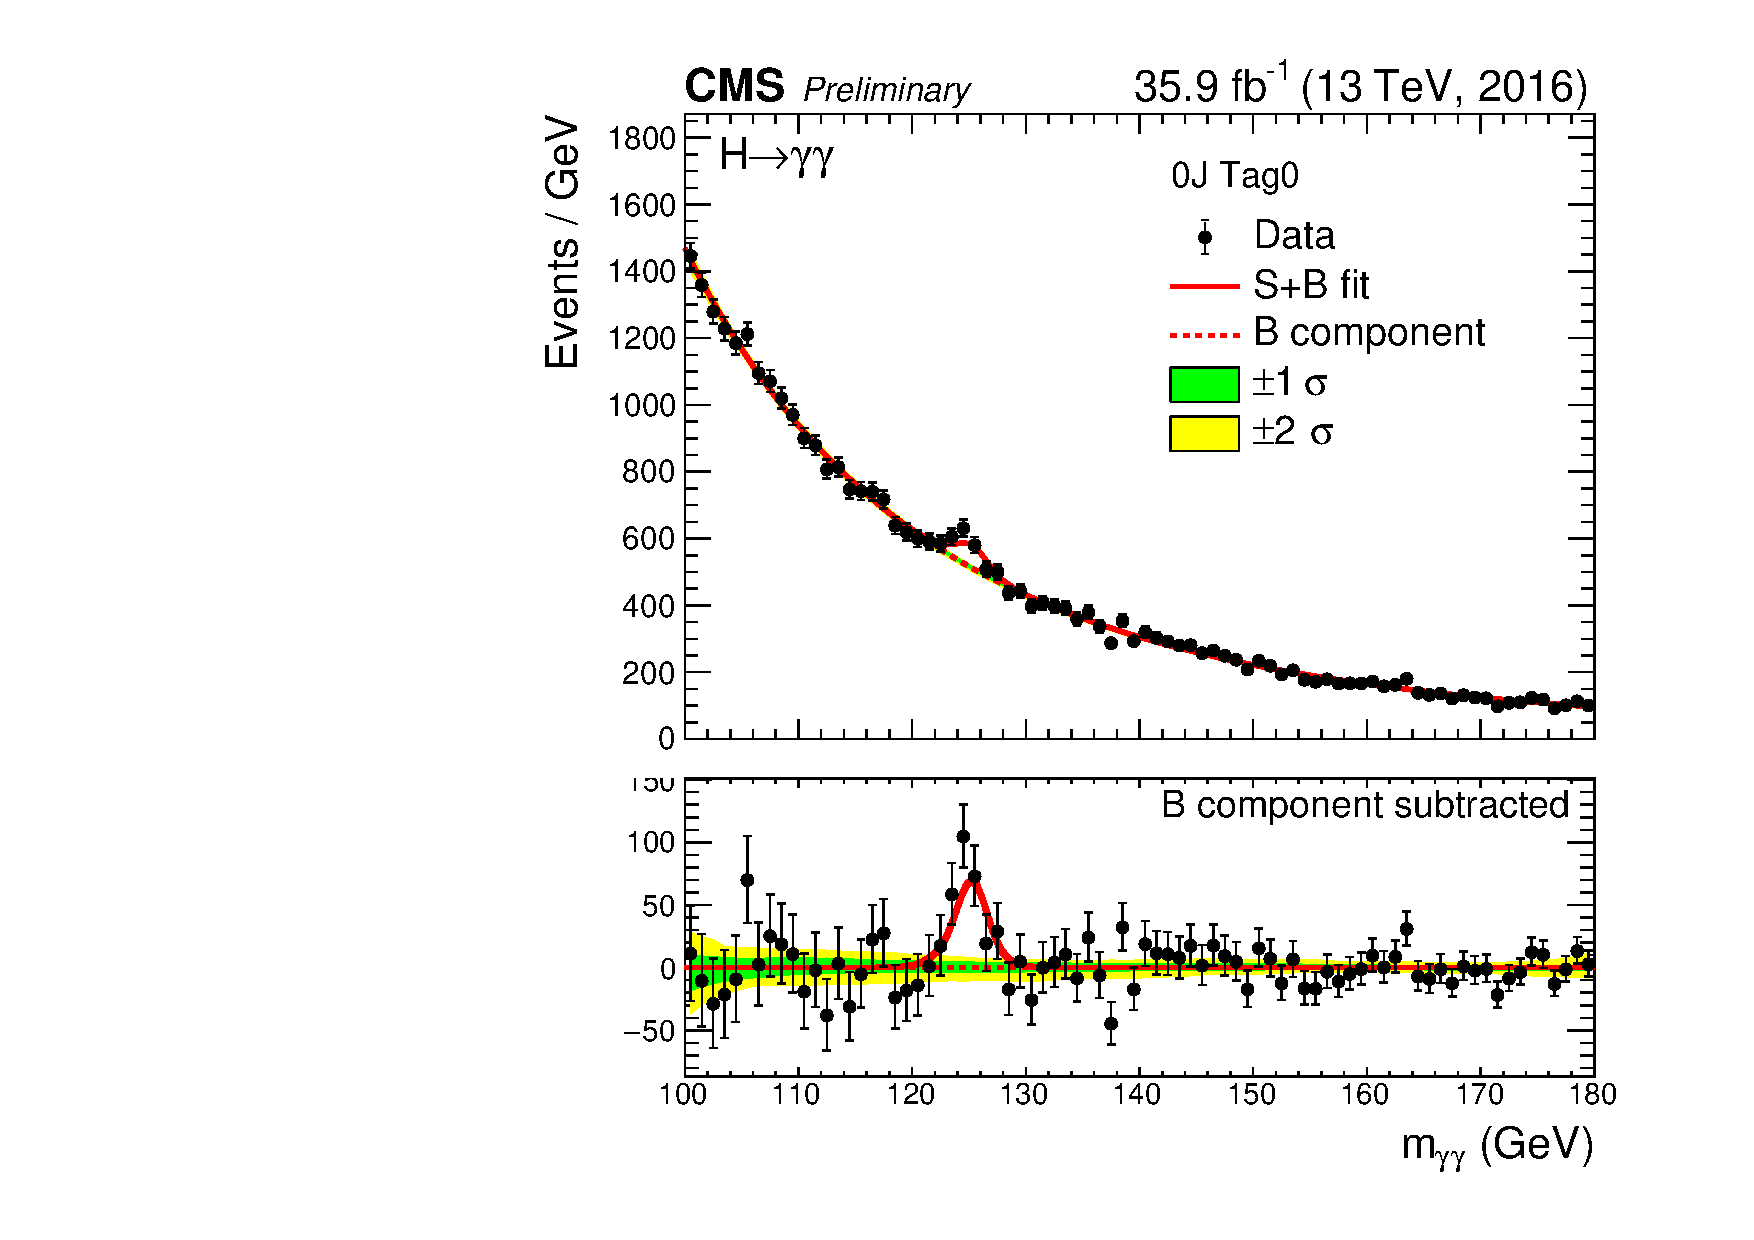
\includegraphics[width=0.49\textwidth]{Figures/Appendices/_forAppendix2016ch1_RECO_0J_Tag0_13TeV.pdf}
  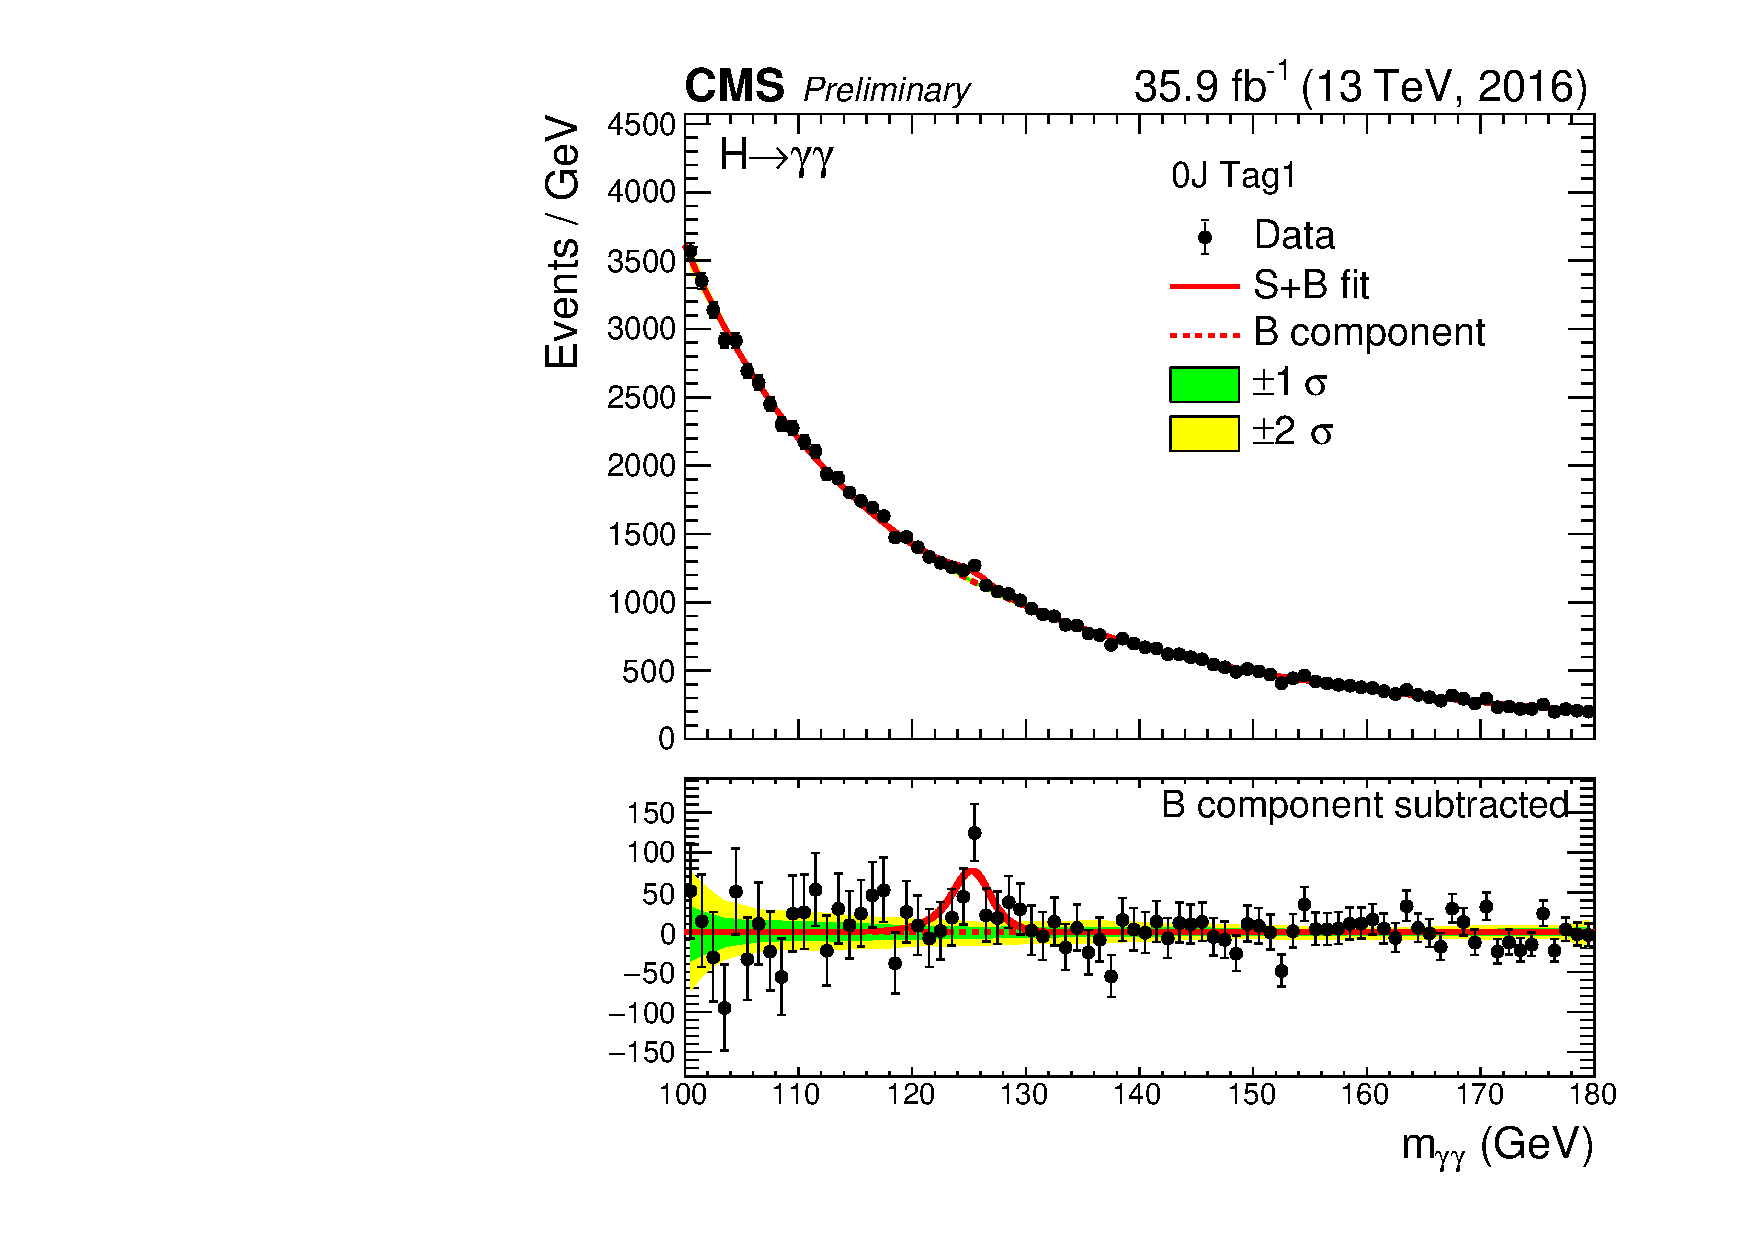
\includegraphics[width=0.49\textwidth]{Figures/Appendices/_forAppendix2016ch1_RECO_0J_Tag1_13TeV.pdf}
  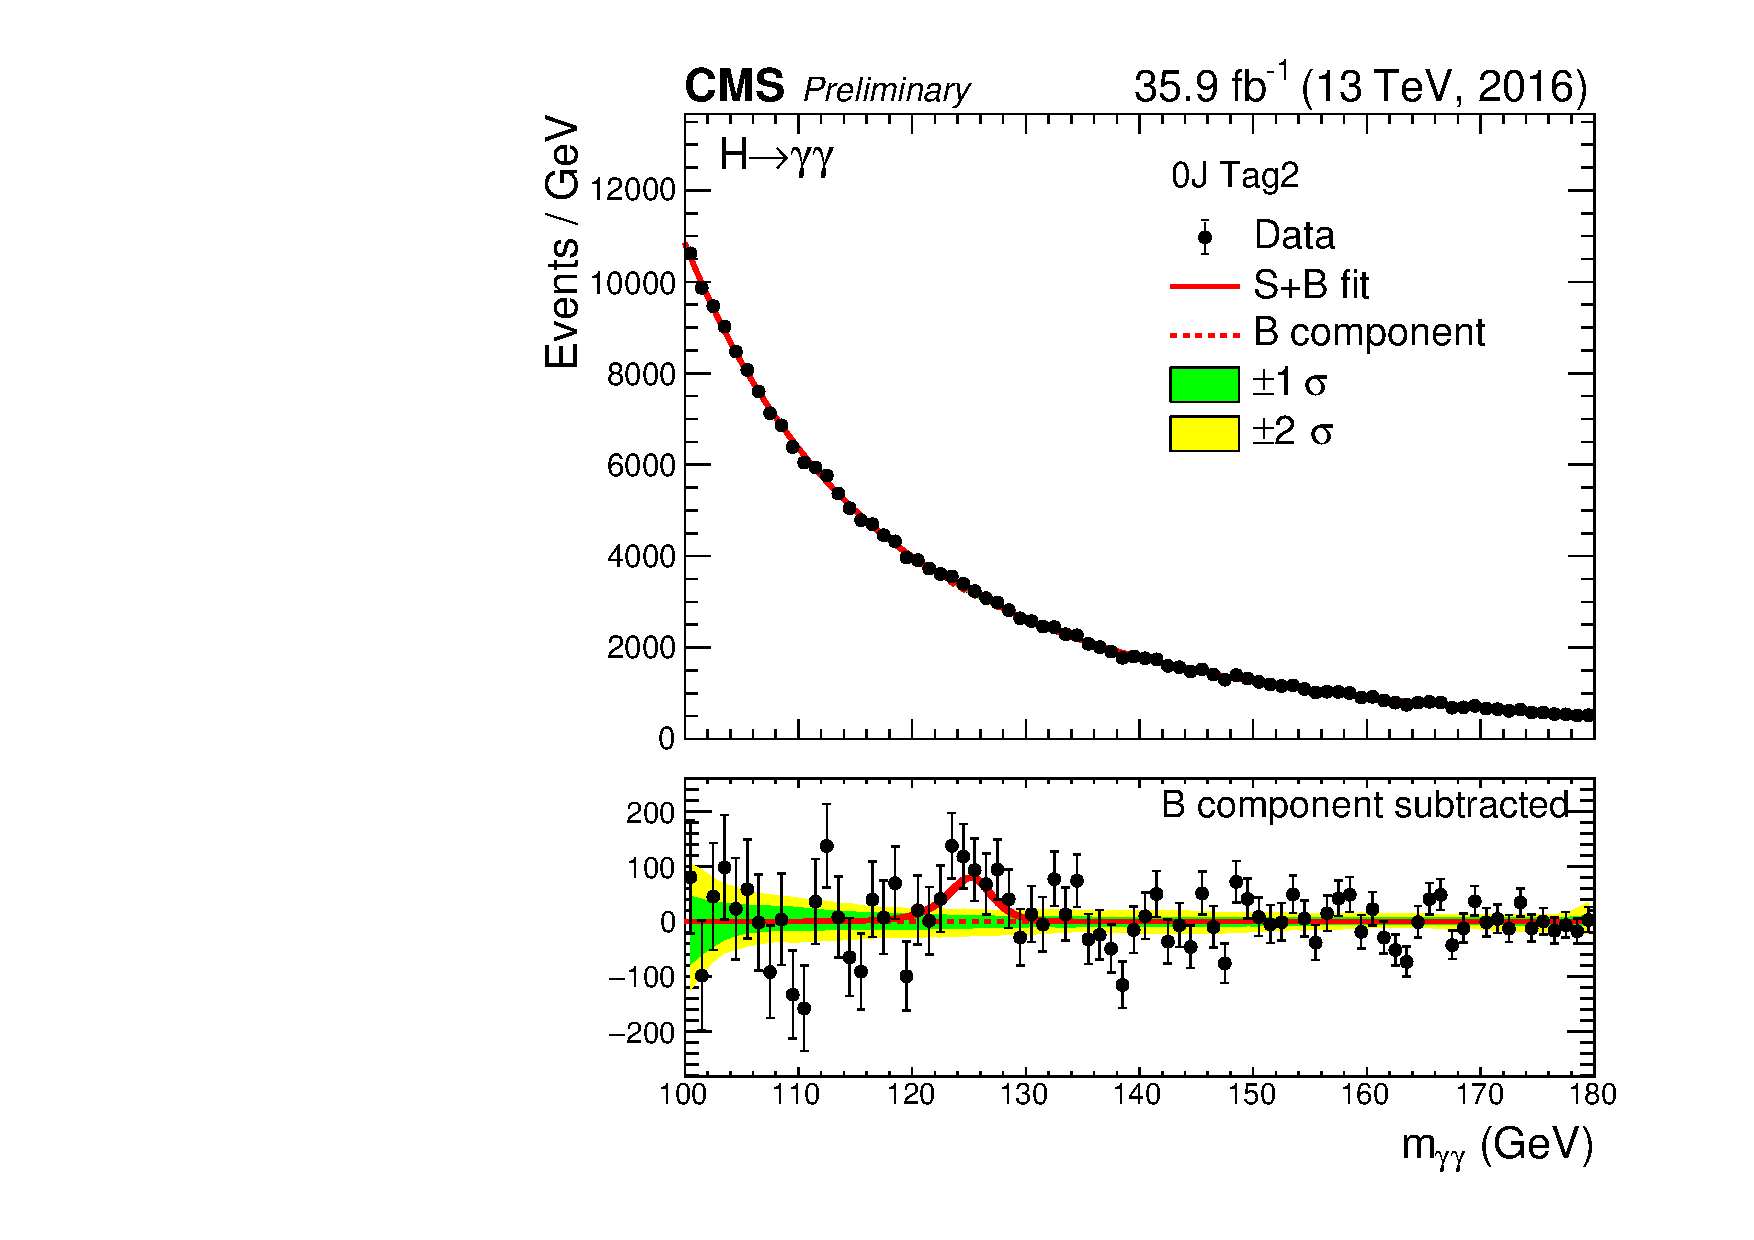
\includegraphics[width=0.49\textwidth]{Figures/Appendices/_forAppendix2016ch1_RECO_0J_Tag2_13TeV.pdf}
  \caption[Signal plus background fits to data.]
  {
    Data points (black) and signal plus background model fit are shown. 
    The one standard deviation (green) and two standard deviation (yellow) bands 
    include the uncertainties in the background component of the fit. 
    The solid red line shows the contribution from the total signal, plus the background contribution. 
    The dashed red line shows the contribution from the background component of the fit. 
    The bottom plot shows the residuals after subtraction of this background component.
  }
\end{figure}

\begin{figure}[hptb]
  \centering
  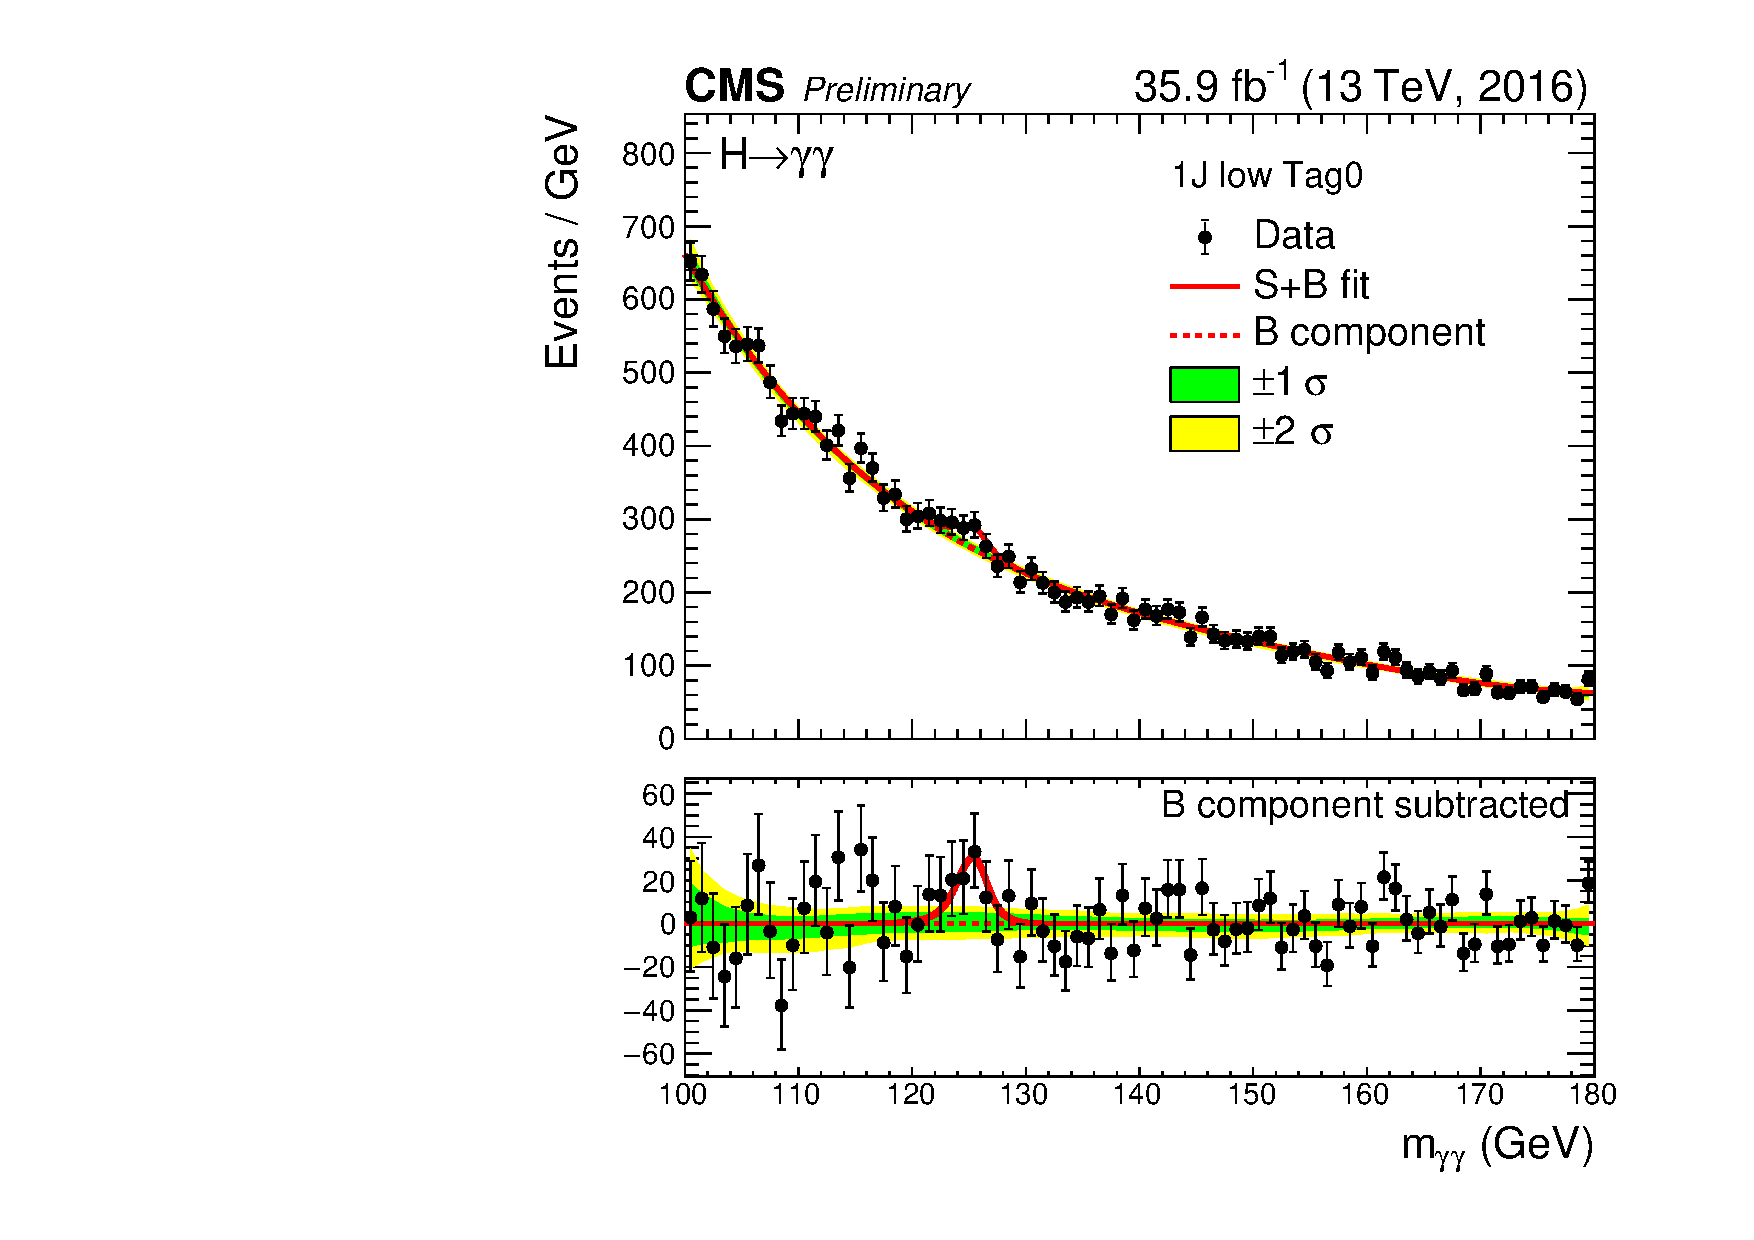
\includegraphics[width=0.49\textwidth]{Figures/Appendices/_forAppendix2016ch1_RECO_1J_PTH_0_60_Tag0_13TeV.pdf}
  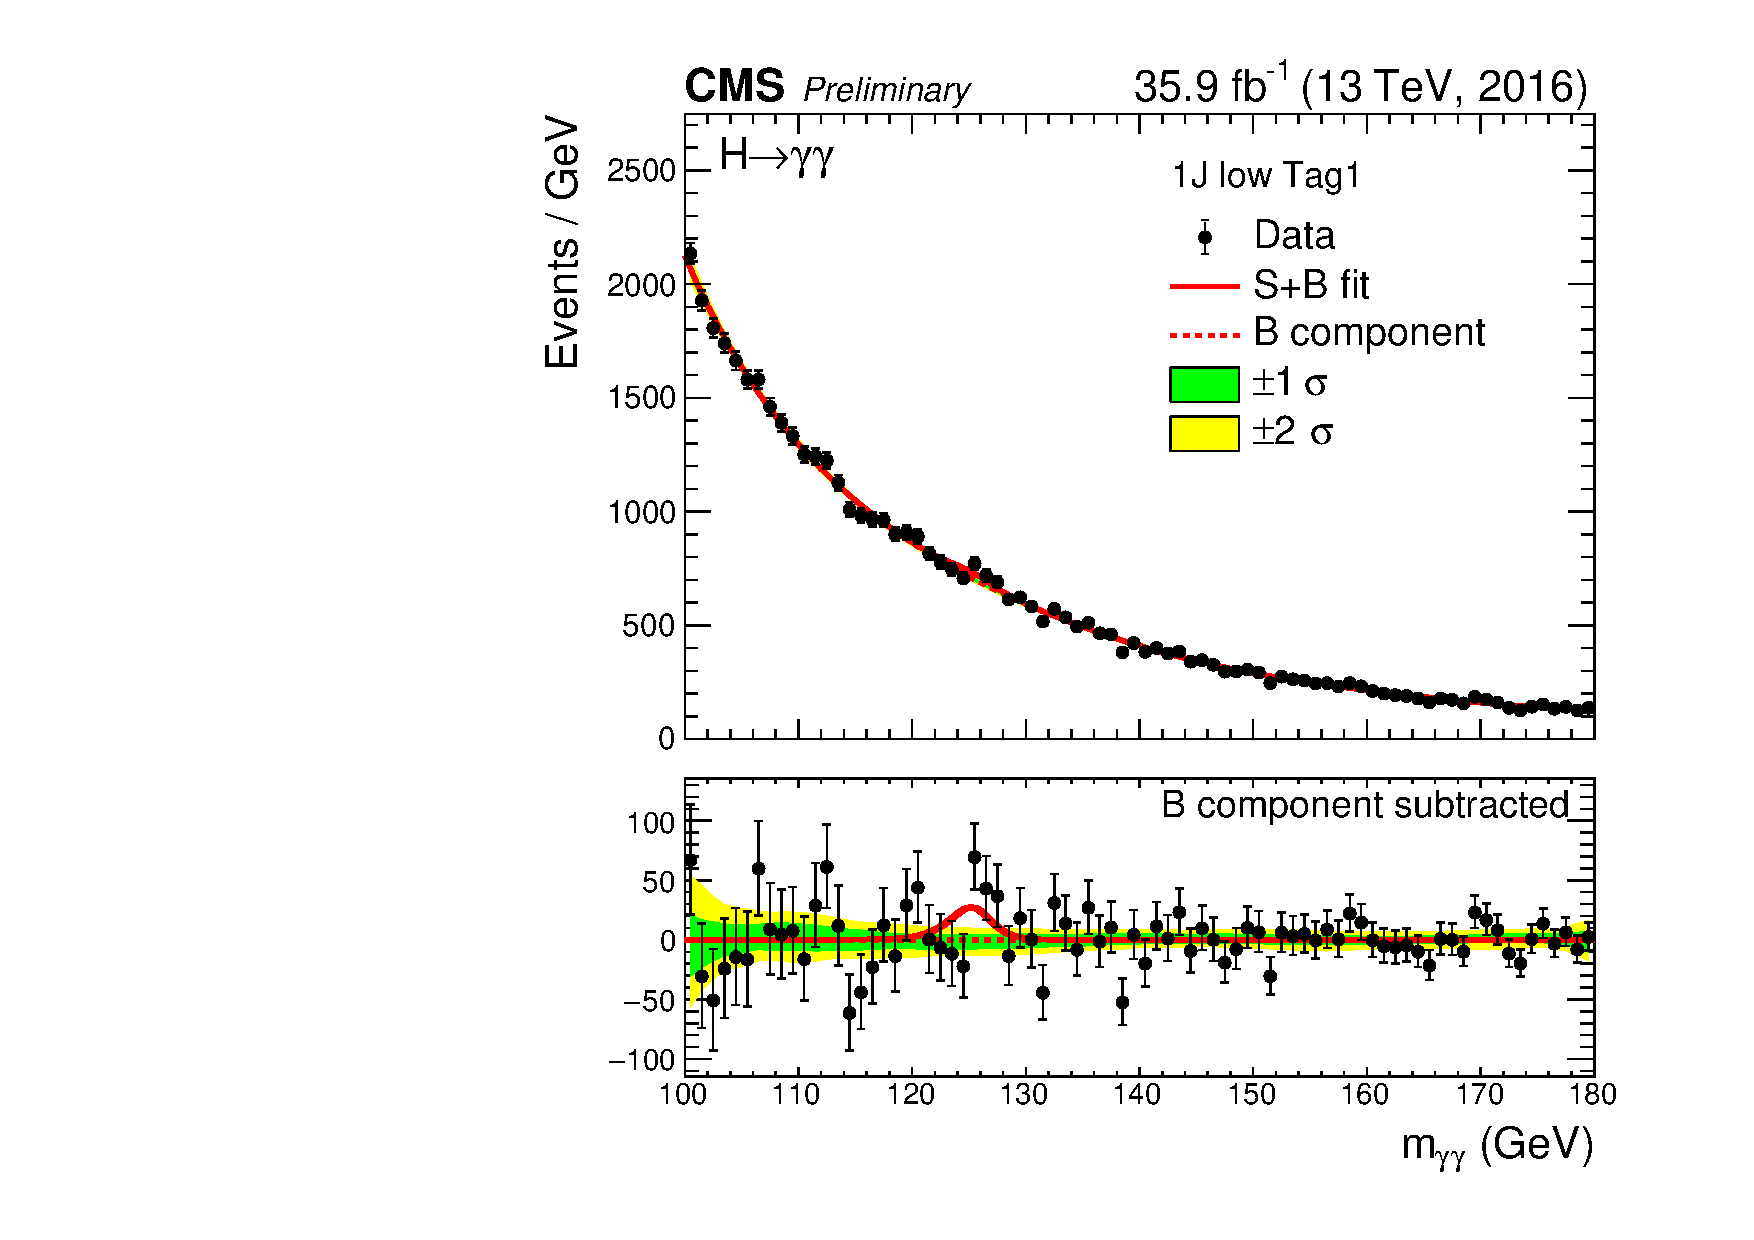
\includegraphics[width=0.49\textwidth]{Figures/Appendices/_forAppendix2016ch1_RECO_1J_PTH_0_60_Tag1_13TeV.pdf}
  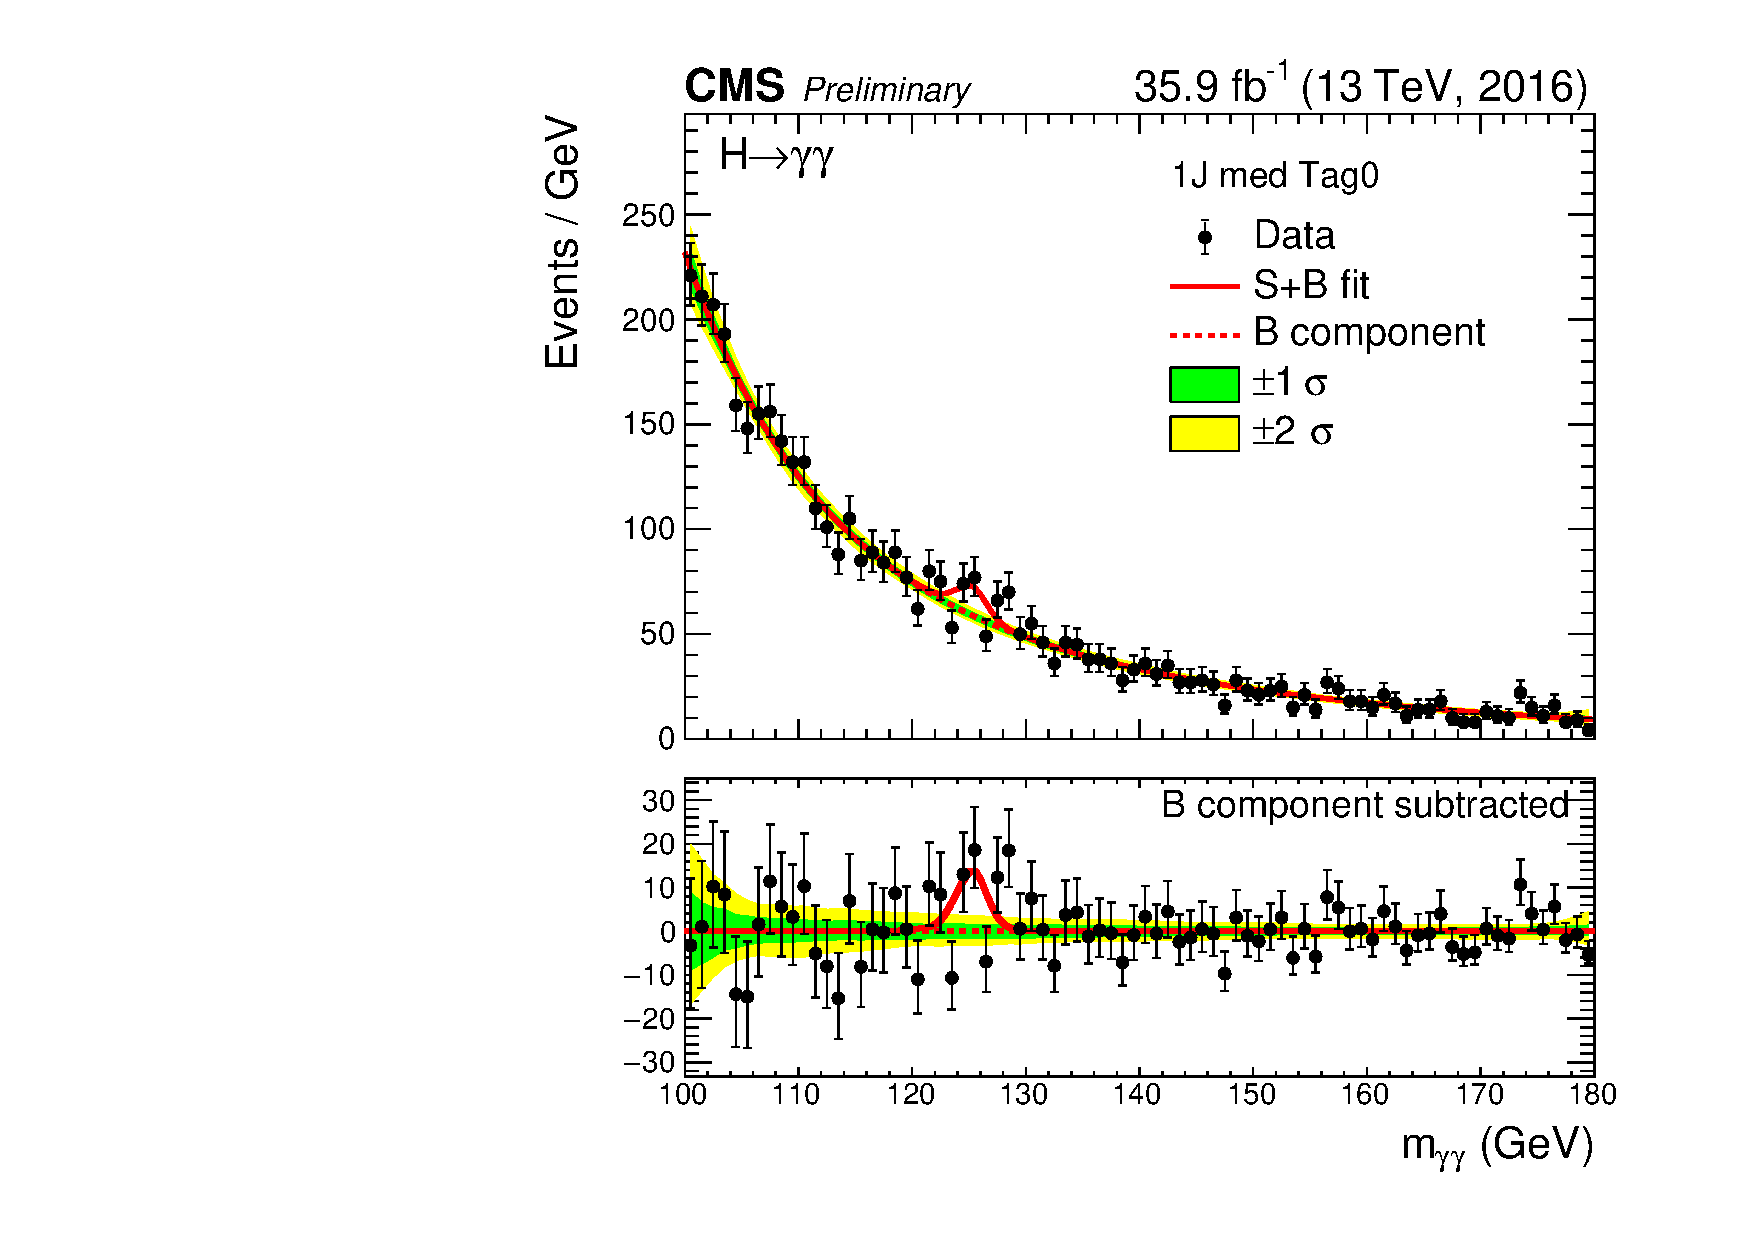
\includegraphics[width=0.49\textwidth]{Figures/Appendices/_forAppendix2016ch1_RECO_1J_PTH_60_120_Tag0_13TeV.pdf}
  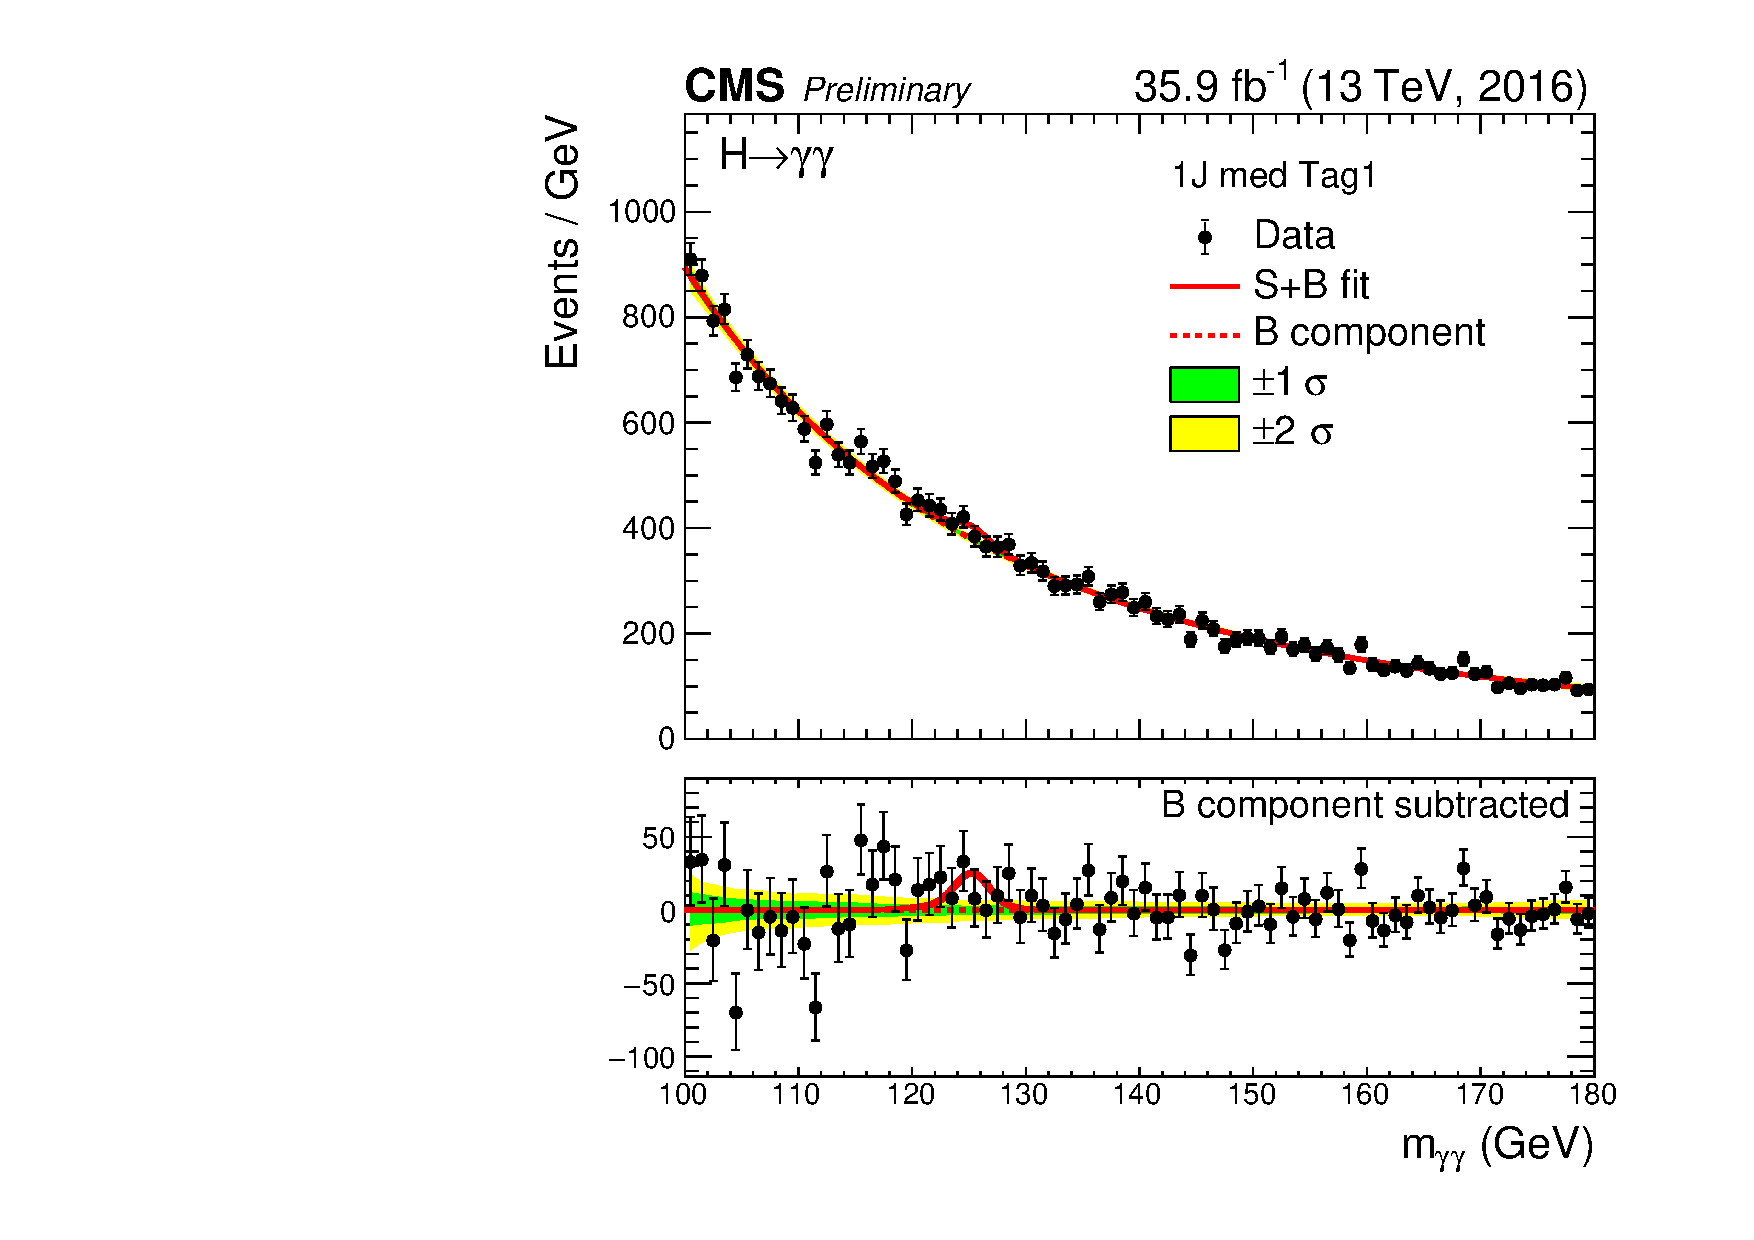
\includegraphics[width=0.49\textwidth]{Figures/Appendices/_forAppendix2016ch1_RECO_1J_PTH_60_120_Tag1_13TeV.pdf}
  \caption[Signal plus background fits to data.]
  {
    Data points (black) and signal plus background model fit are shown. 
    The one standard deviation (green) and two standard deviation (yellow) bands 
    include the uncertainties in the background component of the fit. 
    The solid red line shows the contribution from the total signal, plus the background contribution. 
    The dashed red line shows the contribution from the background component of the fit. 
    The bottom plot shows the residuals after subtraction of this background component.
  }
\end{figure}

\begin{figure}[hptb]
  \centering
  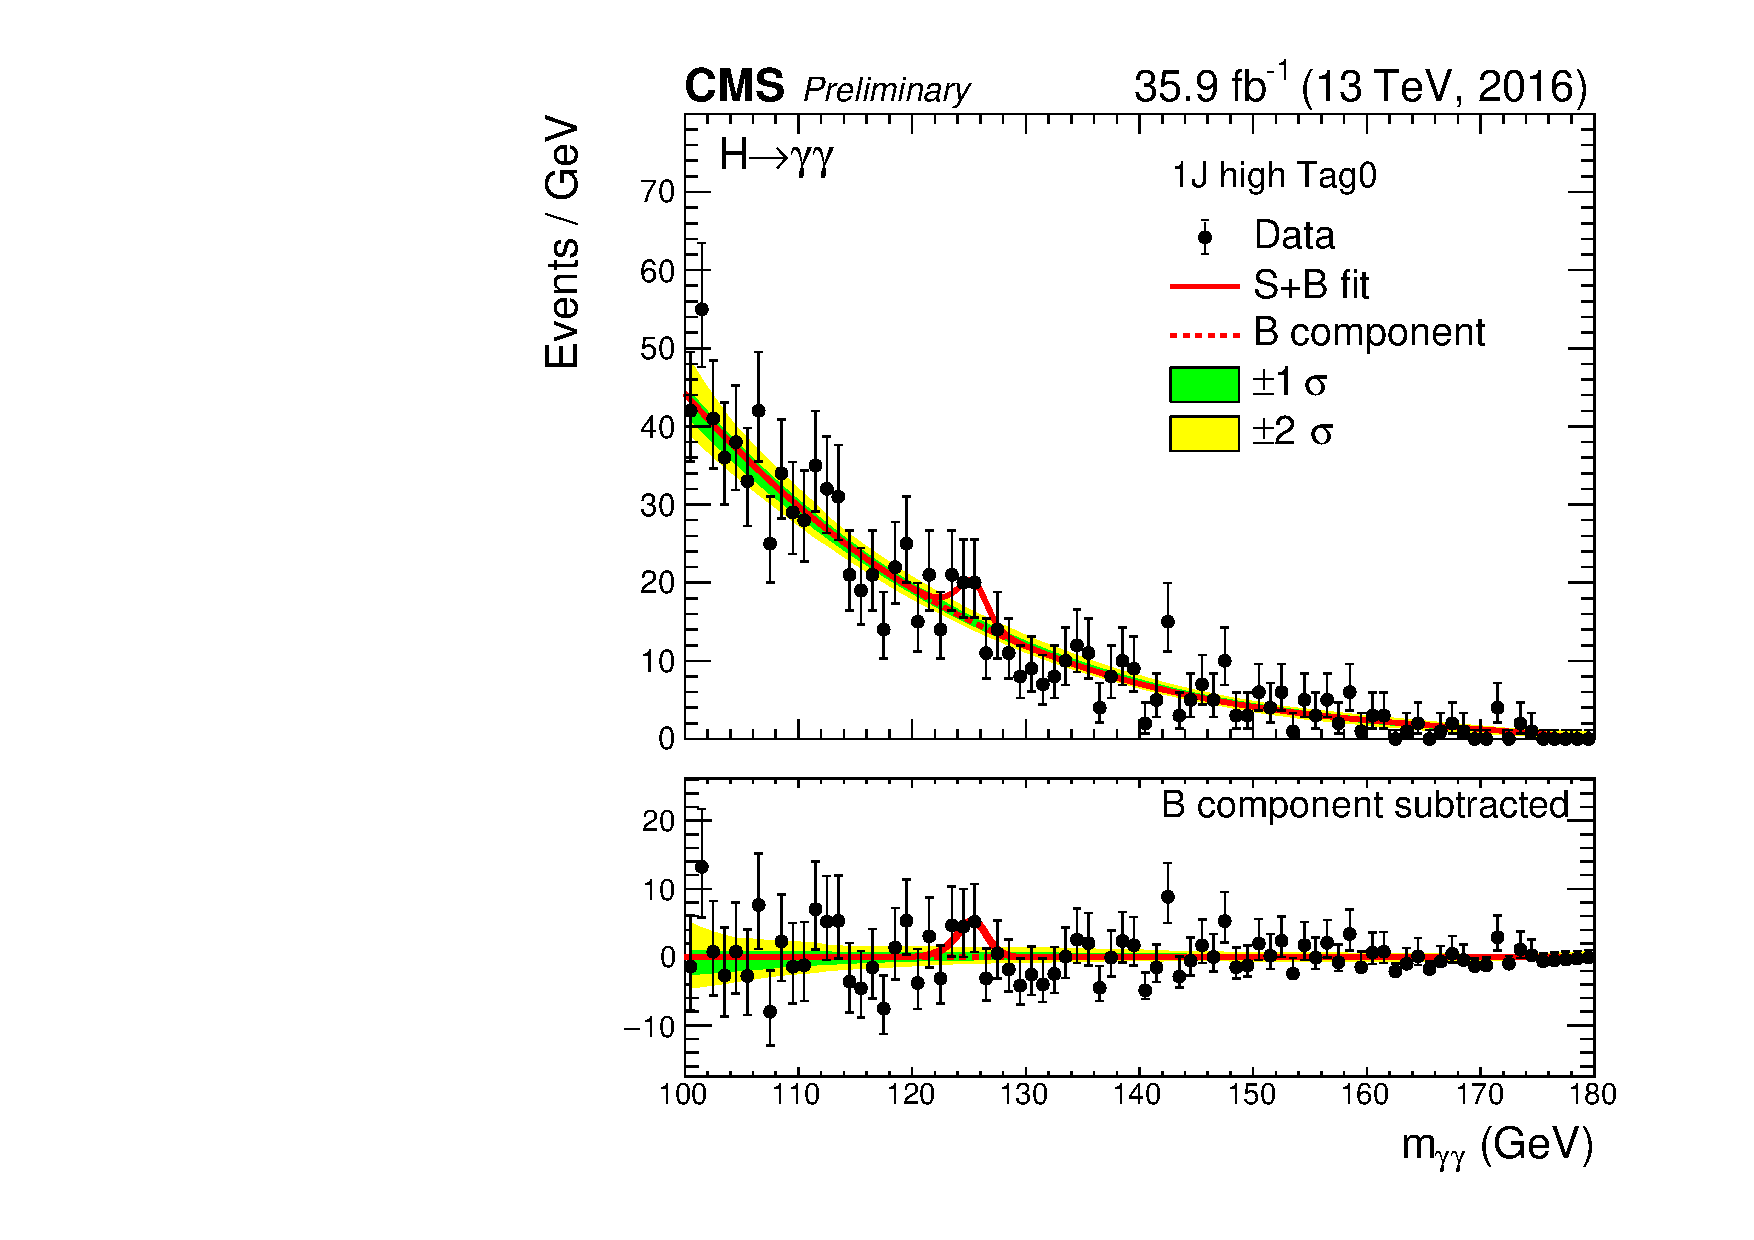
\includegraphics[width=0.49\textwidth]{Figures/Appendices/_forAppendix2016ch1_RECO_1J_PTH_120_200_Tag0_13TeV.pdf}
  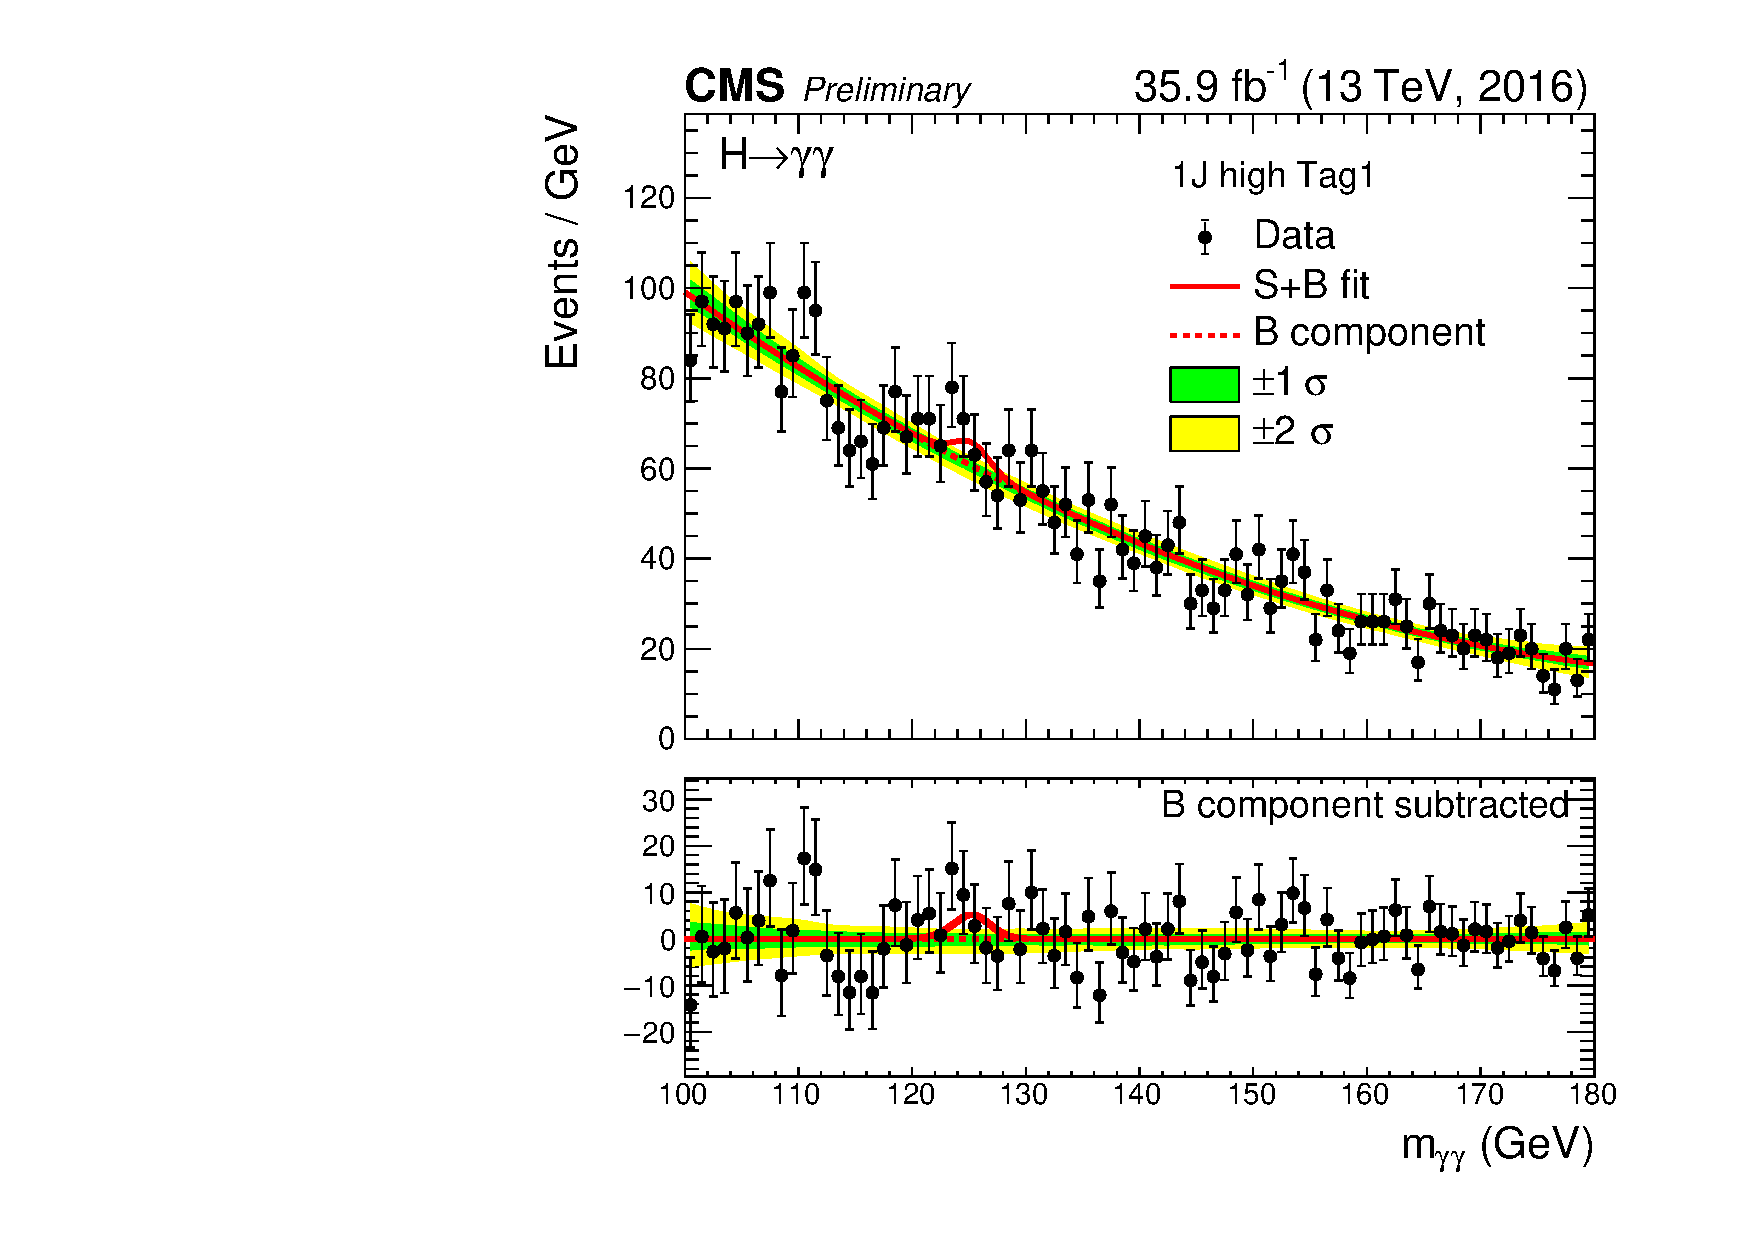
\includegraphics[width=0.49\textwidth]{Figures/Appendices/_forAppendix2016ch1_RECO_1J_PTH_120_200_Tag1_13TeV.pdf}
  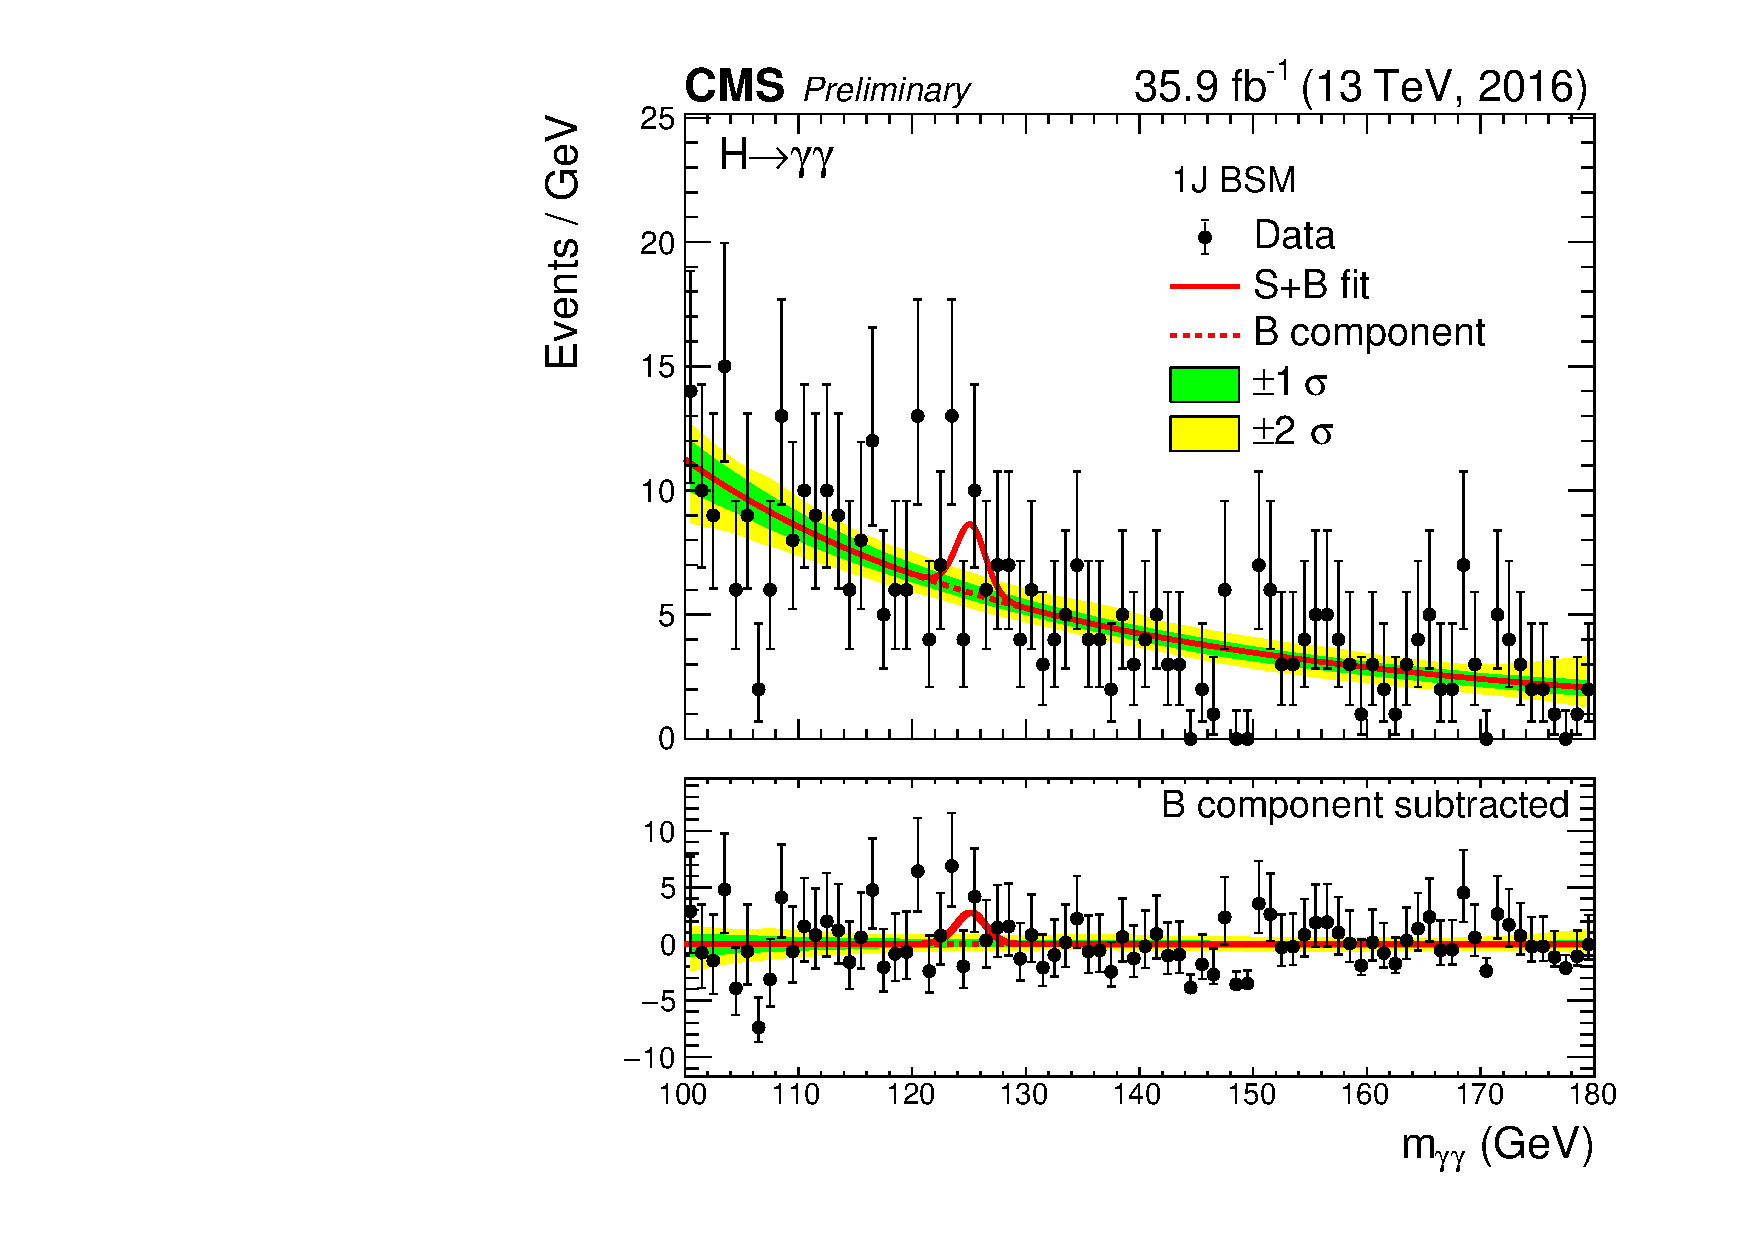
\includegraphics[width=0.49\textwidth]{Figures/Appendices/_forAppendix2016ch1_RECO_1J_PTH_GT200_13TeV.pdf}
  \caption[Signal plus background fits to data.]
  {
    Data points (black) and signal plus background model fit are shown. 
    The one standard deviation (green) and two standard deviation (yellow) bands 
    include the uncertainties in the background component of the fit. 
    The solid red line shows the contribution from the total signal, plus the background contribution. 
    The dashed red line shows the contribution from the background component of the fit. 
    The bottom plot shows the residuals after subtraction of this background component.
  }
\end{figure}

\begin{figure}[hptb]
  \centering
  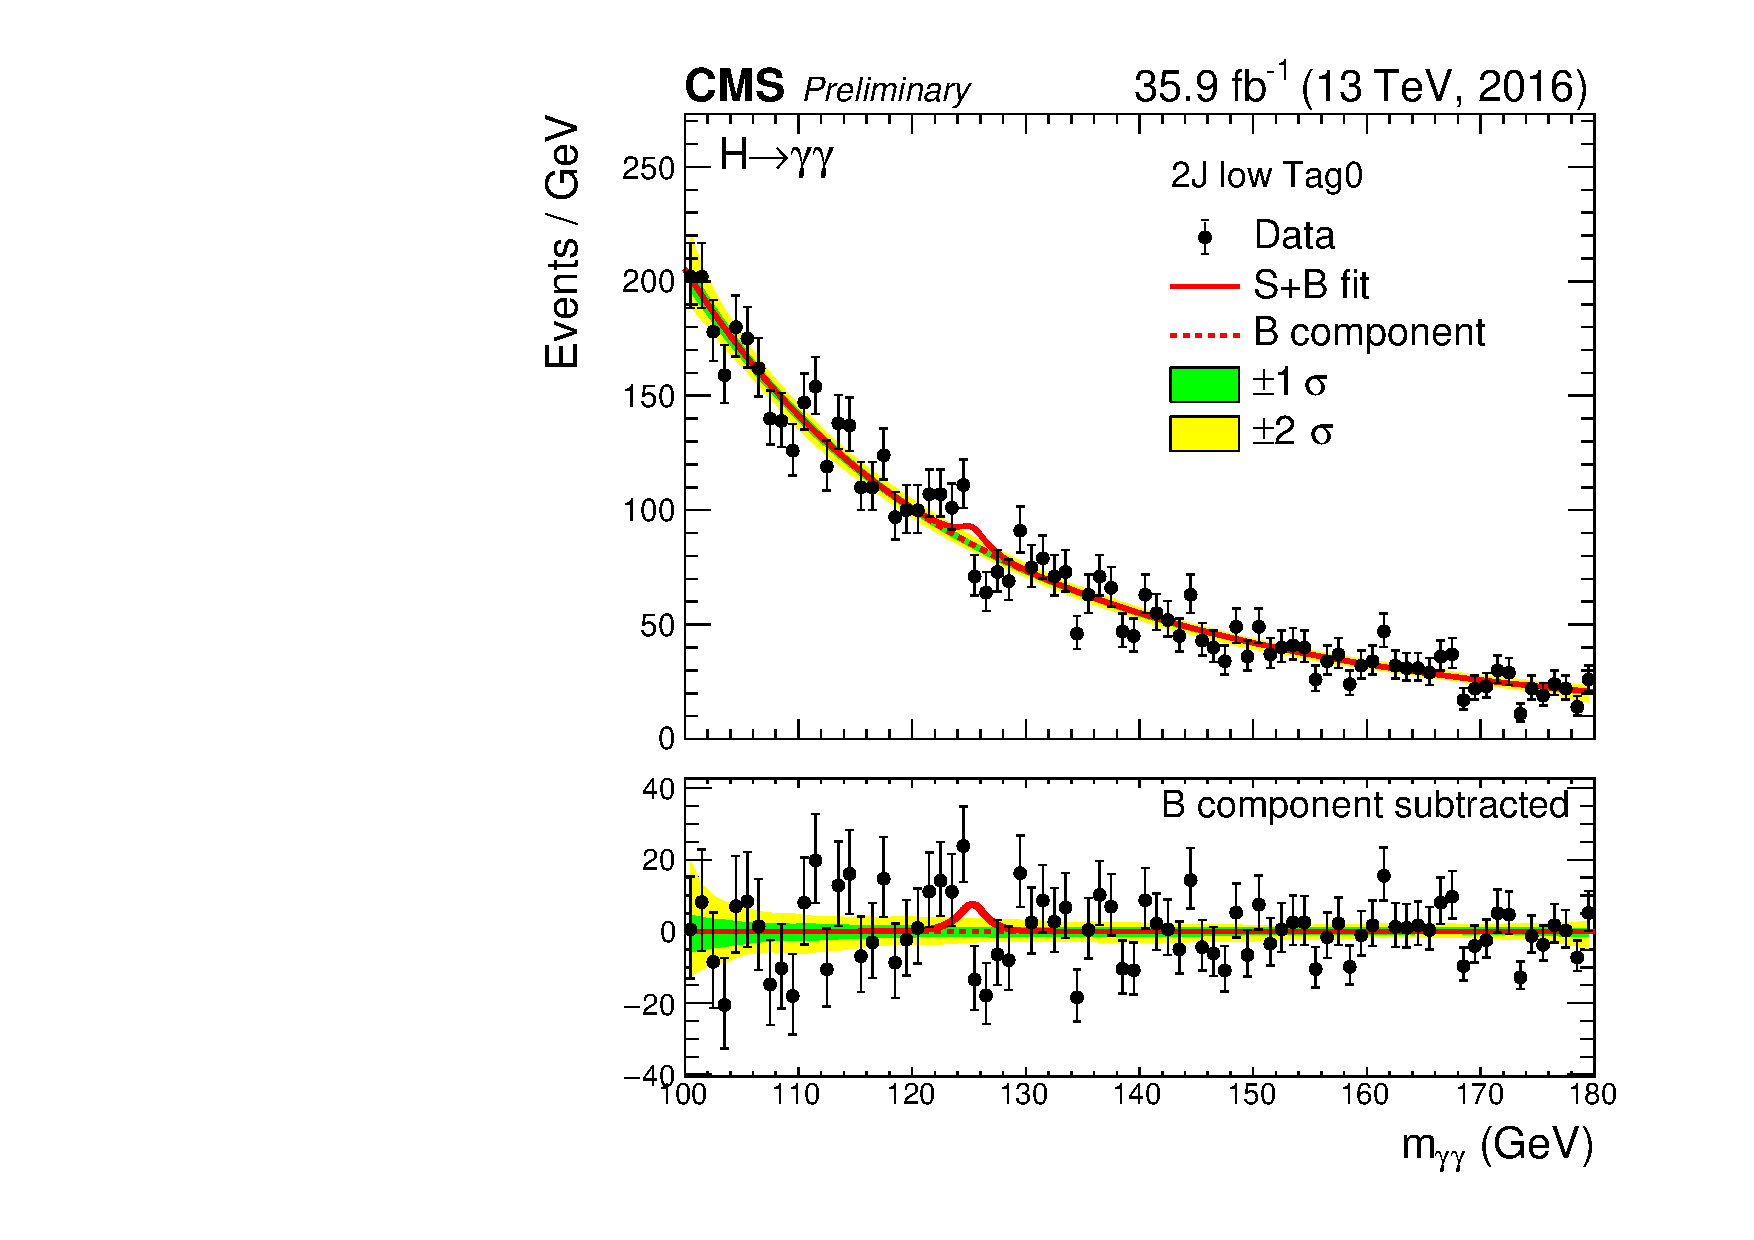
\includegraphics[width=0.49\textwidth]{Figures/Appendices/_forAppendix2016ch1_RECO_GE2J_PTH_0_60_Tag0_13TeV.pdf}
  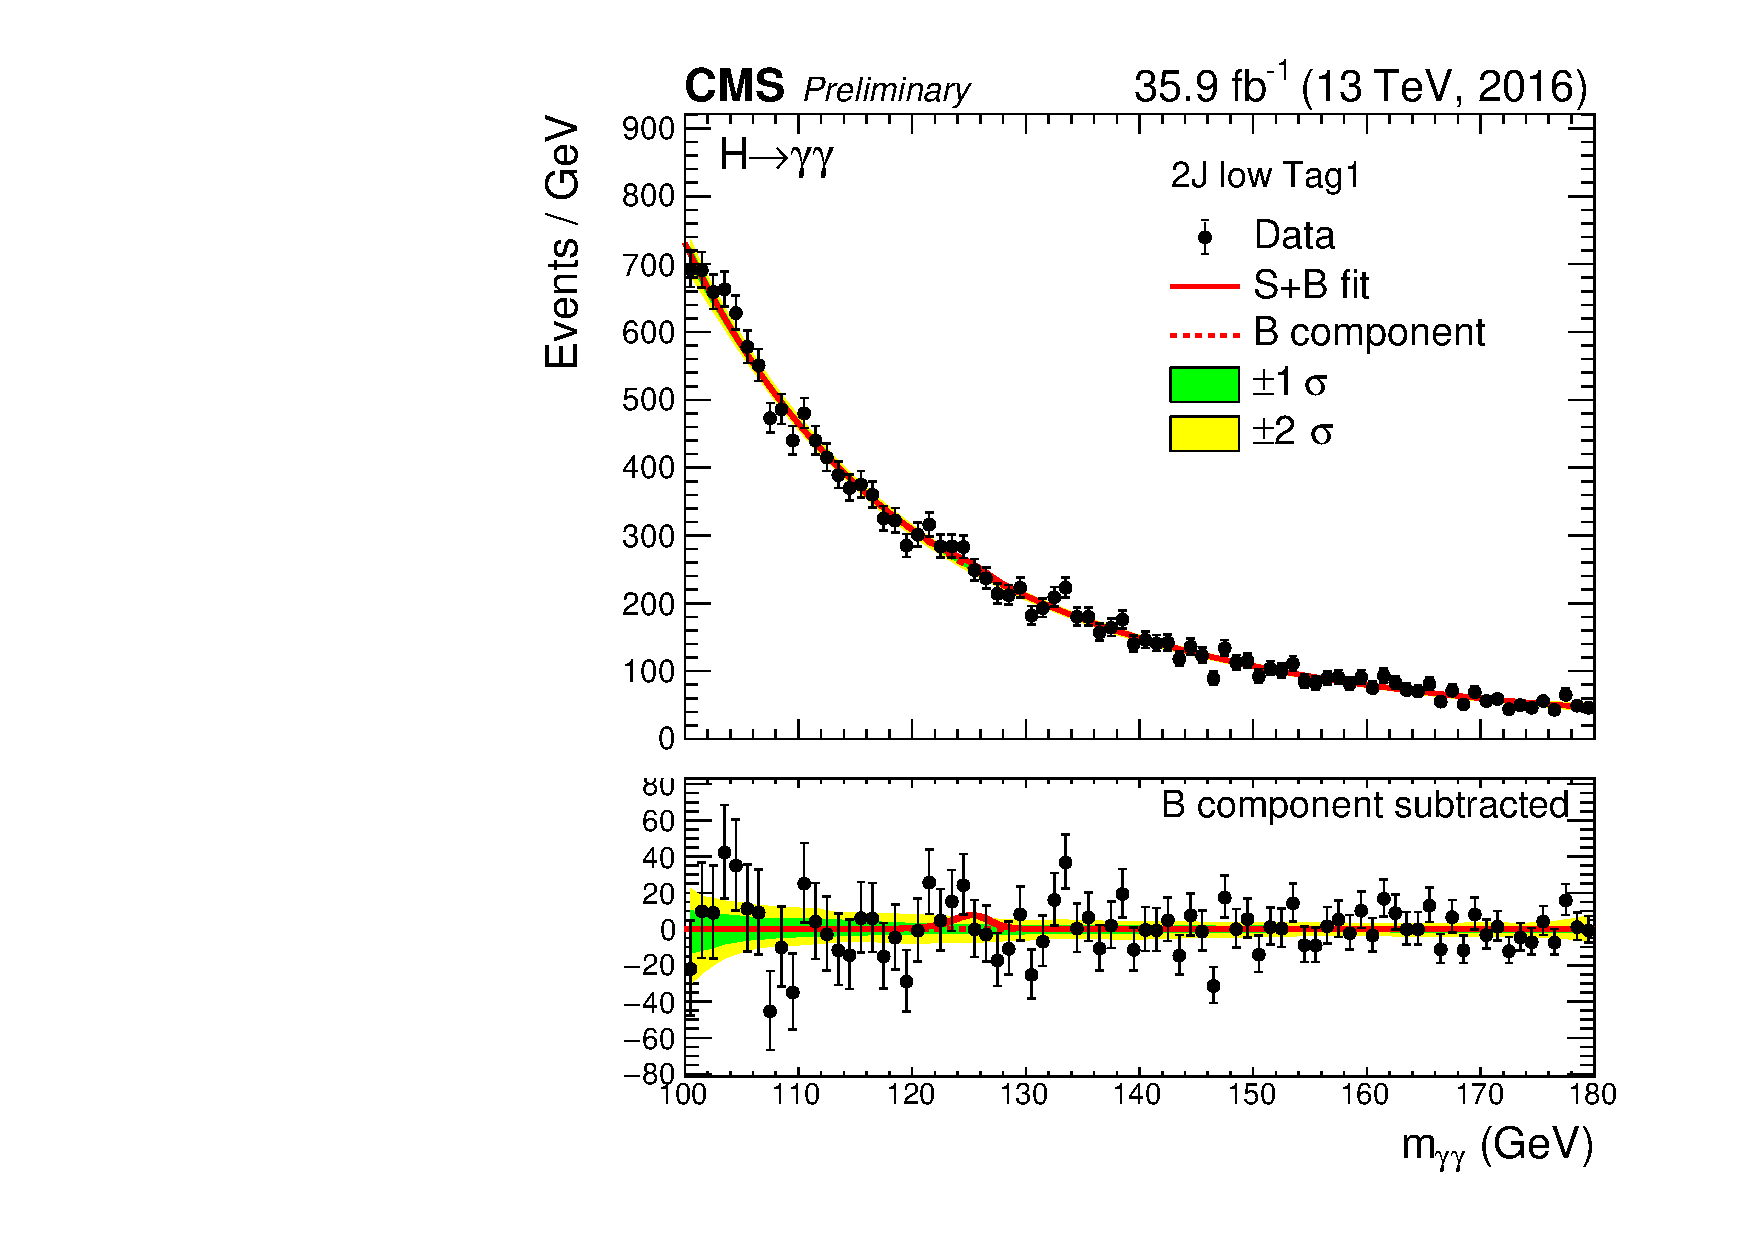
\includegraphics[width=0.49\textwidth]{Figures/Appendices/_forAppendix2016ch1_RECO_GE2J_PTH_0_60_Tag1_13TeV.pdf}
  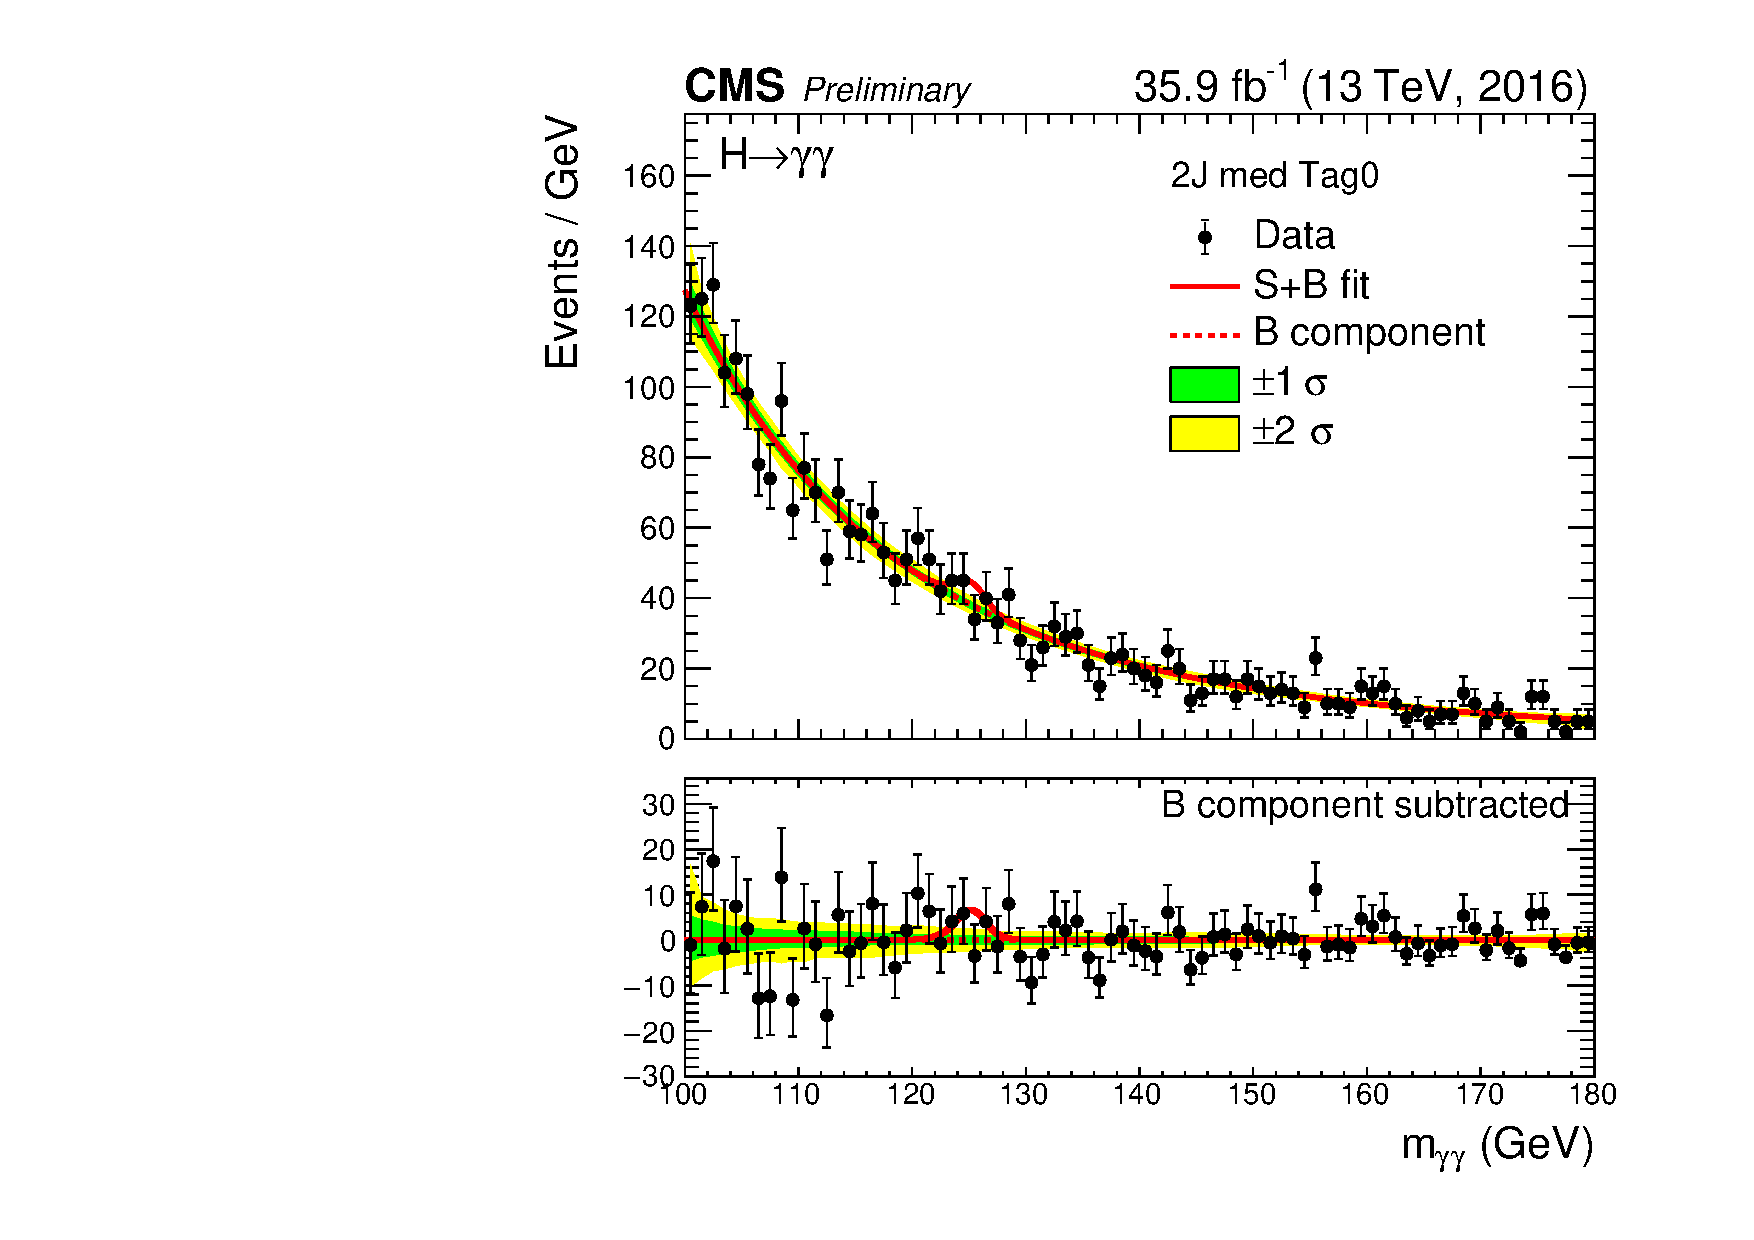
\includegraphics[width=0.49\textwidth]{Figures/Appendices/_forAppendix2016ch1_RECO_GE2J_PTH_60_120_Tag0_13TeV.pdf}
  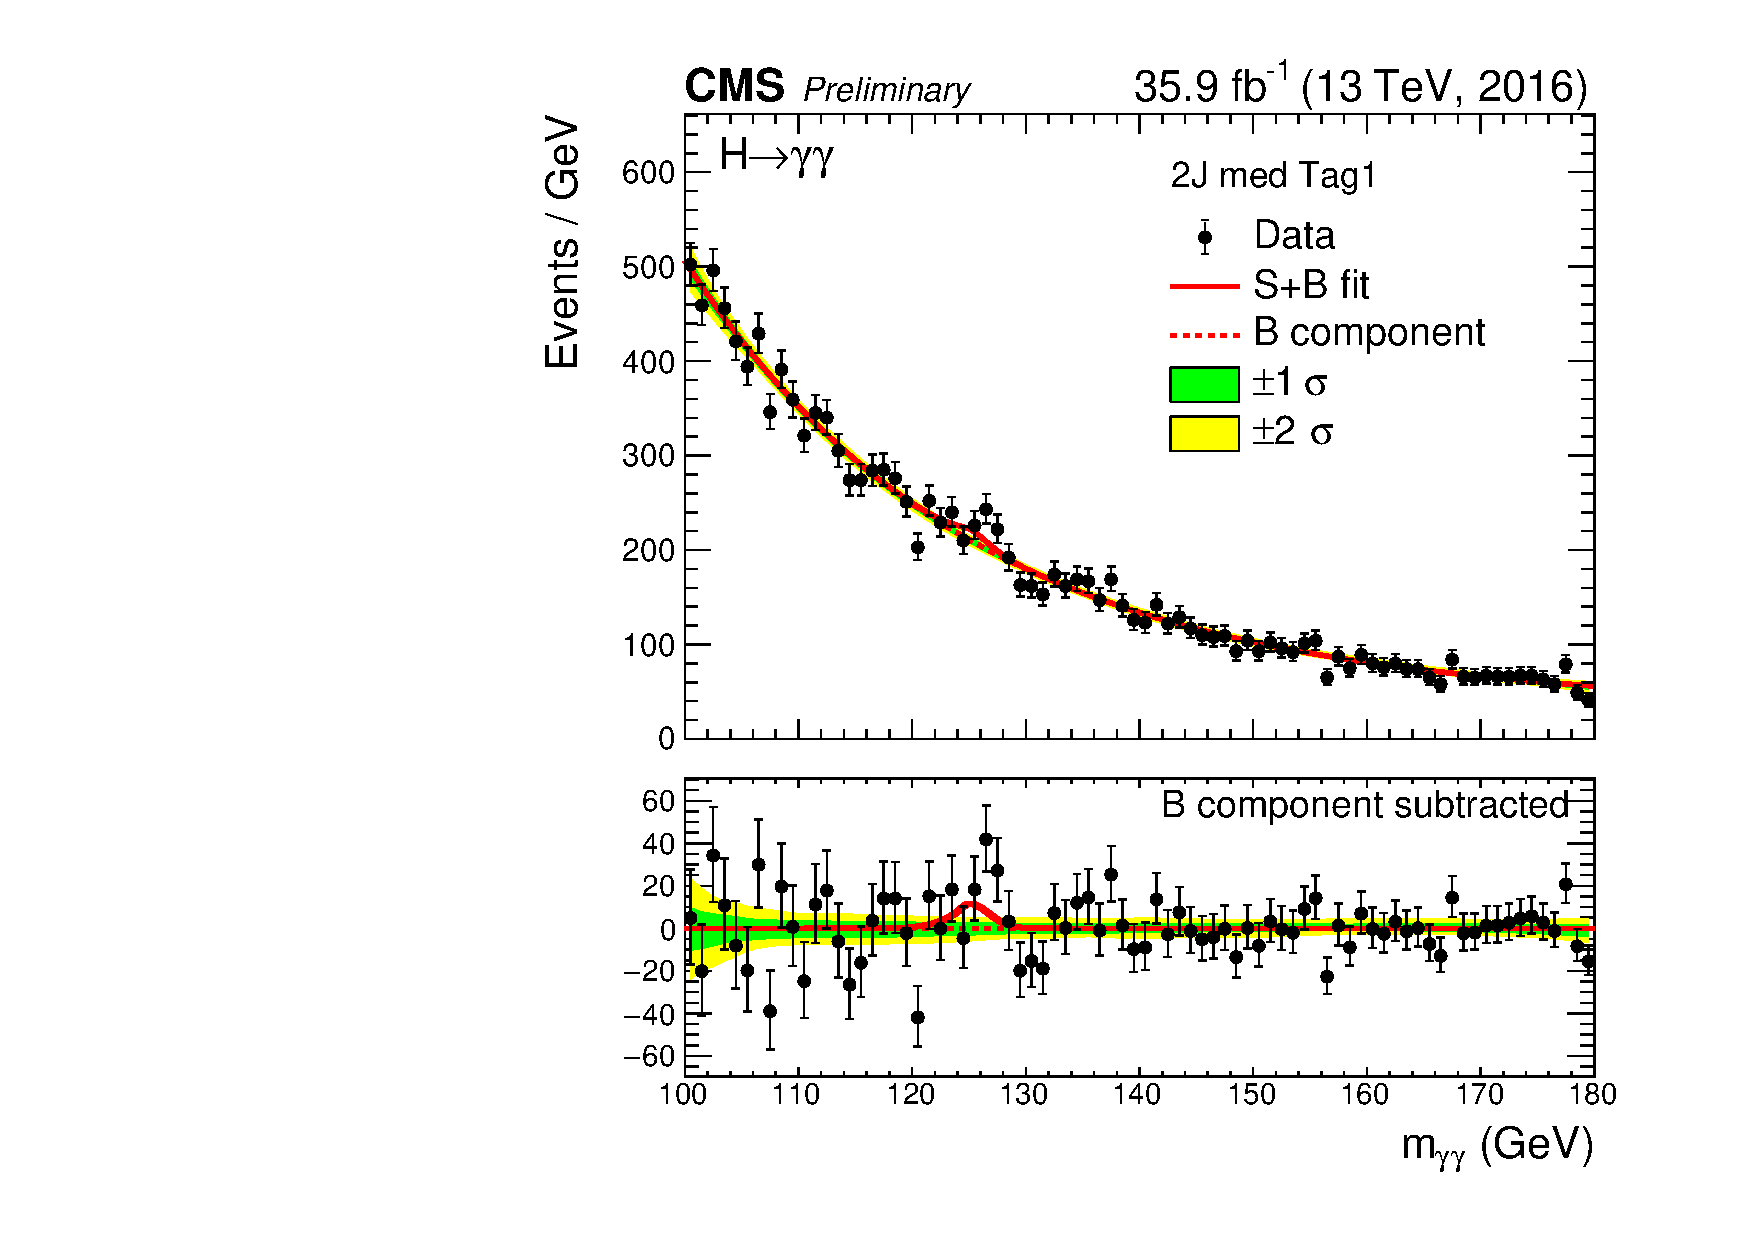
\includegraphics[width=0.49\textwidth]{Figures/Appendices/_forAppendix2016ch1_RECO_GE2J_PTH_60_120_Tag1_13TeV.pdf}
  \caption[Signal plus background fits to data.]
  {
    Data points (black) and signal plus background model fit are shown. 
    The one standard deviation (green) and two standard deviation (yellow) bands 
    include the uncertainties in the background component of the fit. 
    The solid red line shows the contribution from the total signal, plus the background contribution. 
    The dashed red line shows the contribution from the background component of the fit. 
    The bottom plot shows the residuals after subtraction of this background component.
  }
\end{figure}

\begin{figure}[hptb]
  \centering
  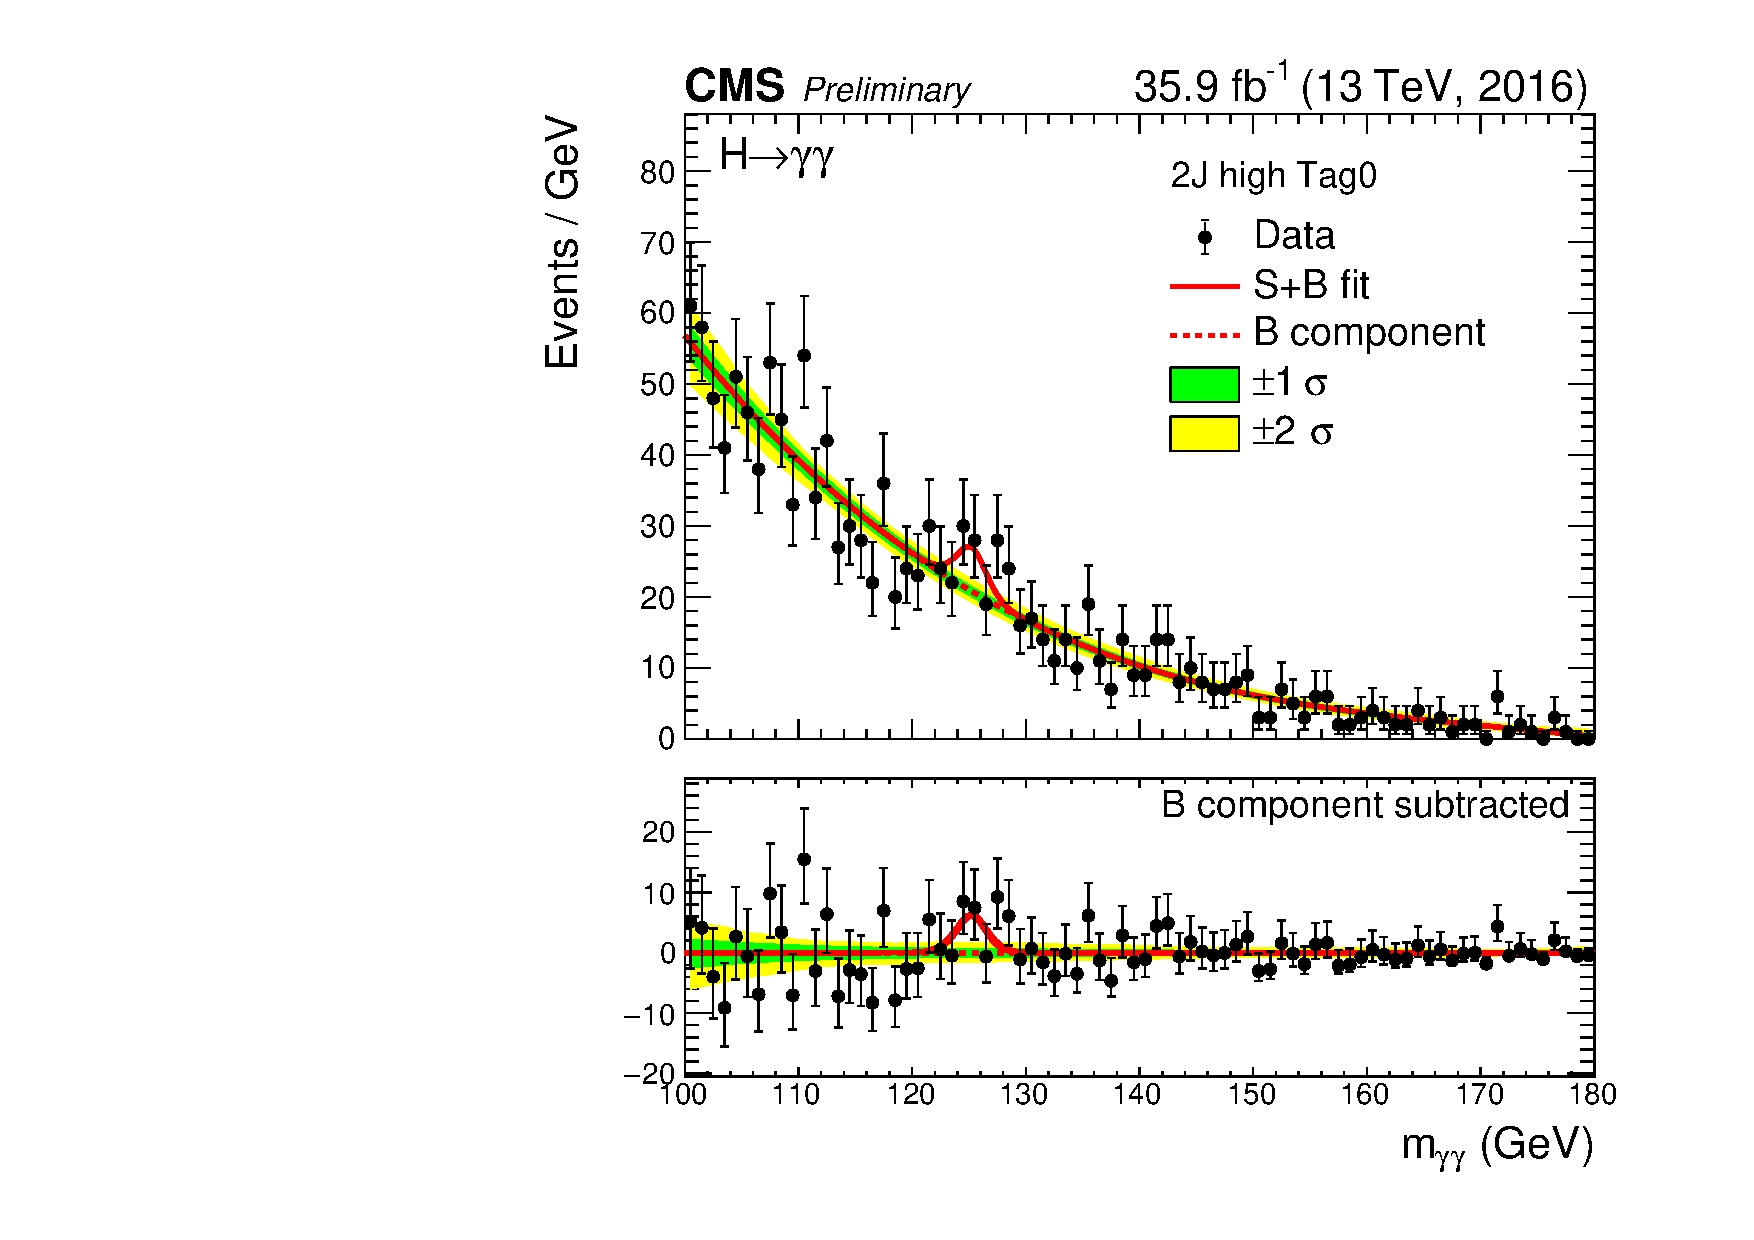
\includegraphics[width=0.49\textwidth]{Figures/Appendices/_forAppendix2016ch1_RECO_GE2J_PTH_120_200_Tag0_13TeV.pdf}
  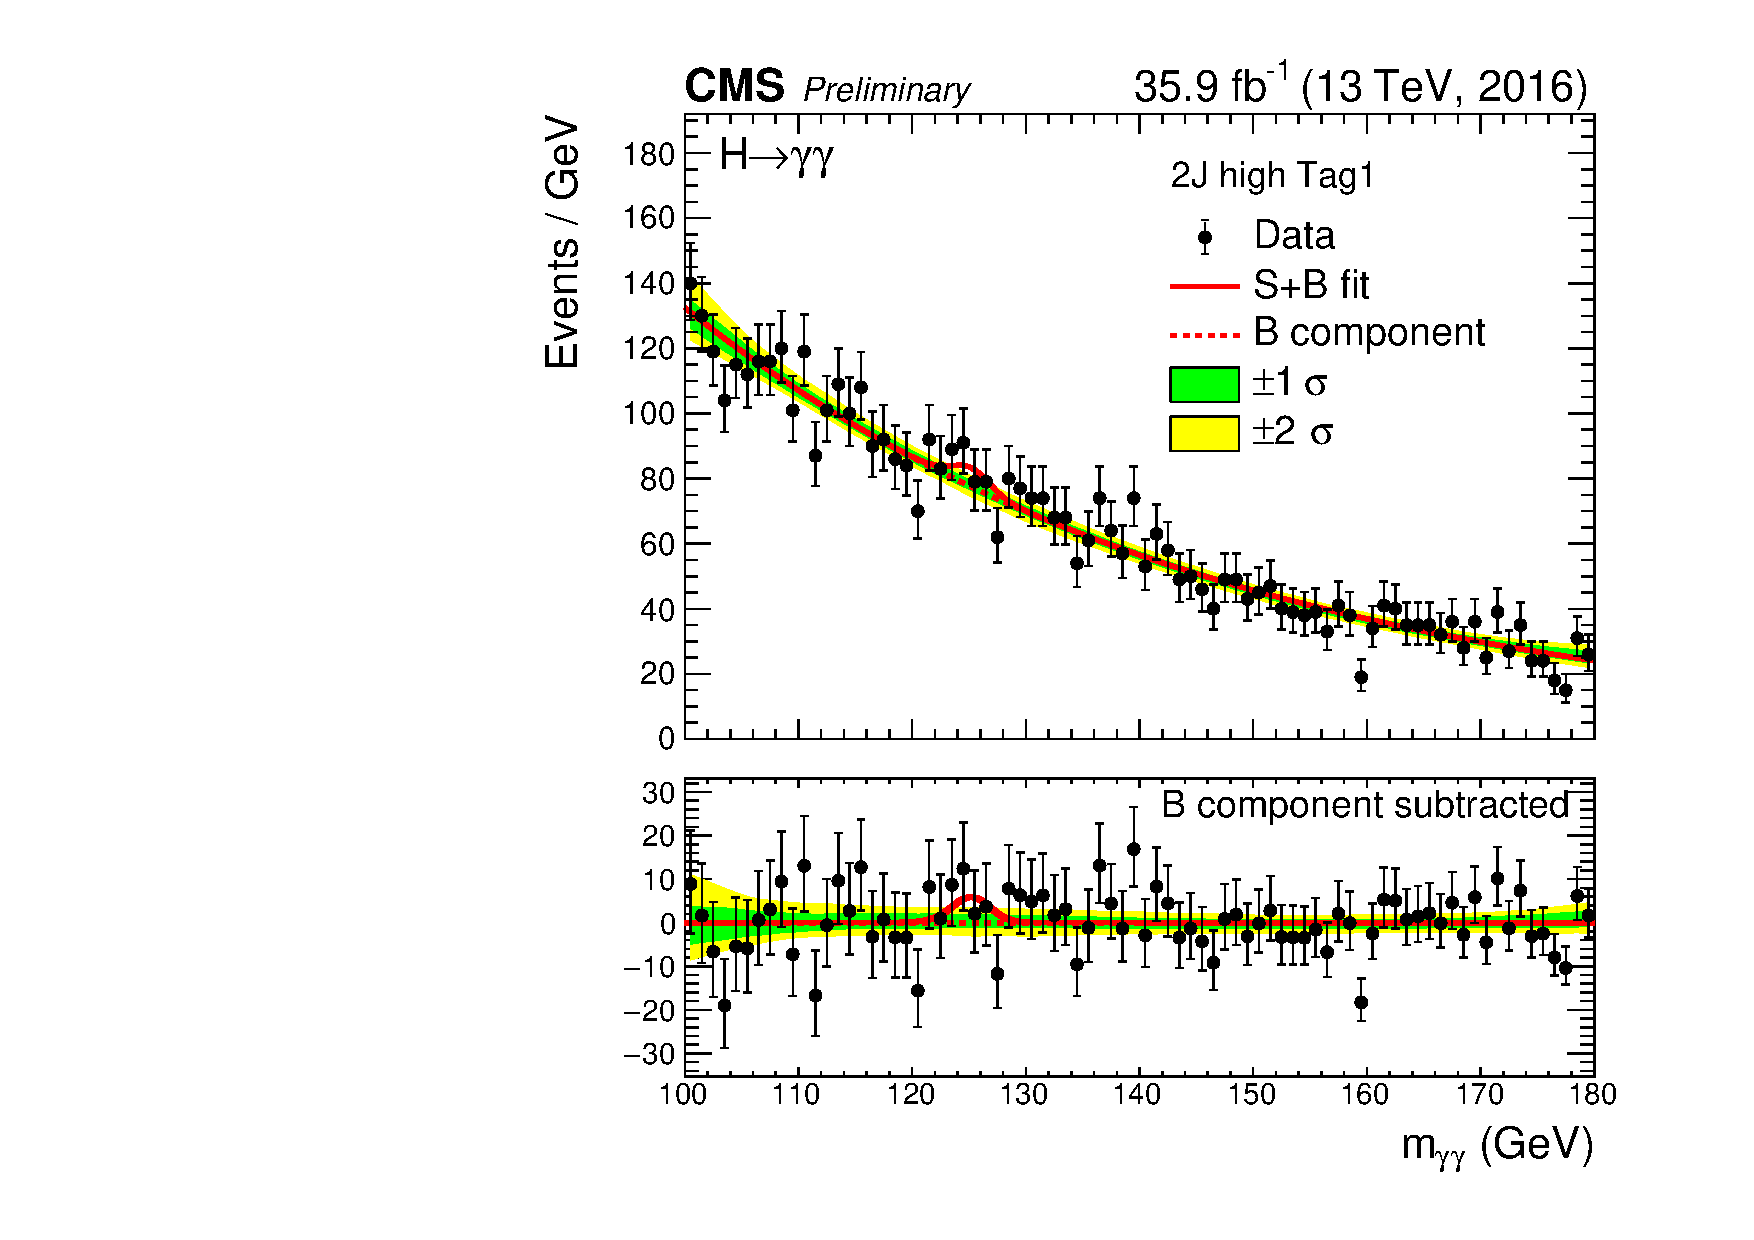
\includegraphics[width=0.49\textwidth]{Figures/Appendices/_forAppendix2016ch1_RECO_GE2J_PTH_120_200_Tag1_13TeV.pdf}
  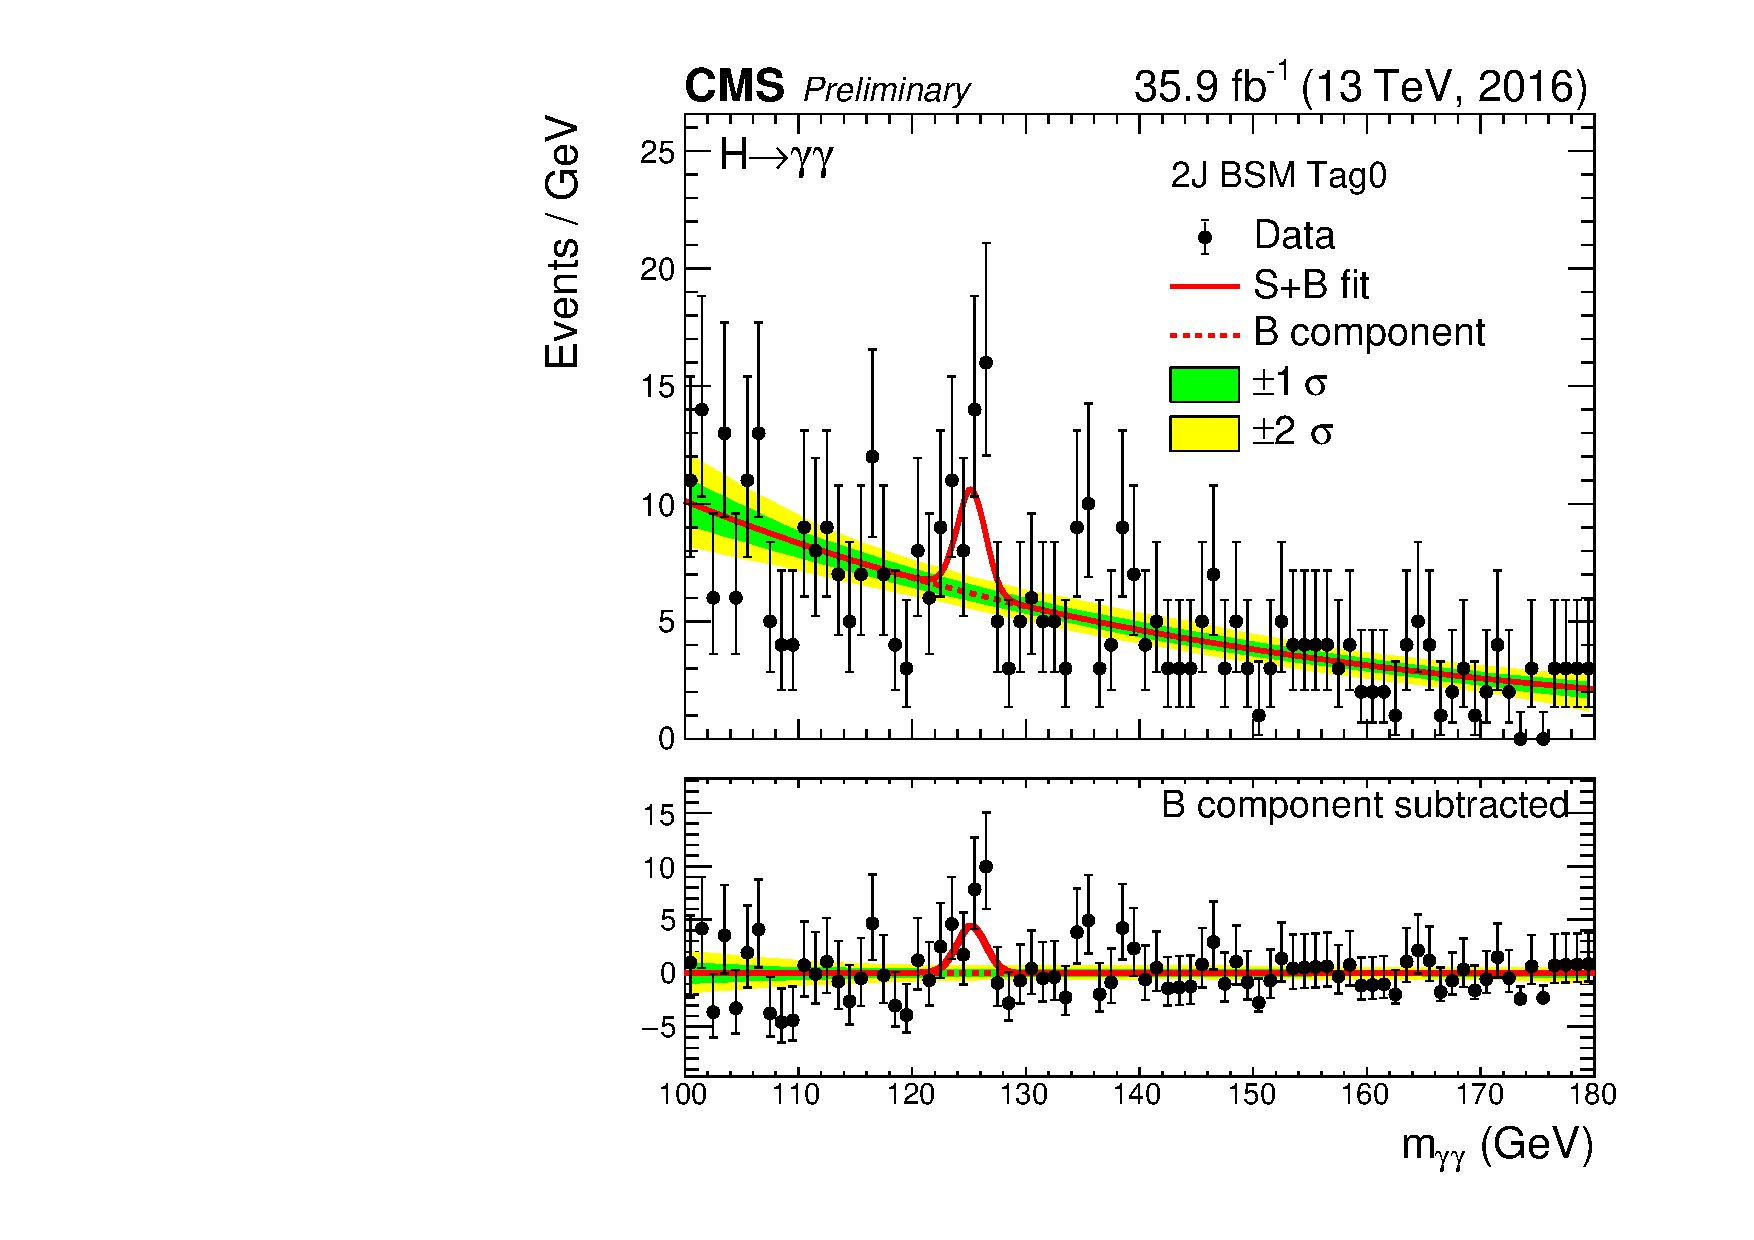
\includegraphics[width=0.49\textwidth]{Figures/Appendices/_forAppendix2016ch1_RECO_GE2J_PTH_GT200_Tag0_13TeV.pdf}
  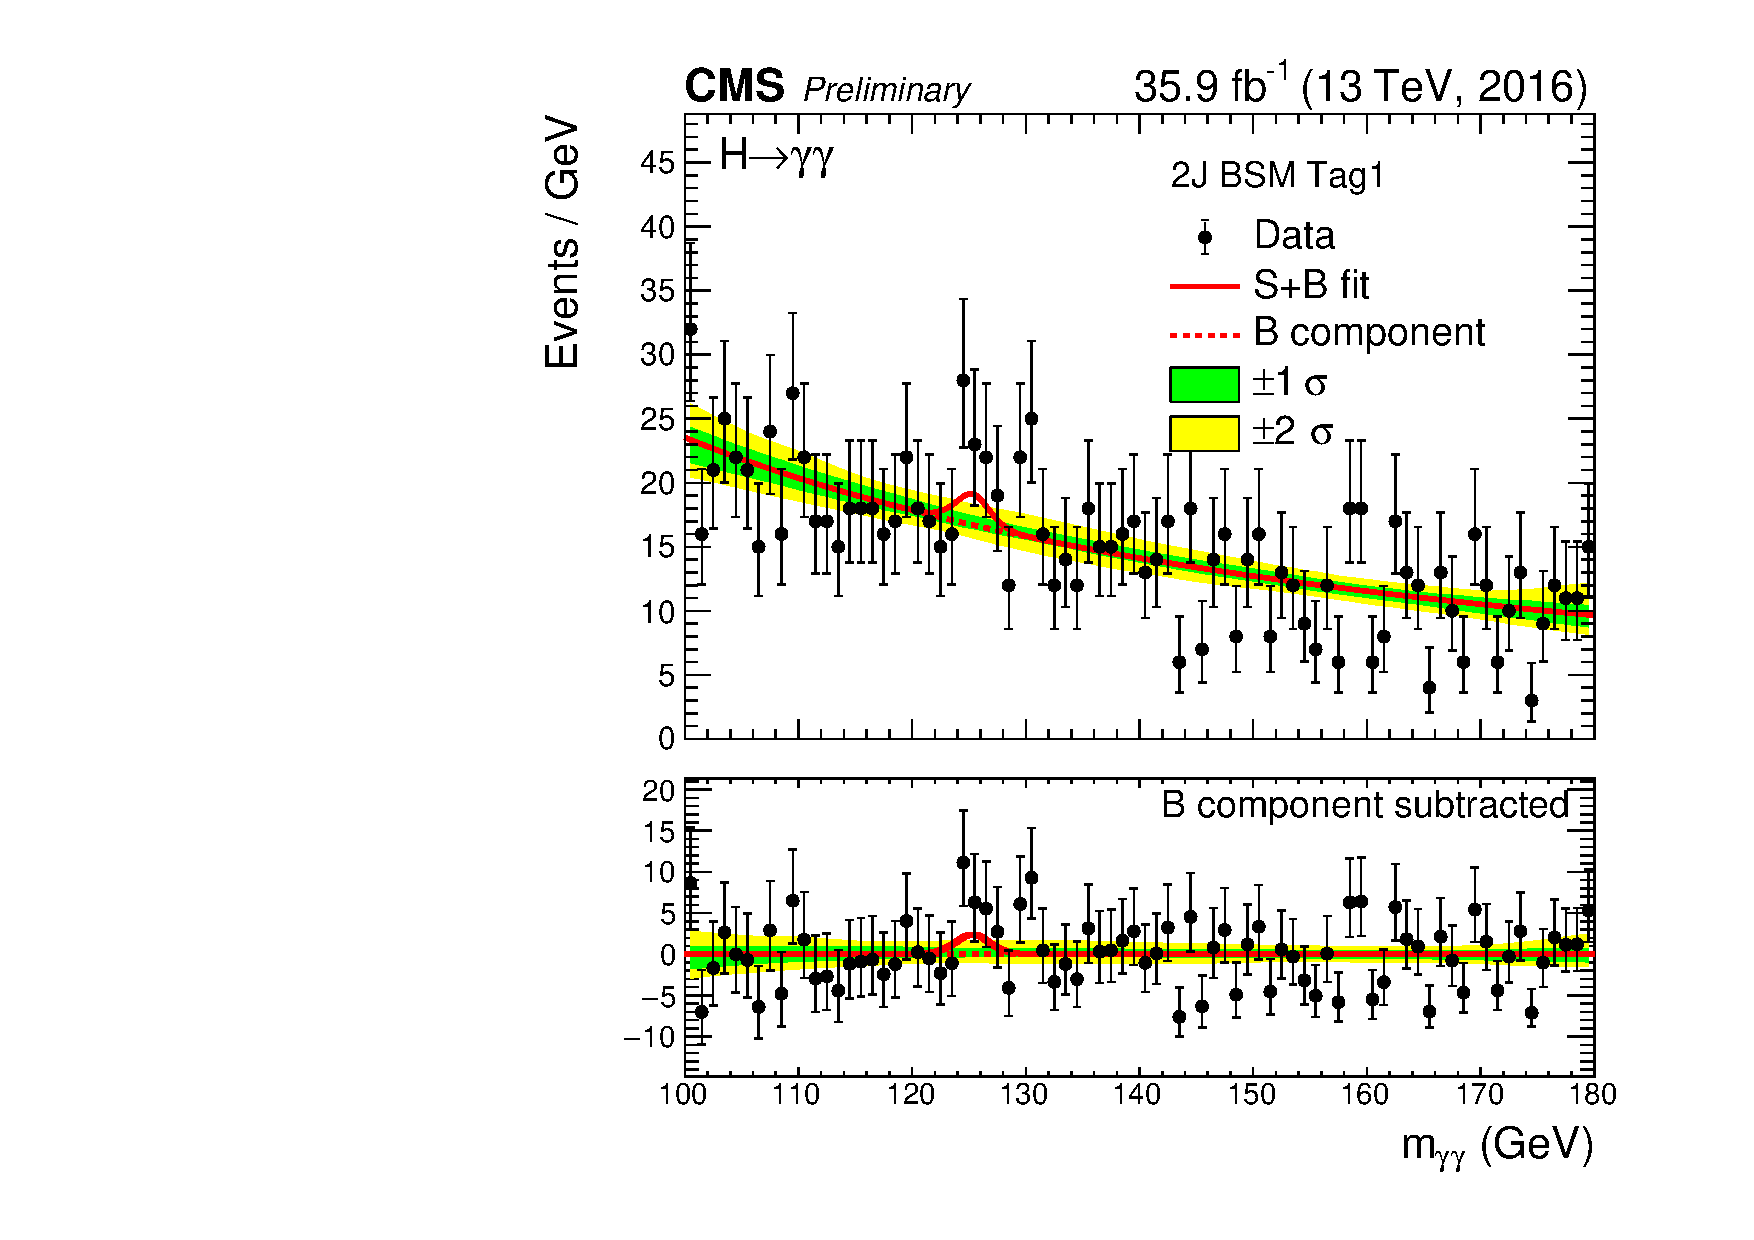
\includegraphics[width=0.49\textwidth]{Figures/Appendices/_forAppendix2016ch1_RECO_GE2J_PTH_GT200_Tag1_13TeV.pdf}
  \caption[Signal plus background fits to data.]
  {
    Data points (black) and signal plus background model fit are shown. 
    The one standard deviation (green) and two standard deviation (yellow) bands 
    include the uncertainties in the background component of the fit. 
    The solid red line shows the contribution from the total signal, plus the background contribution. 
    The dashed red line shows the contribution from the background component of the fit. 
    The bottom plot shows the residuals after subtraction of this background component.
  }
\end{figure}

\begin{figure}[hptb]
  \centering
  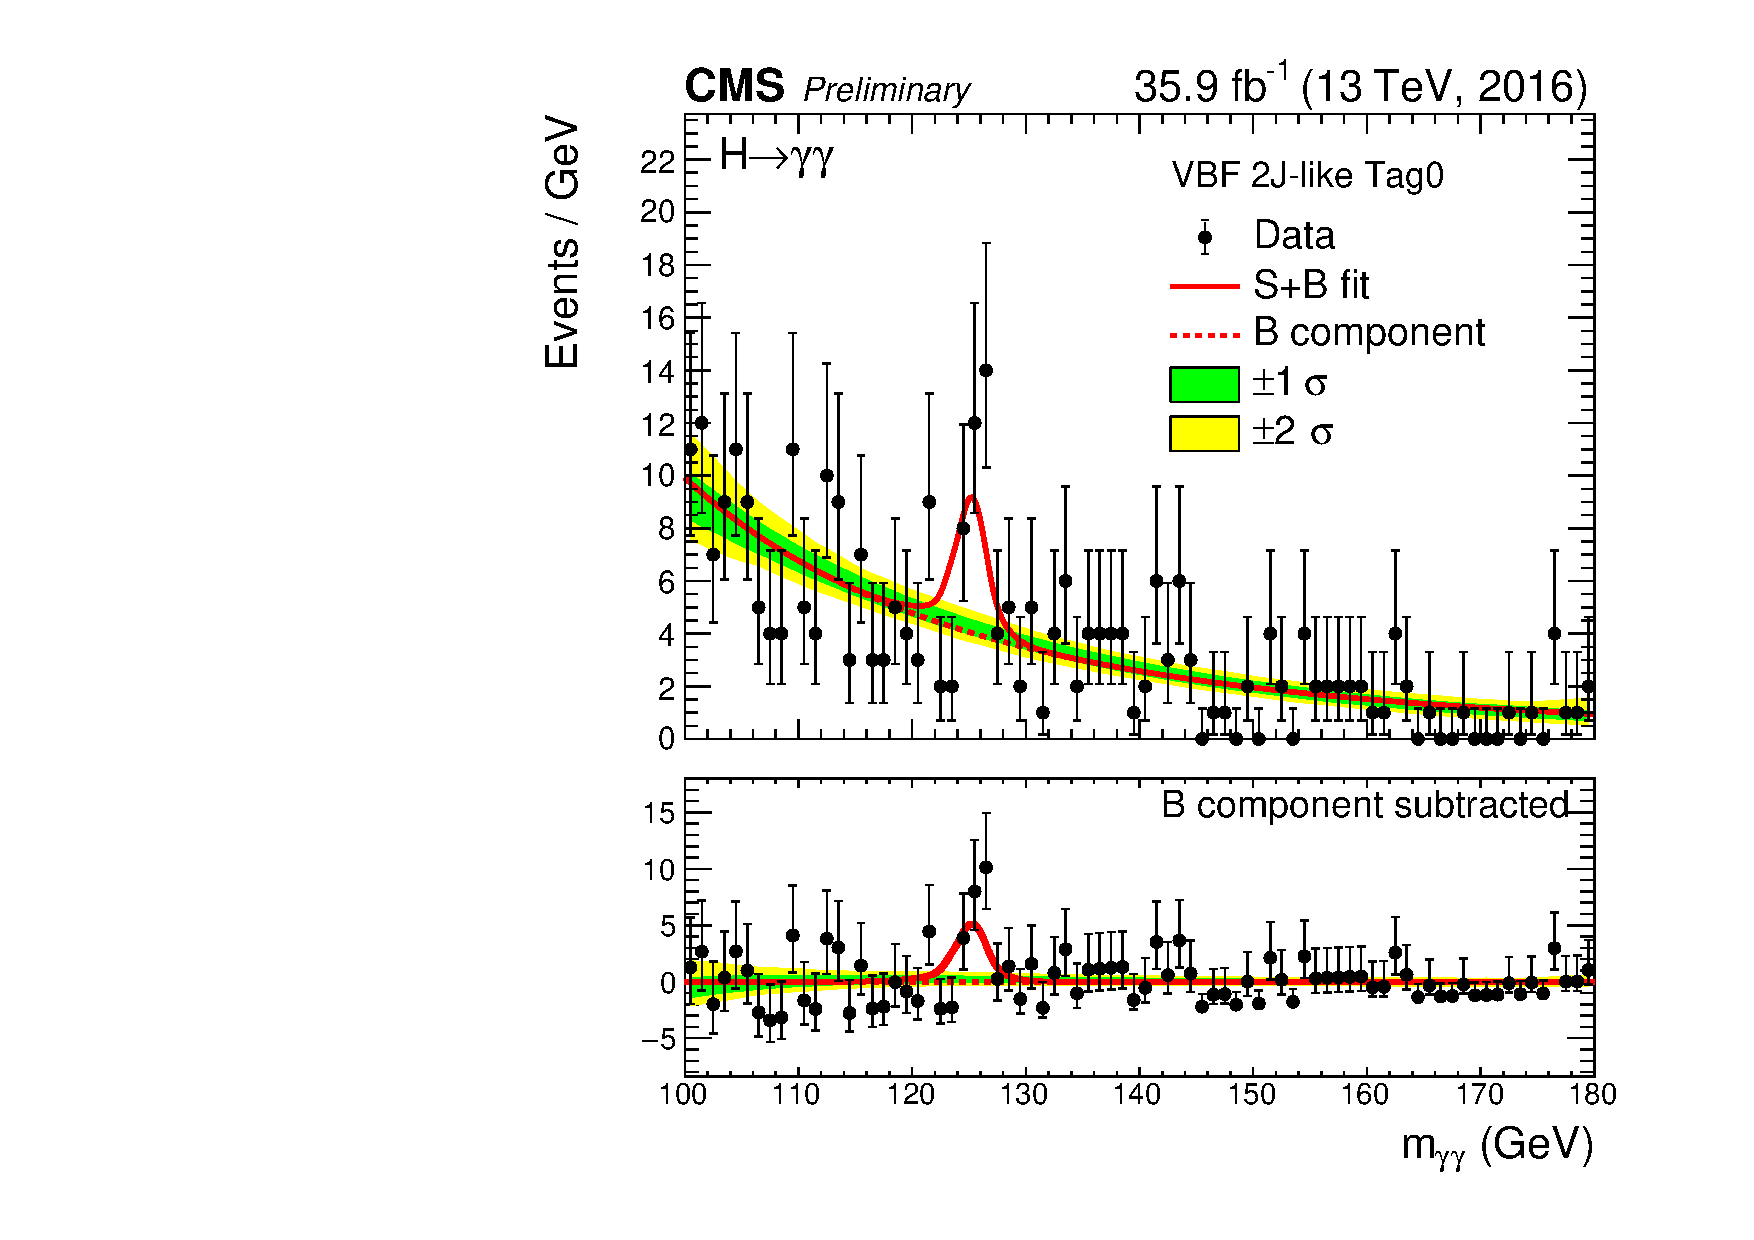
\includegraphics[width=0.49\textwidth]{Figures/Appendices/_forAppendix2016ch1_RECO_VBFTOPO_JET3VETO_Tag0_13TeV.pdf}
  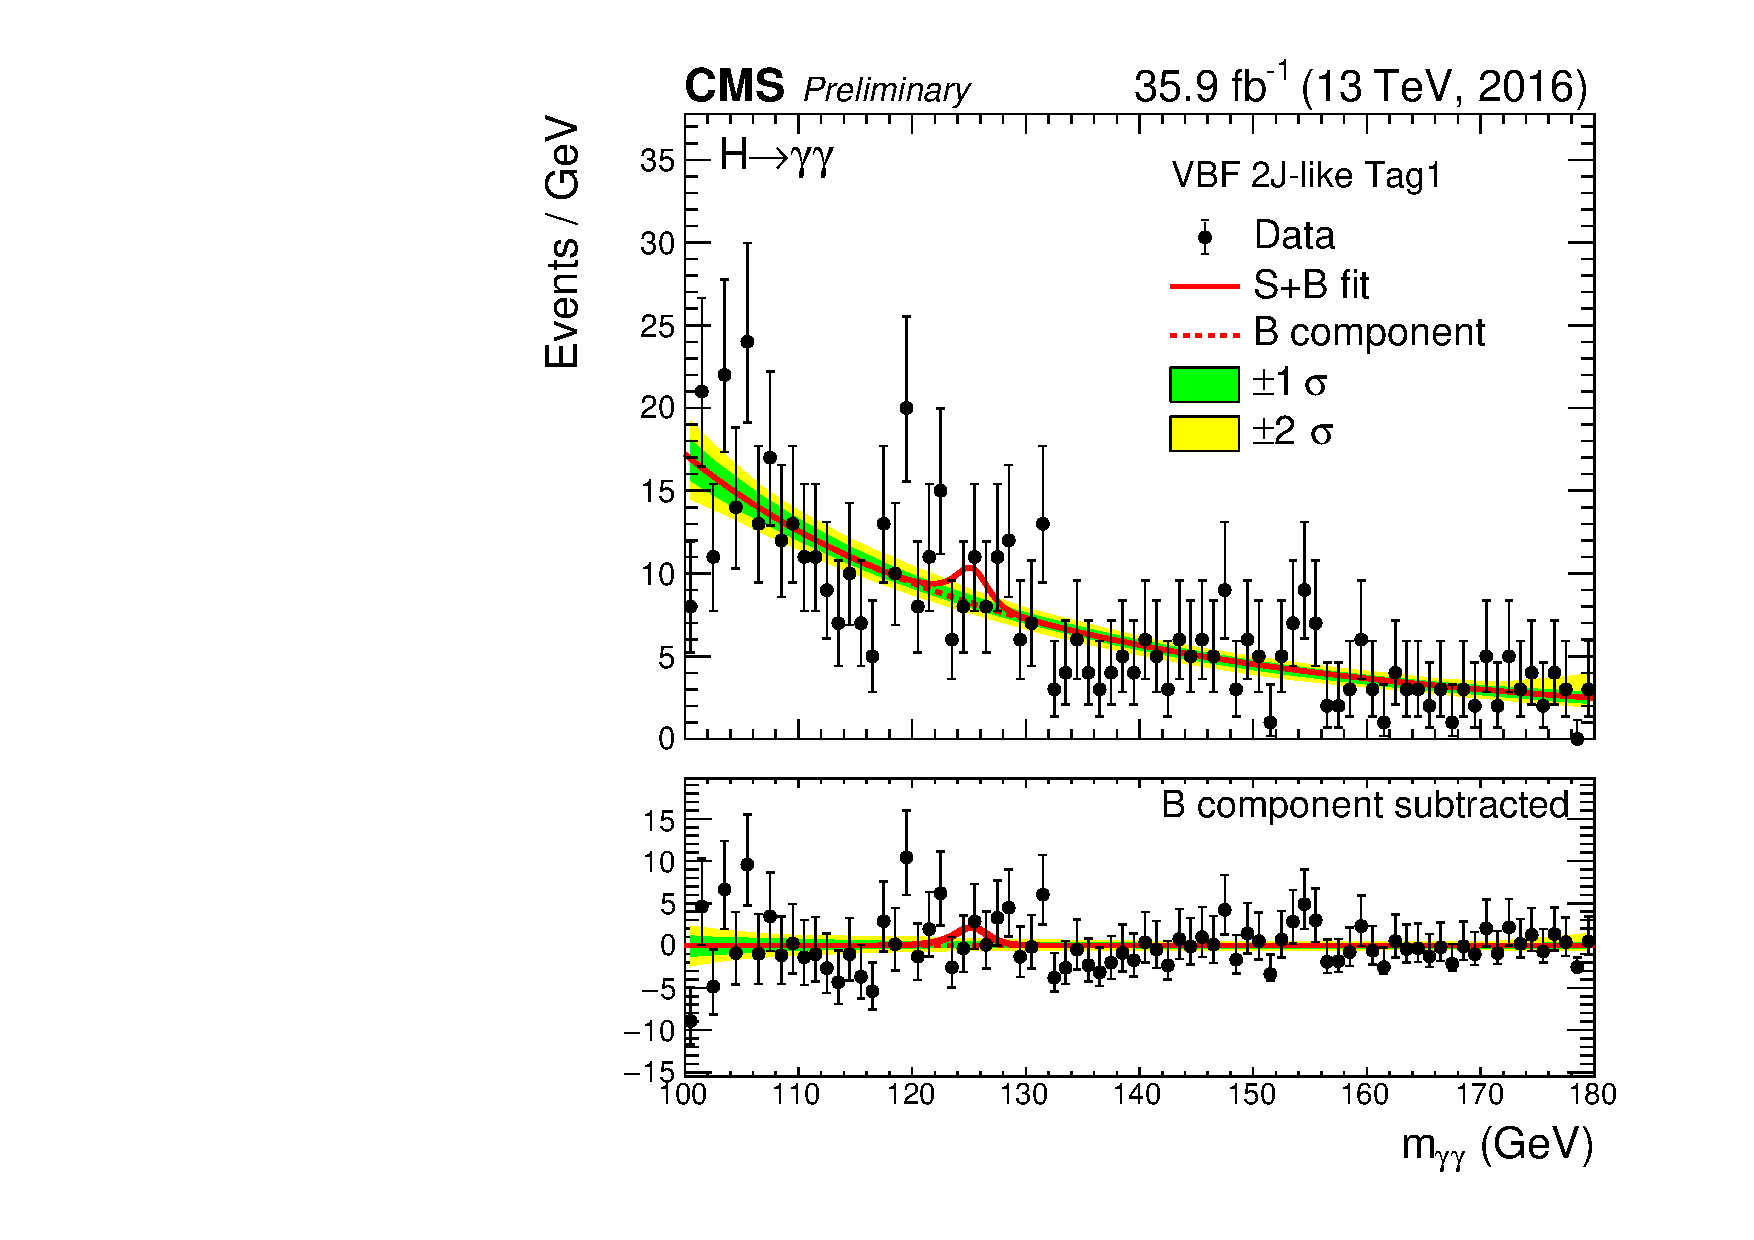
\includegraphics[width=0.49\textwidth]{Figures/Appendices/_forAppendix2016ch1_RECO_VBFTOPO_JET3VETO_Tag1_13TeV.pdf}
  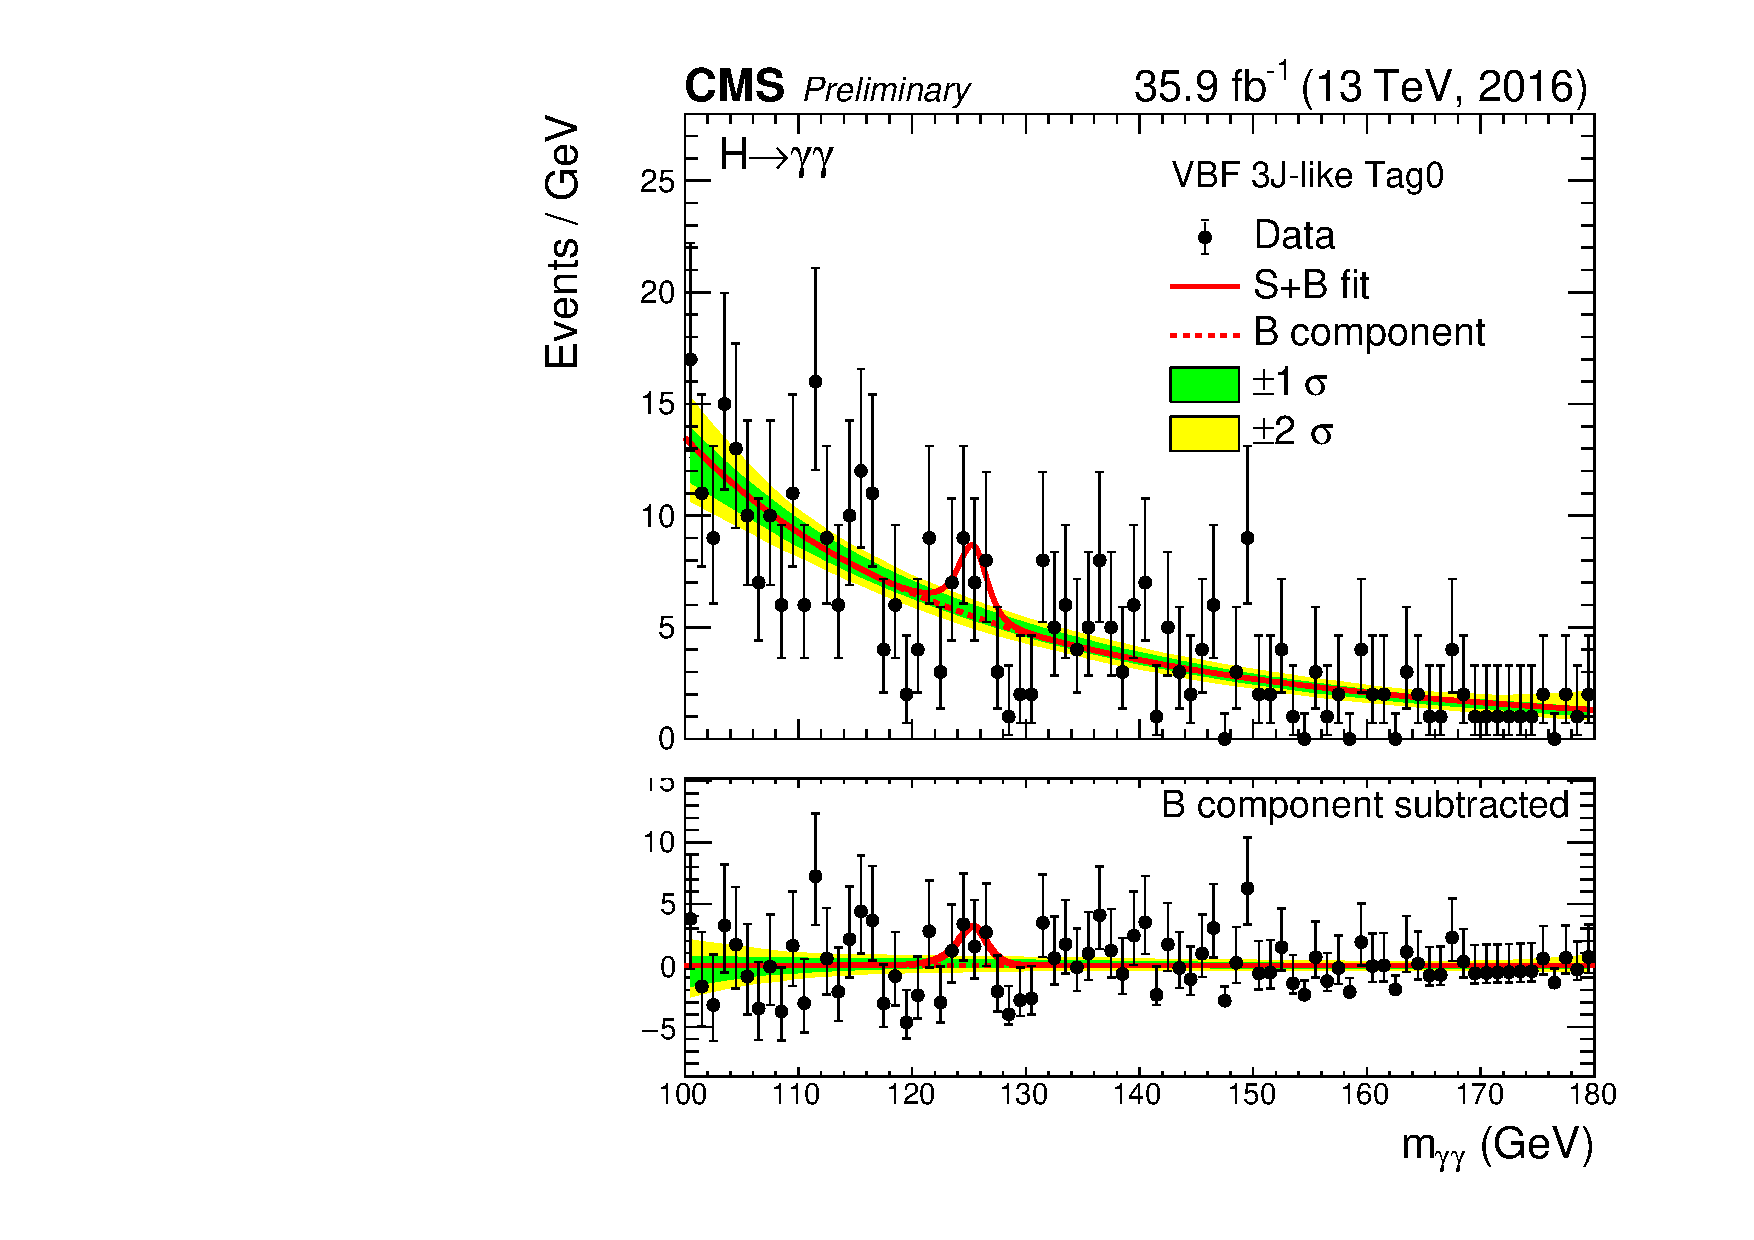
\includegraphics[width=0.49\textwidth]{Figures/Appendices/_forAppendix2016ch1_RECO_VBFTOPO_JET3_Tag0_13TeV.pdf}
  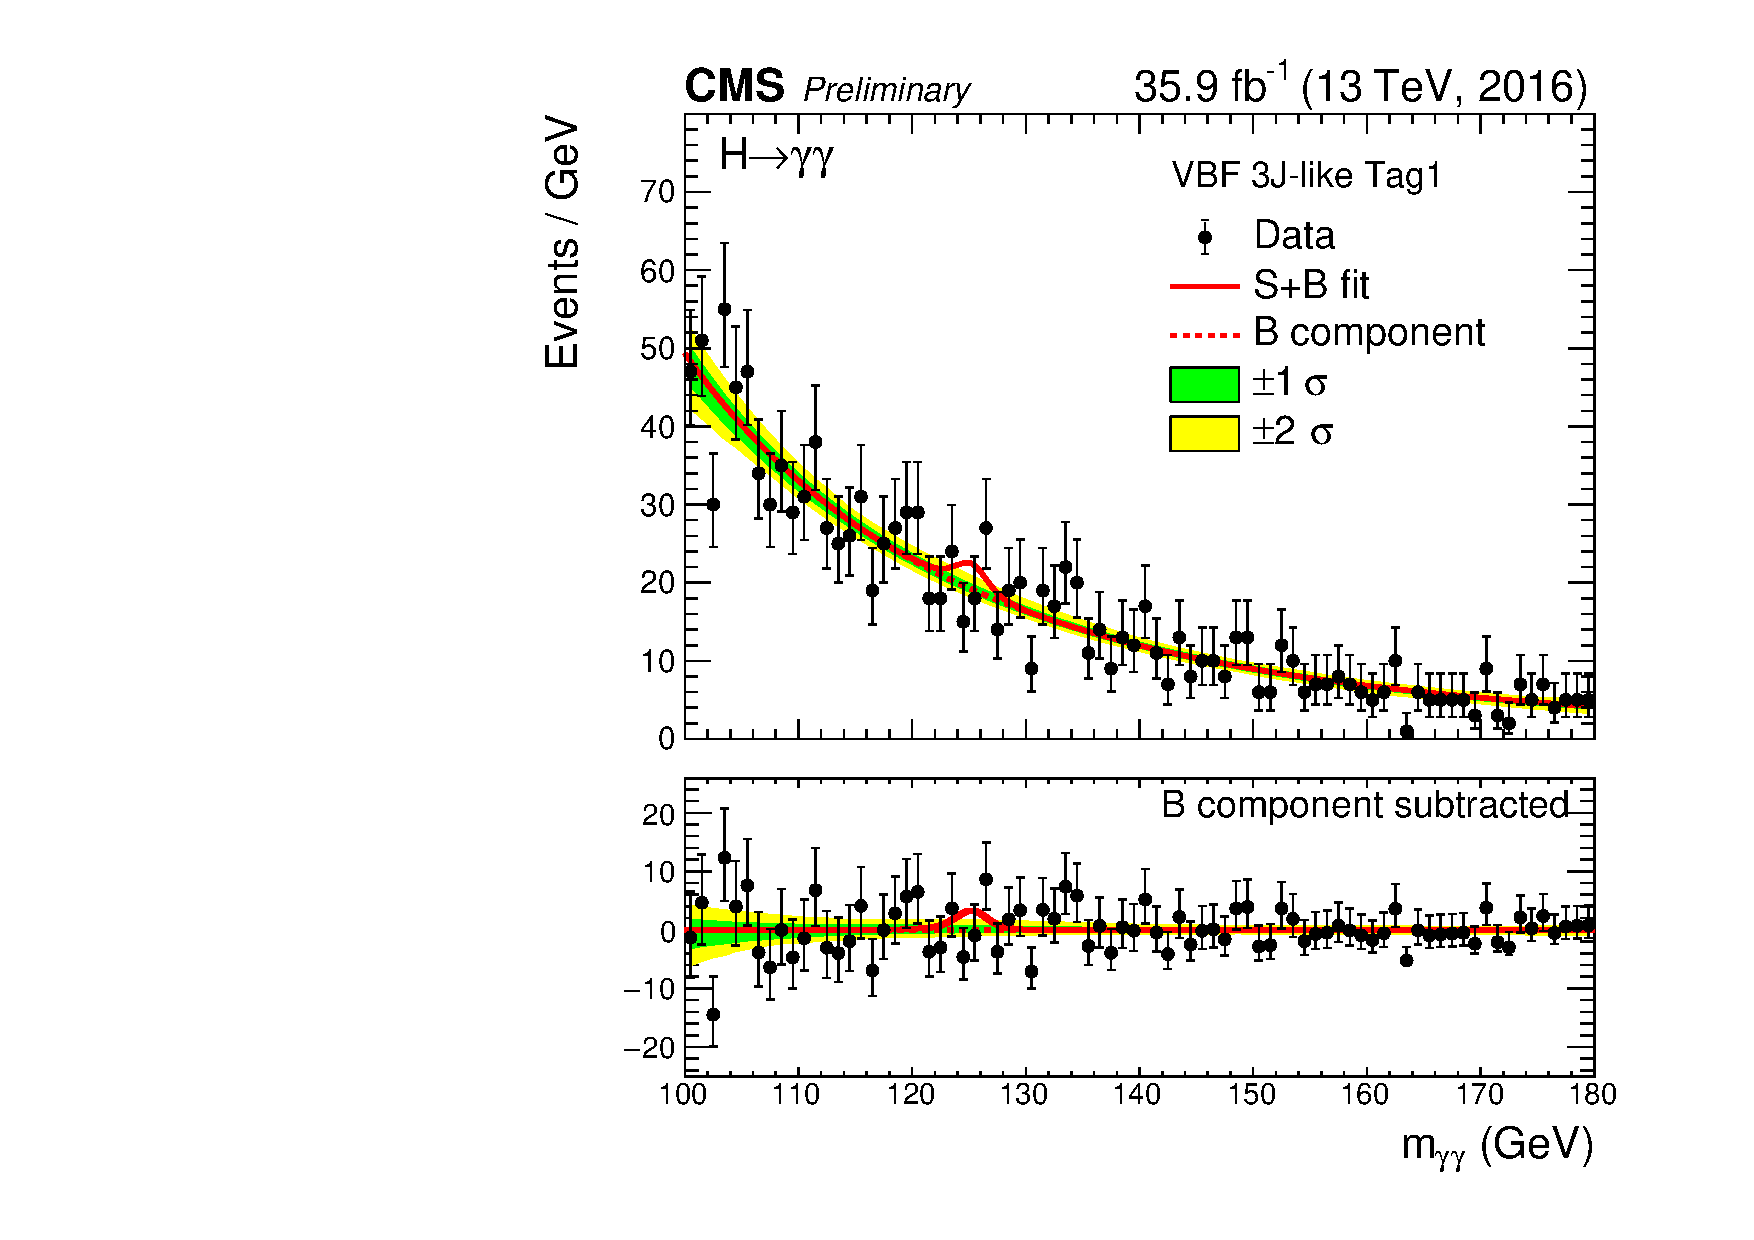
\includegraphics[width=0.49\textwidth]{Figures/Appendices/_forAppendix2016ch1_RECO_VBFTOPO_JET3_Tag1_13TeV.pdf}
  \caption[Signal plus background fits to data.]
  {
    Data points (black) and signal plus background model fit are shown. 
    The one standard deviation (green) and two standard deviation (yellow) bands 
    include the uncertainties in the background component of the fit. 
    The solid red line shows the contribution from the total signal, plus the background contribution. 
    The dashed red line shows the contribution from the background component of the fit. 
    The bottom plot shows the residuals after subtraction of this background component.
  }
\end{figure}

\begin{figure}[hptb]
  \centering
  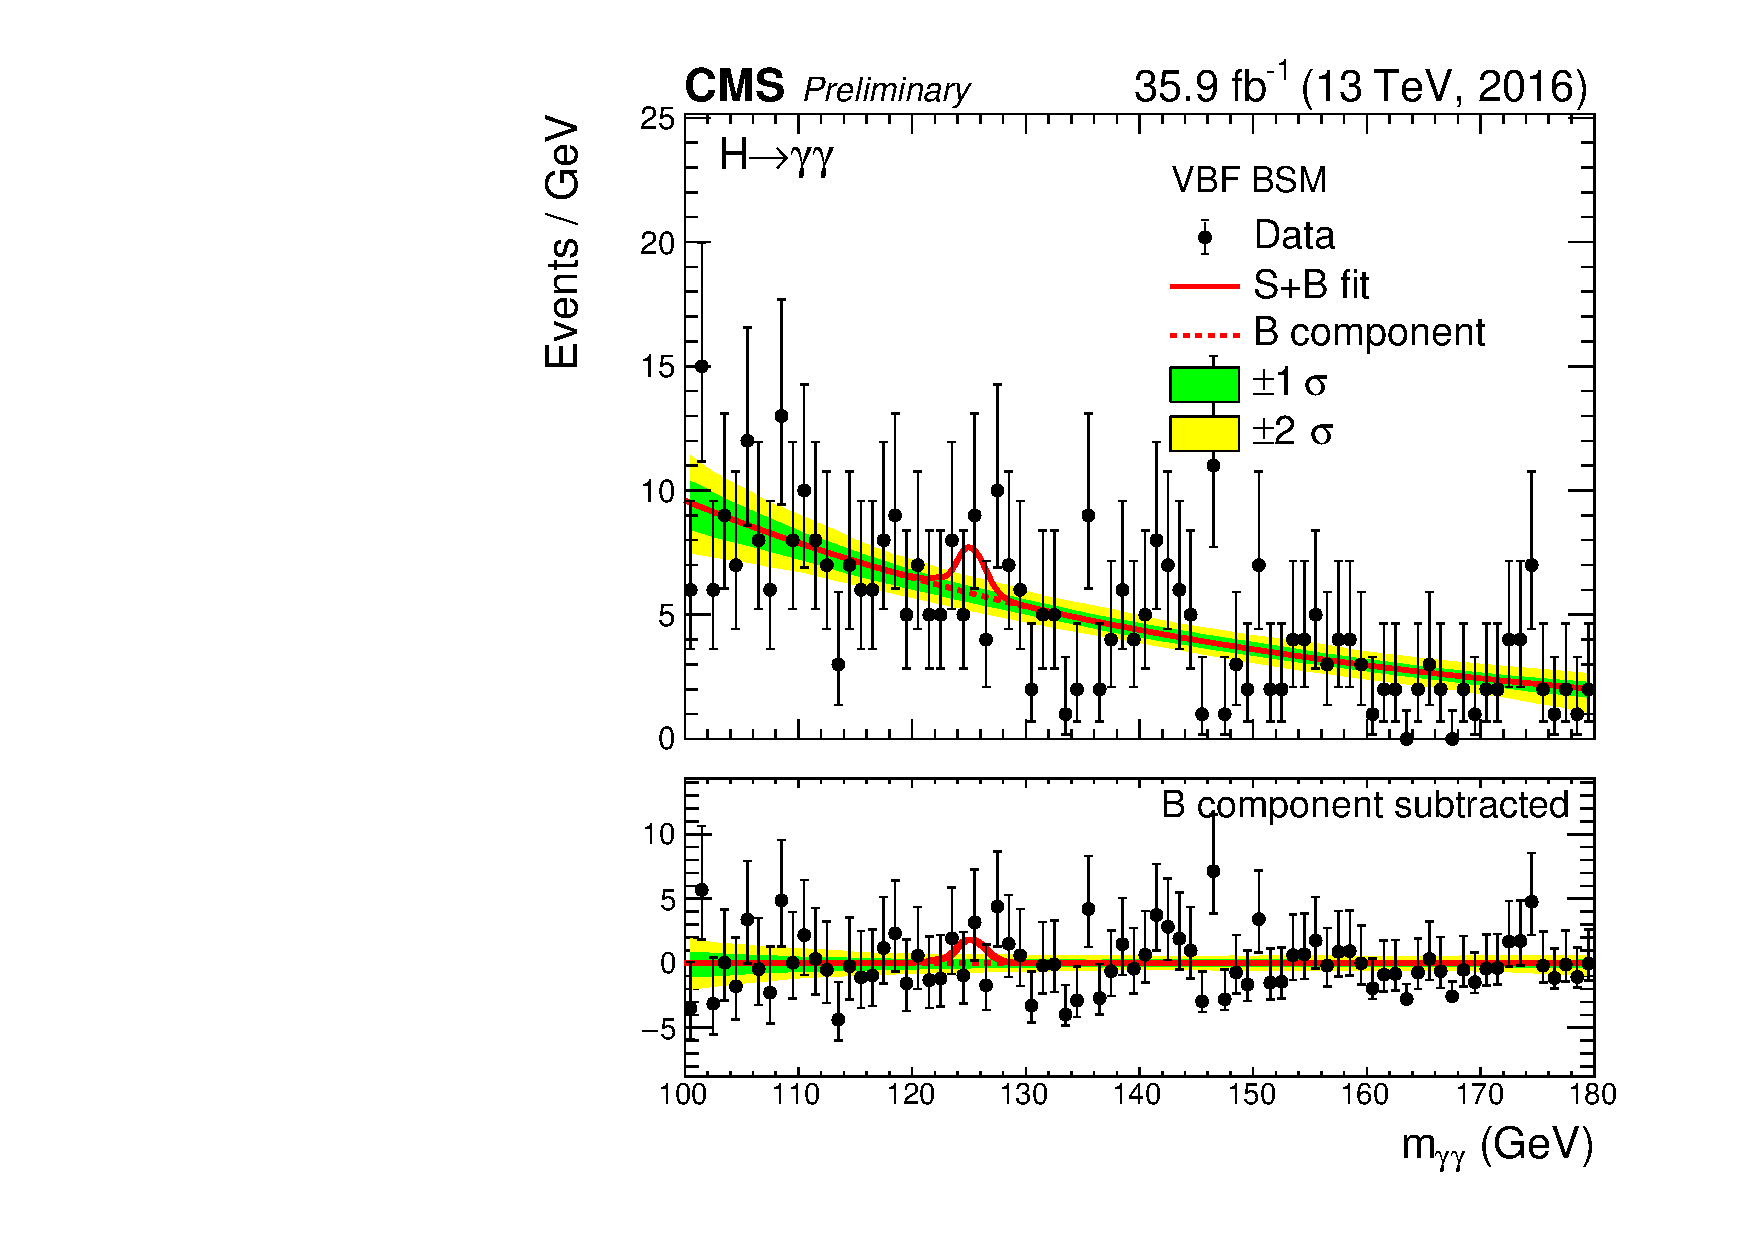
\includegraphics[width=0.49\textwidth]{Figures/Appendices/_forAppendix2016ch1_RECO_VBFTOPO_BSM_13TeV.pdf}
  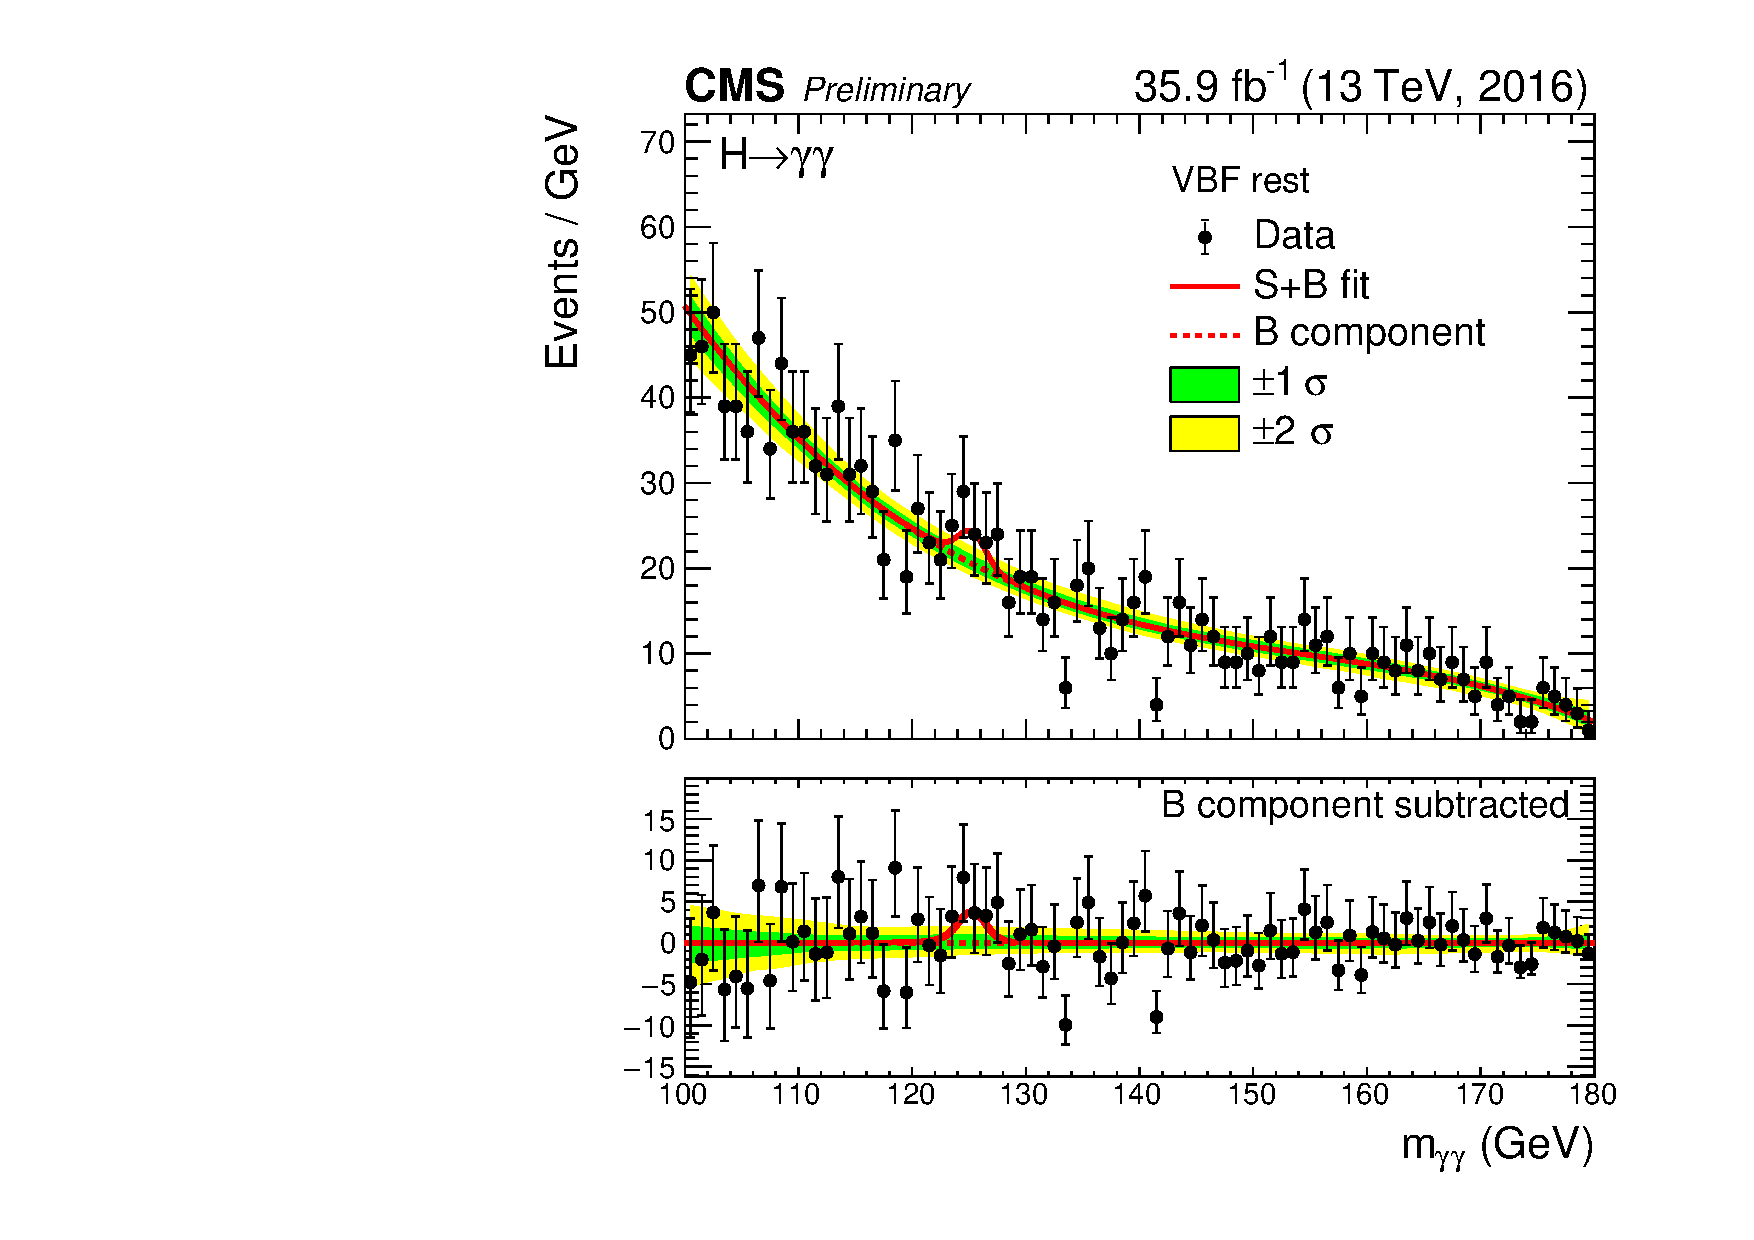
\includegraphics[width=0.49\textwidth]{Figures/Appendices/_forAppendix2016ch1_RECO_VBFTOPO_REST_13TeV.pdf}
  \caption[Signal plus background fits to data.]
  {
    Data points (black) and signal plus background model fit are shown. 
    The one standard deviation (green) and two standard deviation (yellow) bands 
    include the uncertainties in the background component of the fit. 
    The solid red line shows the contribution from the total signal, plus the background contribution. 
    The dashed red line shows the contribution from the background component of the fit. 
    The bottom plot shows the residuals after subtraction of this background component.
  }
\end{figure}

\begin{figure}[hptb]
  \centering
  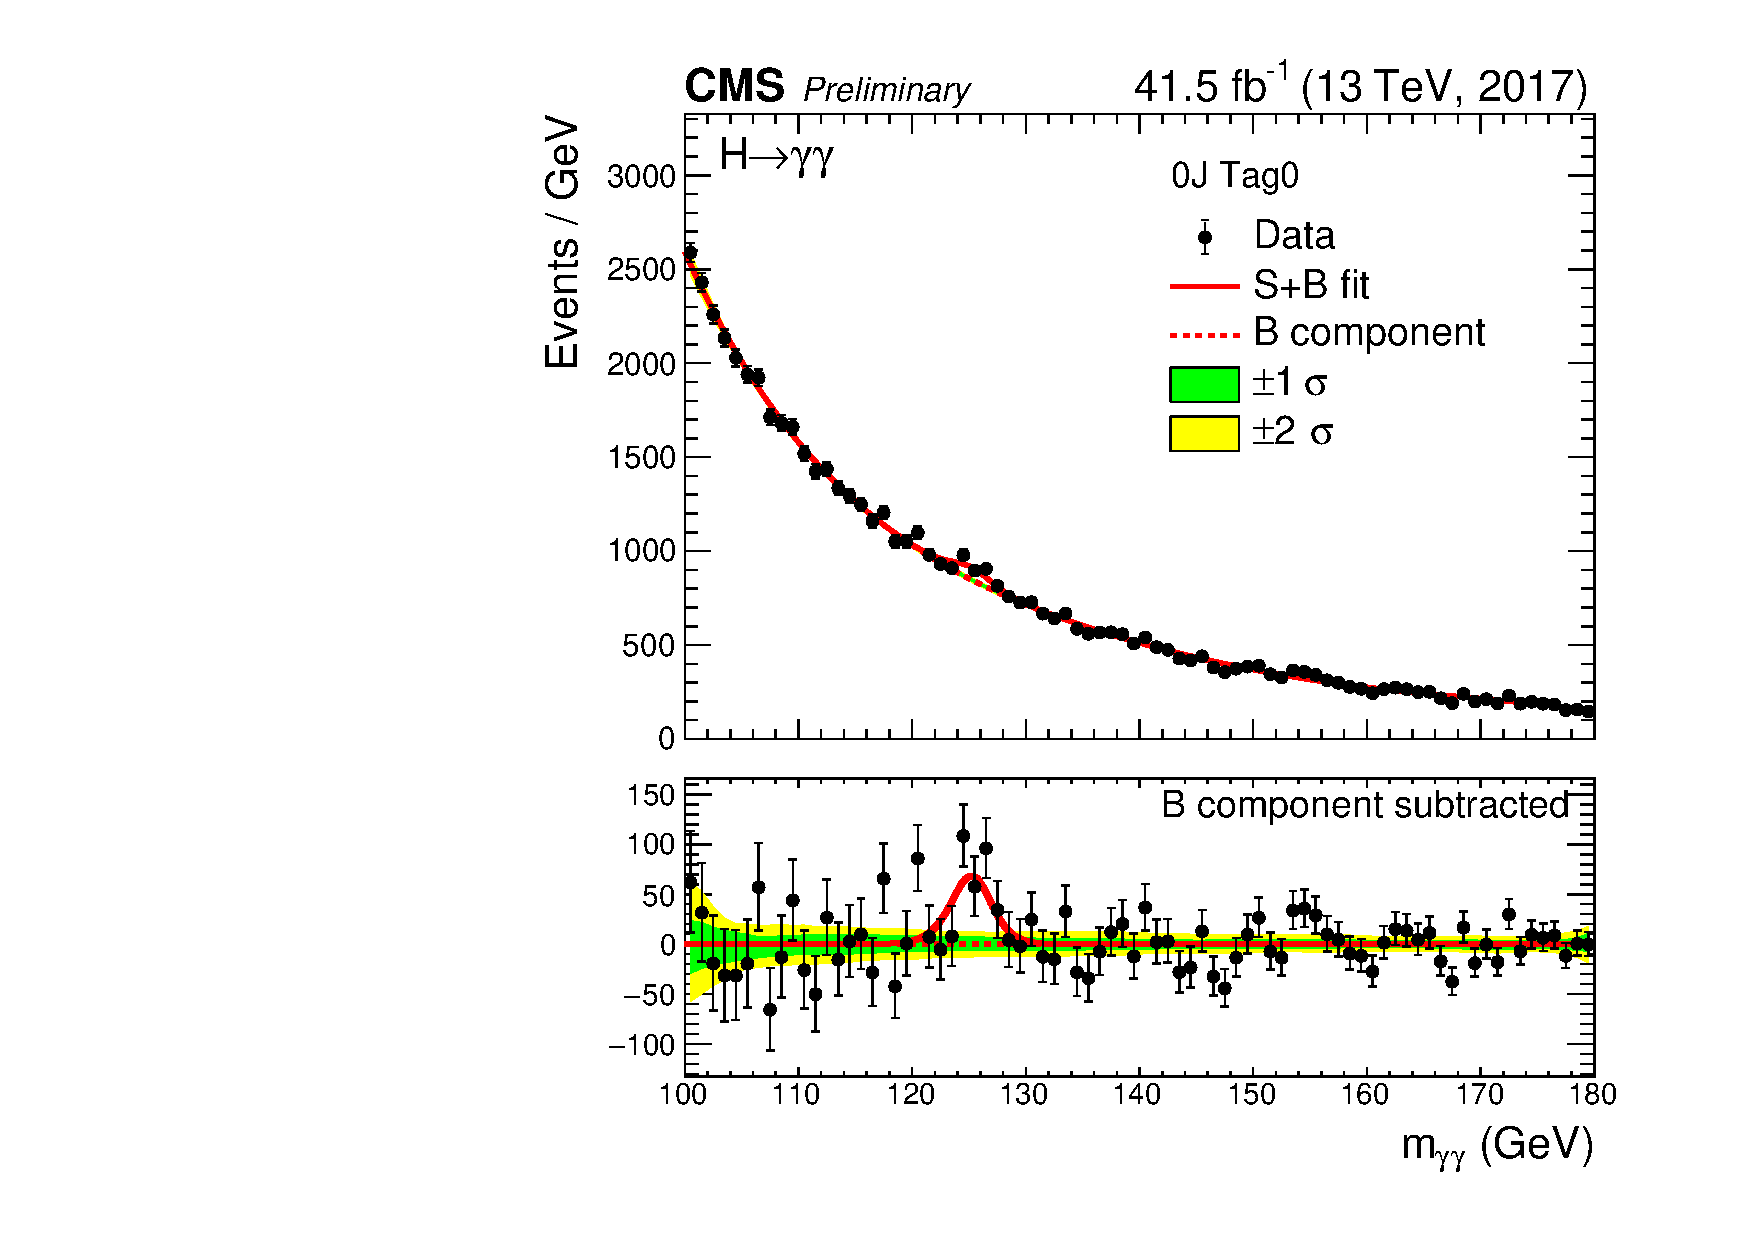
\includegraphics[width=0.49\textwidth]{Figures/Appendices/_forAppendix2017ch2_RECO_0J_Tag0_13TeV.pdf}
  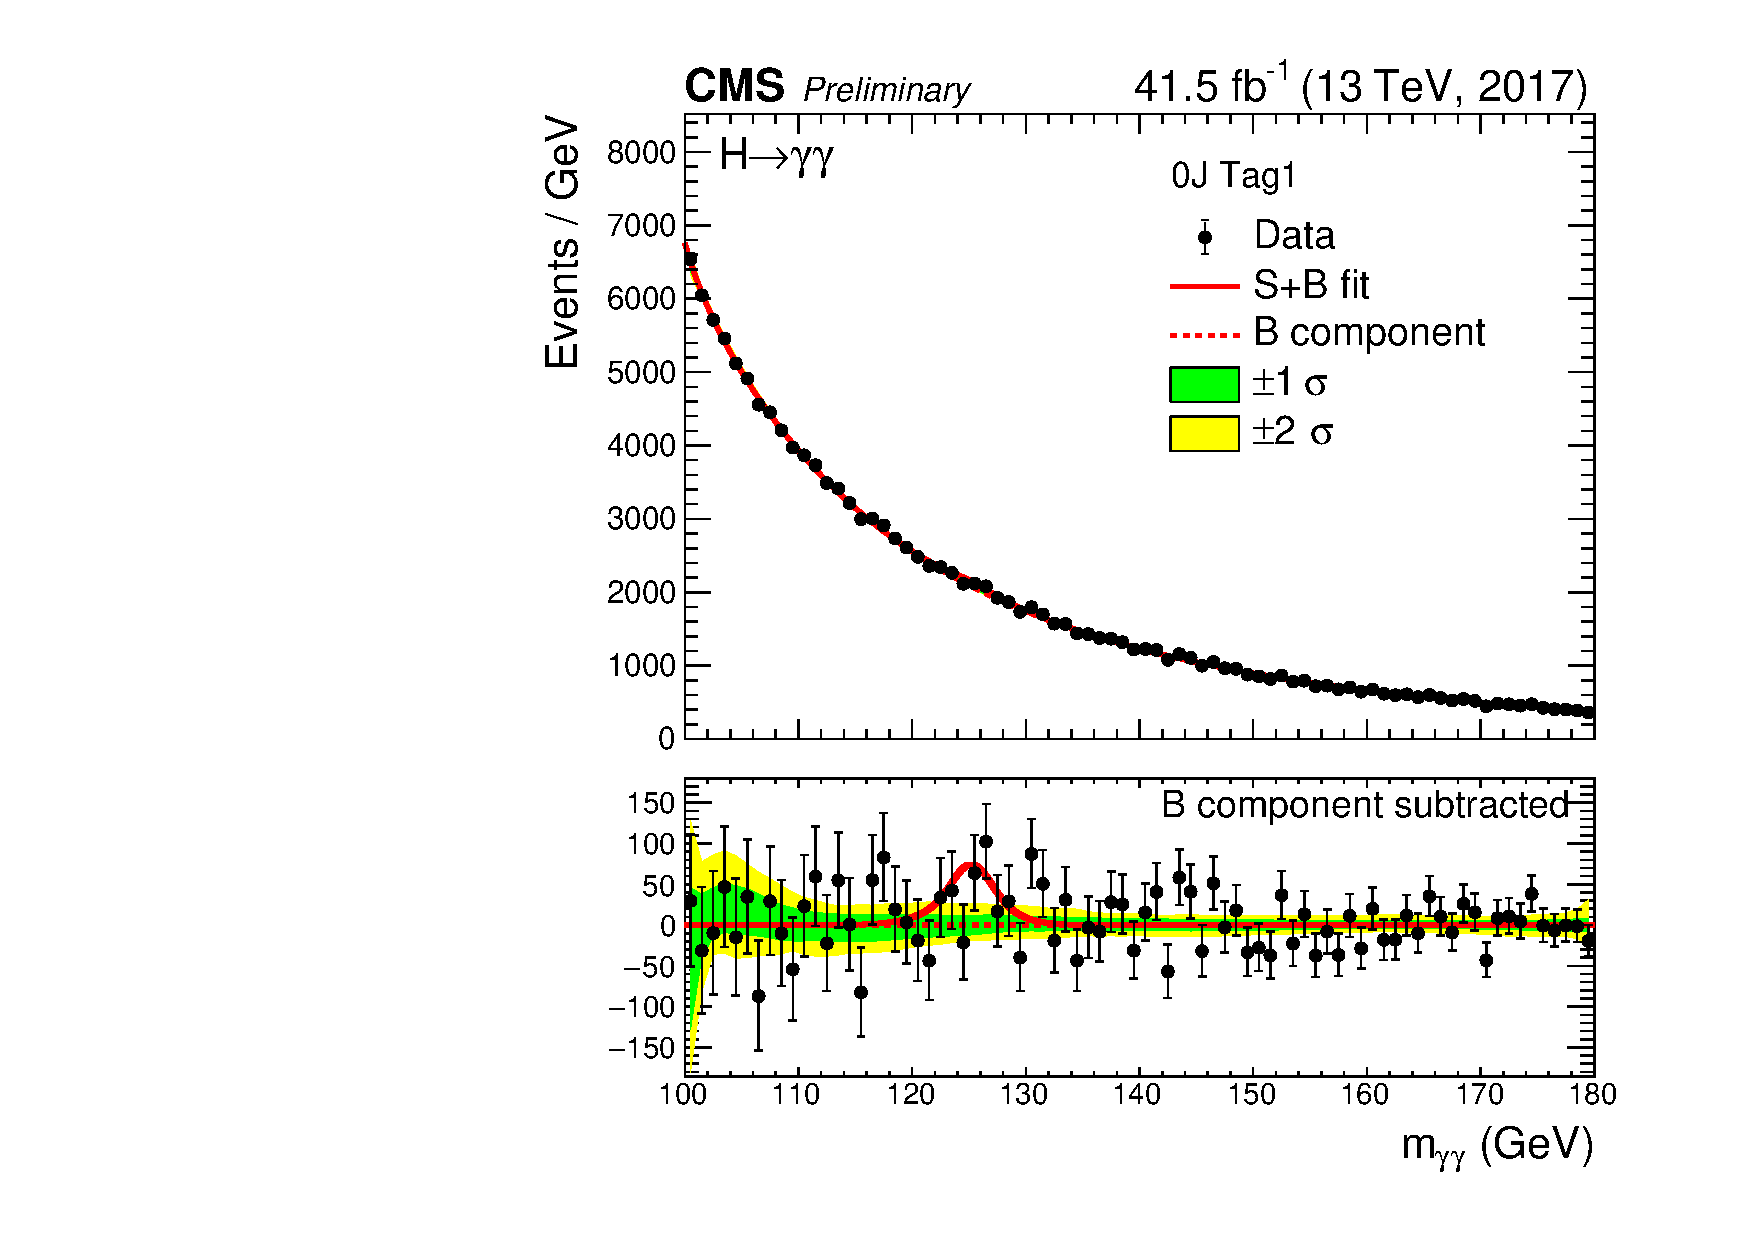
\includegraphics[width=0.49\textwidth]{Figures/Appendices/_forAppendix2017ch2_RECO_0J_Tag1_13TeV.pdf}
  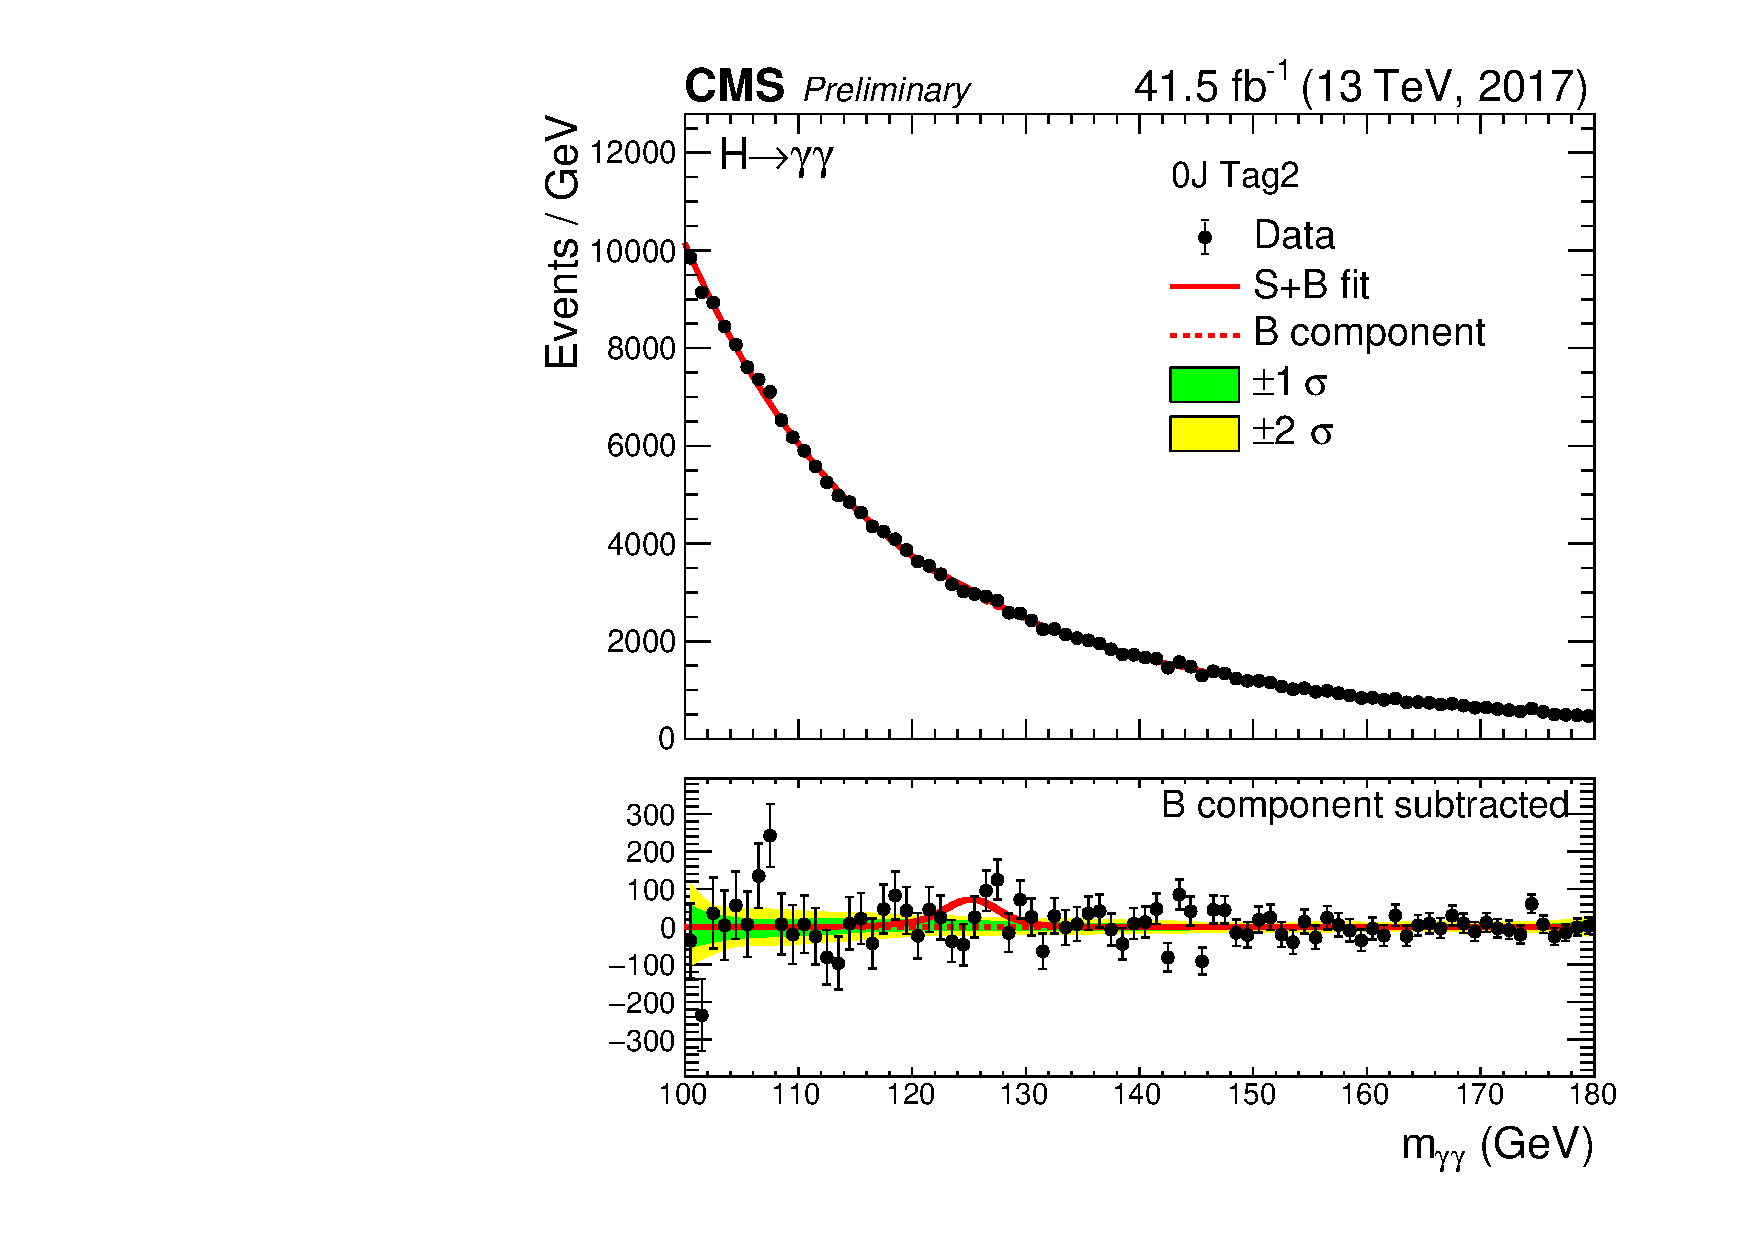
\includegraphics[width=0.49\textwidth]{Figures/Appendices/_forAppendix2017ch2_RECO_0J_Tag2_13TeV.pdf}
  \caption[Signal plus background fits to data.]
  {
    Data points (black) and signal plus background model fit are shown. 
    The one standard deviation (green) and two standard deviation (yellow) bands 
    include the uncertainties in the background component of the fit. 
    The solid red line shows the contribution from the total signal, plus the background contribution. 
    The dashed red line shows the contribution from the background component of the fit. 
    The bottom plot shows the residuals after subtraction of this background component.
  }
\end{figure}

\begin{figure}[hptb]
  \centering
  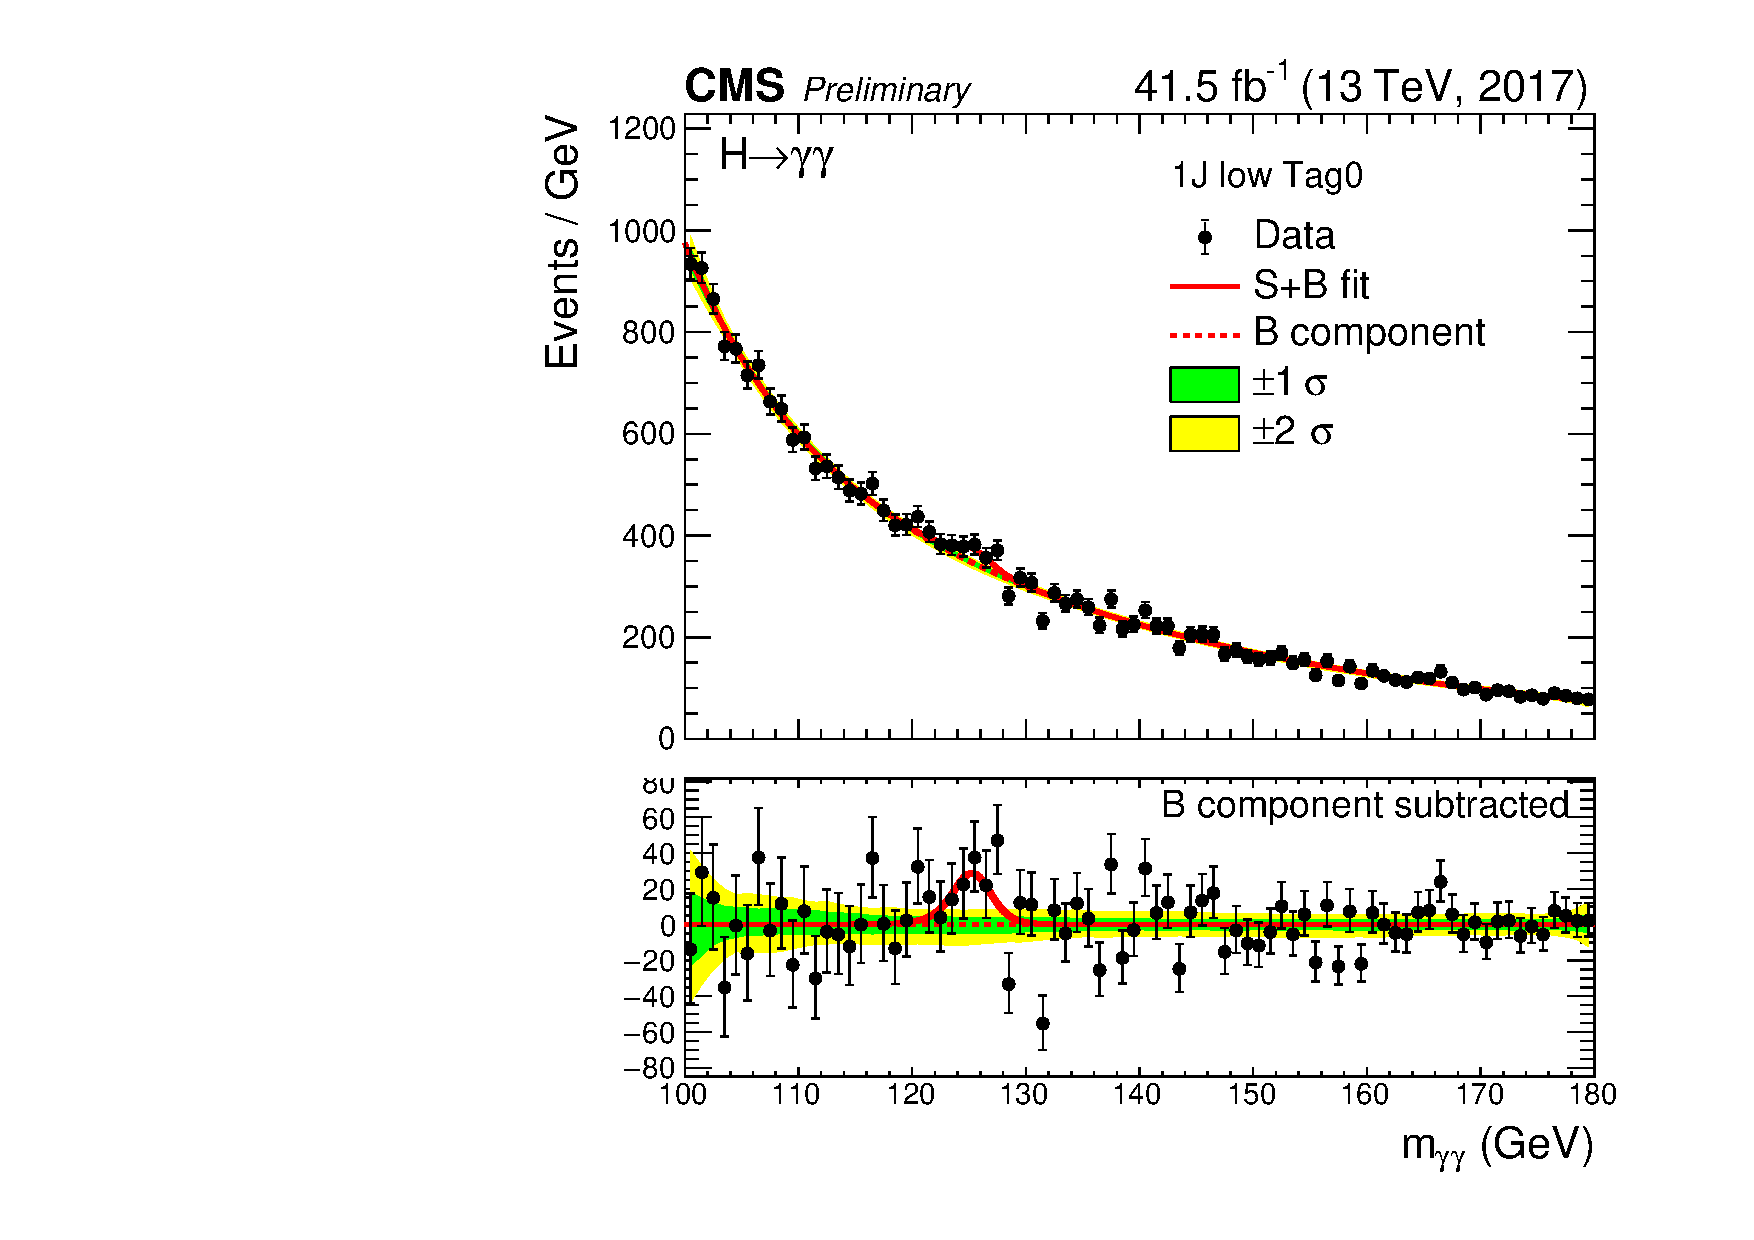
\includegraphics[width=0.49\textwidth]{Figures/Appendices/_forAppendix2017ch2_RECO_1J_PTH_0_60_Tag0_13TeV.pdf}
  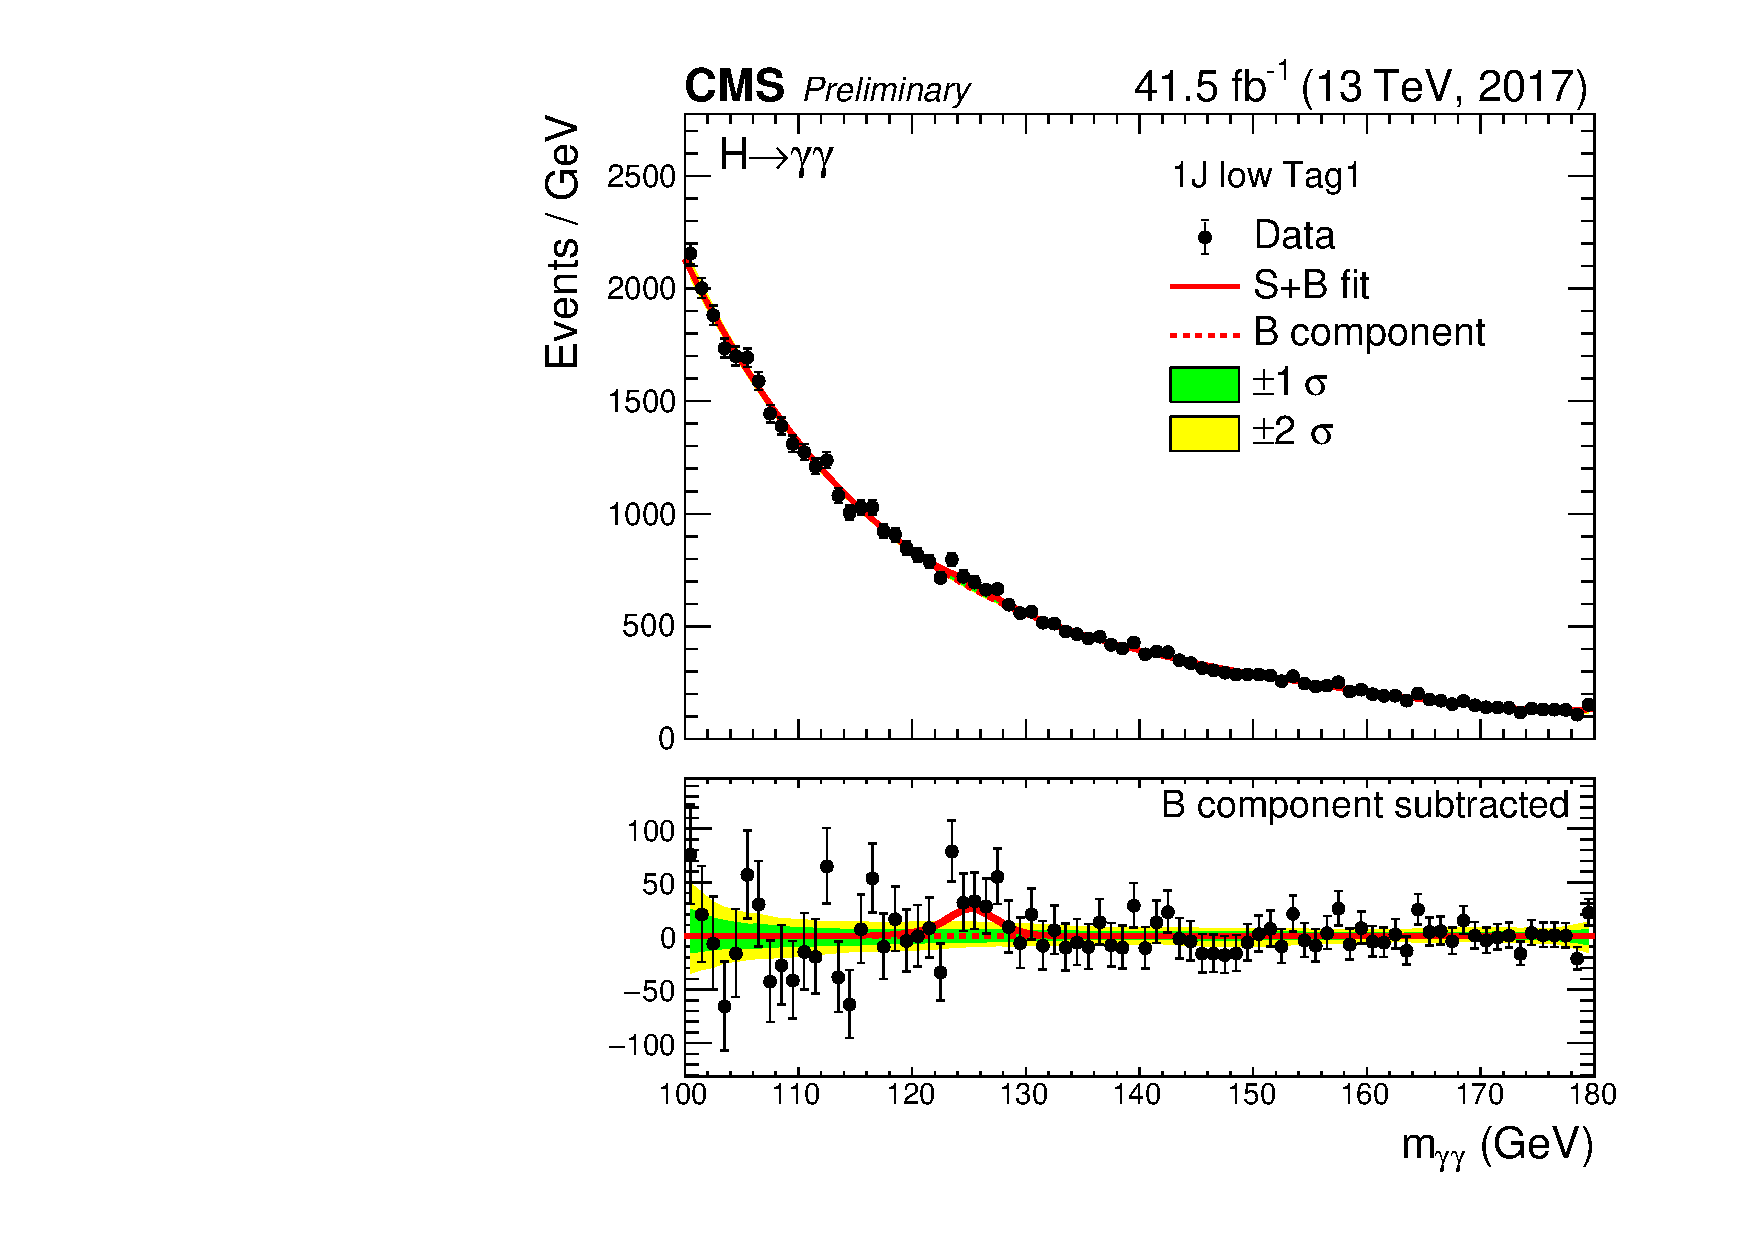
\includegraphics[width=0.49\textwidth]{Figures/Appendices/_forAppendix2017ch2_RECO_1J_PTH_0_60_Tag1_13TeV.pdf}
  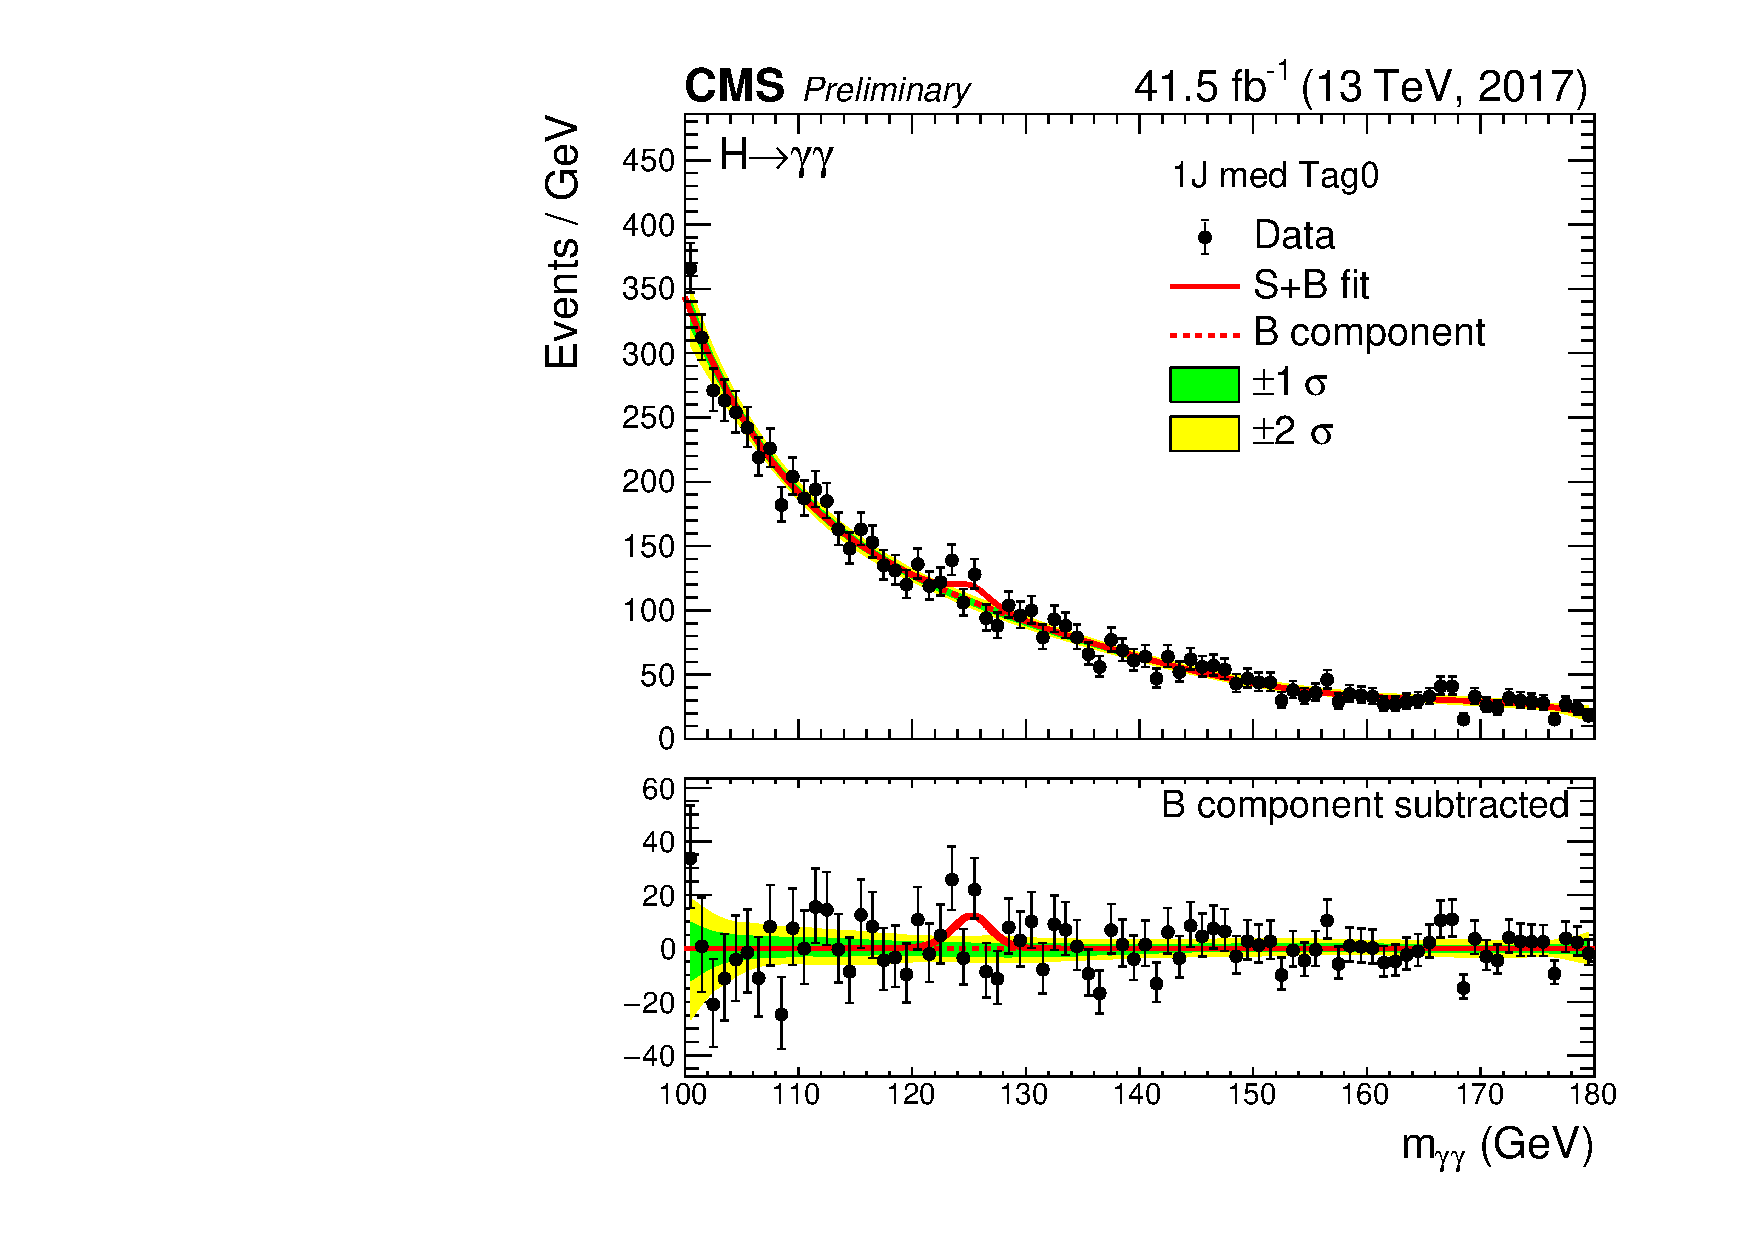
\includegraphics[width=0.49\textwidth]{Figures/Appendices/_forAppendix2017ch2_RECO_1J_PTH_60_120_Tag0_13TeV.pdf}
  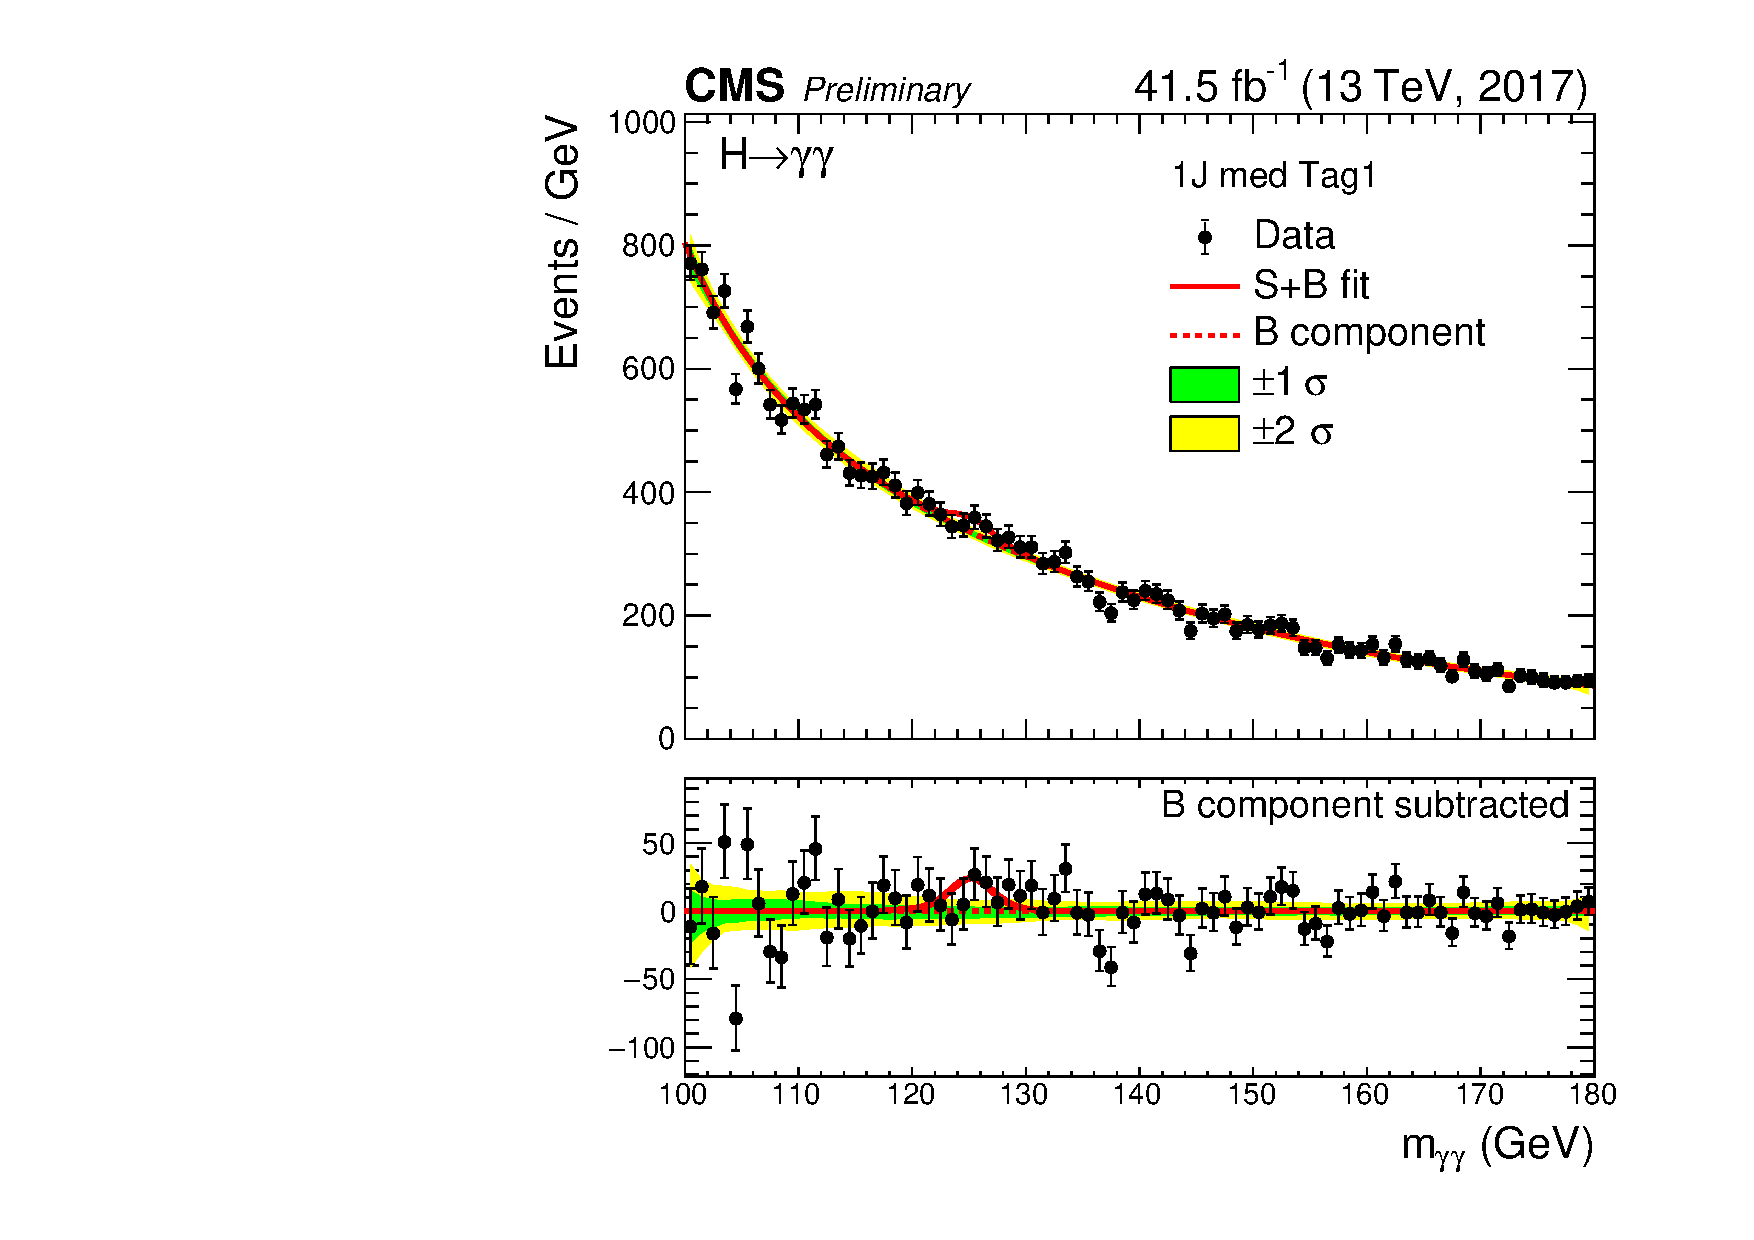
\includegraphics[width=0.49\textwidth]{Figures/Appendices/_forAppendix2017ch2_RECO_1J_PTH_60_120_Tag1_13TeV.pdf}
  \caption[Signal plus background fits to data.]
  {
    Data points (black) and signal plus background model fit are shown. 
    The one standard deviation (green) and two standard deviation (yellow) bands 
    include the uncertainties in the background component of the fit. 
    The solid red line shows the contribution from the total signal, plus the background contribution. 
    The dashed red line shows the contribution from the background component of the fit. 
    The bottom plot shows the residuals after subtraction of this background component.
  }
\end{figure}

\begin{figure}[hptb]
  \centering
  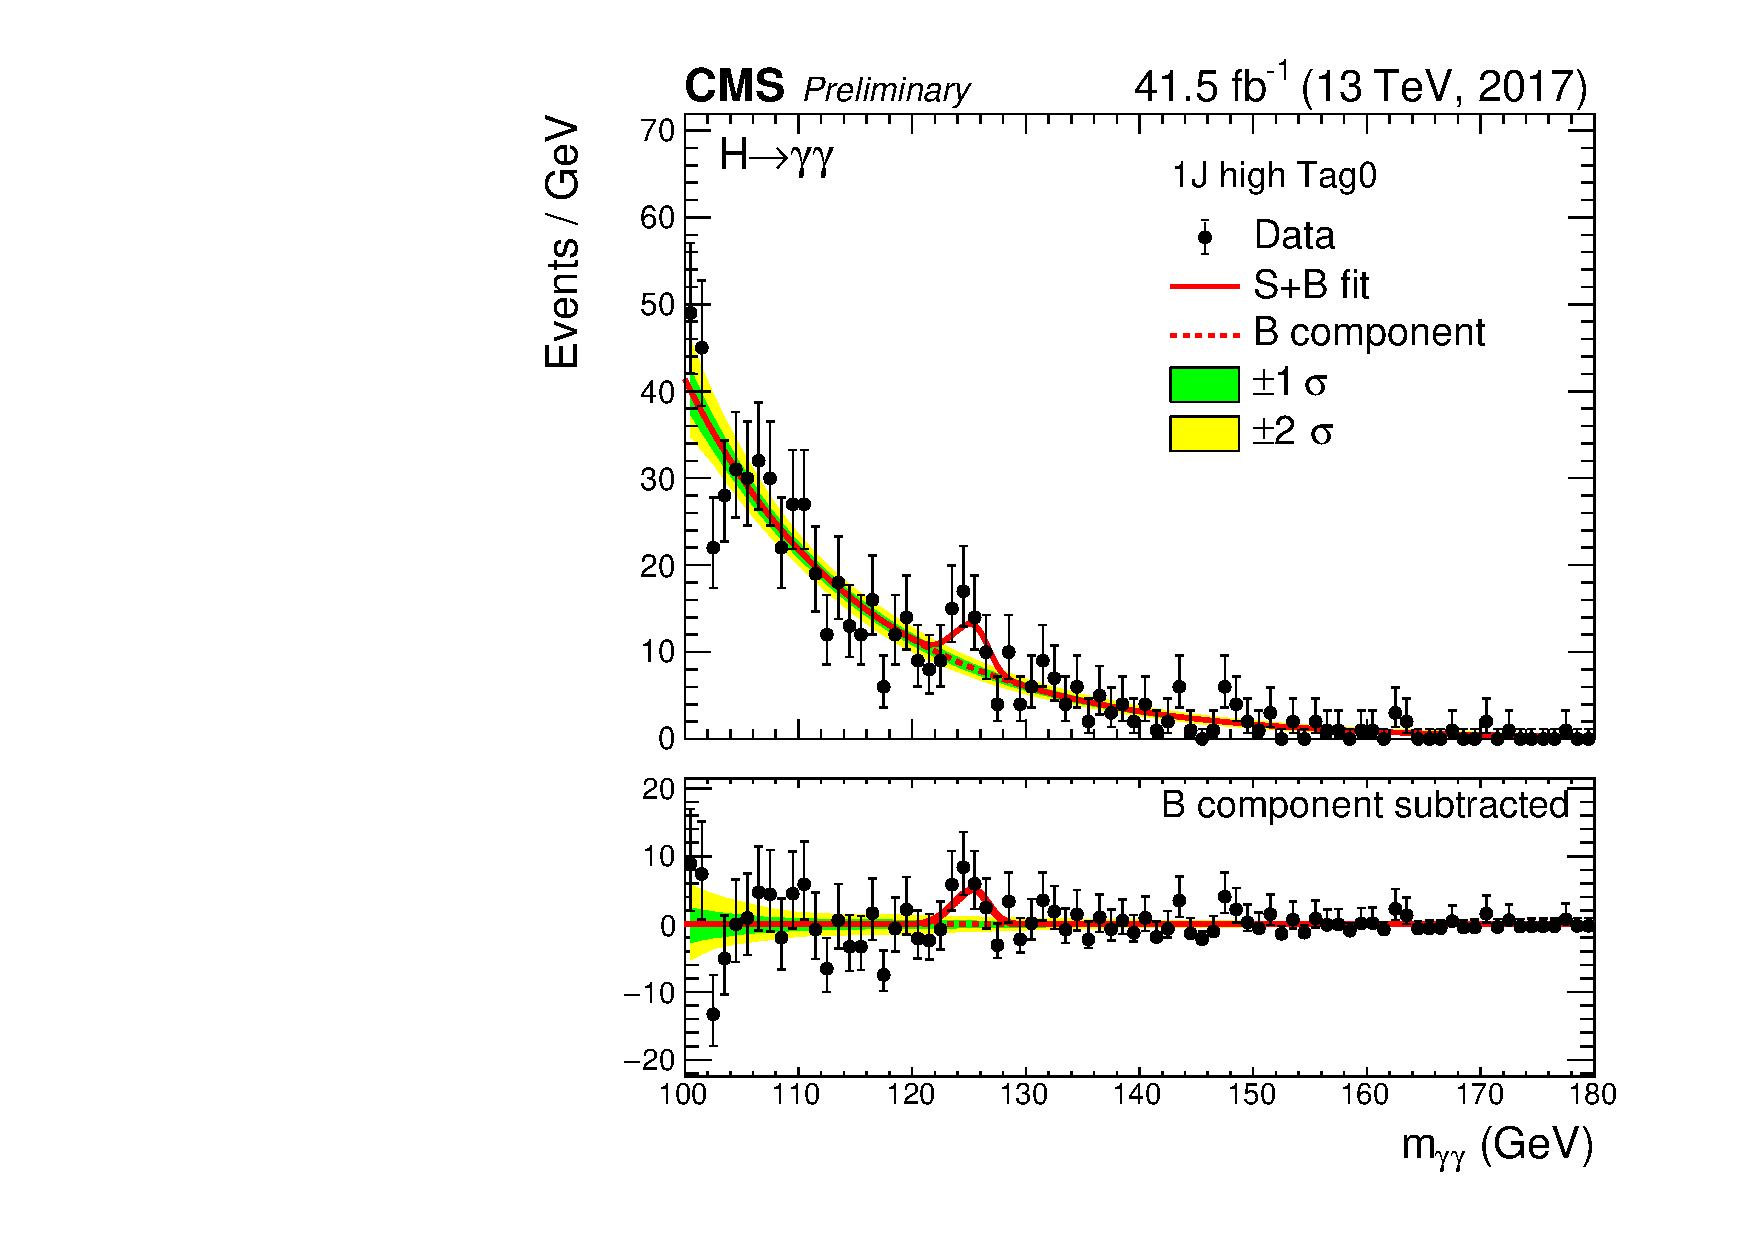
\includegraphics[width=0.49\textwidth]{Figures/Appendices/_forAppendix2017ch2_RECO_1J_PTH_120_200_Tag0_13TeV.pdf}
  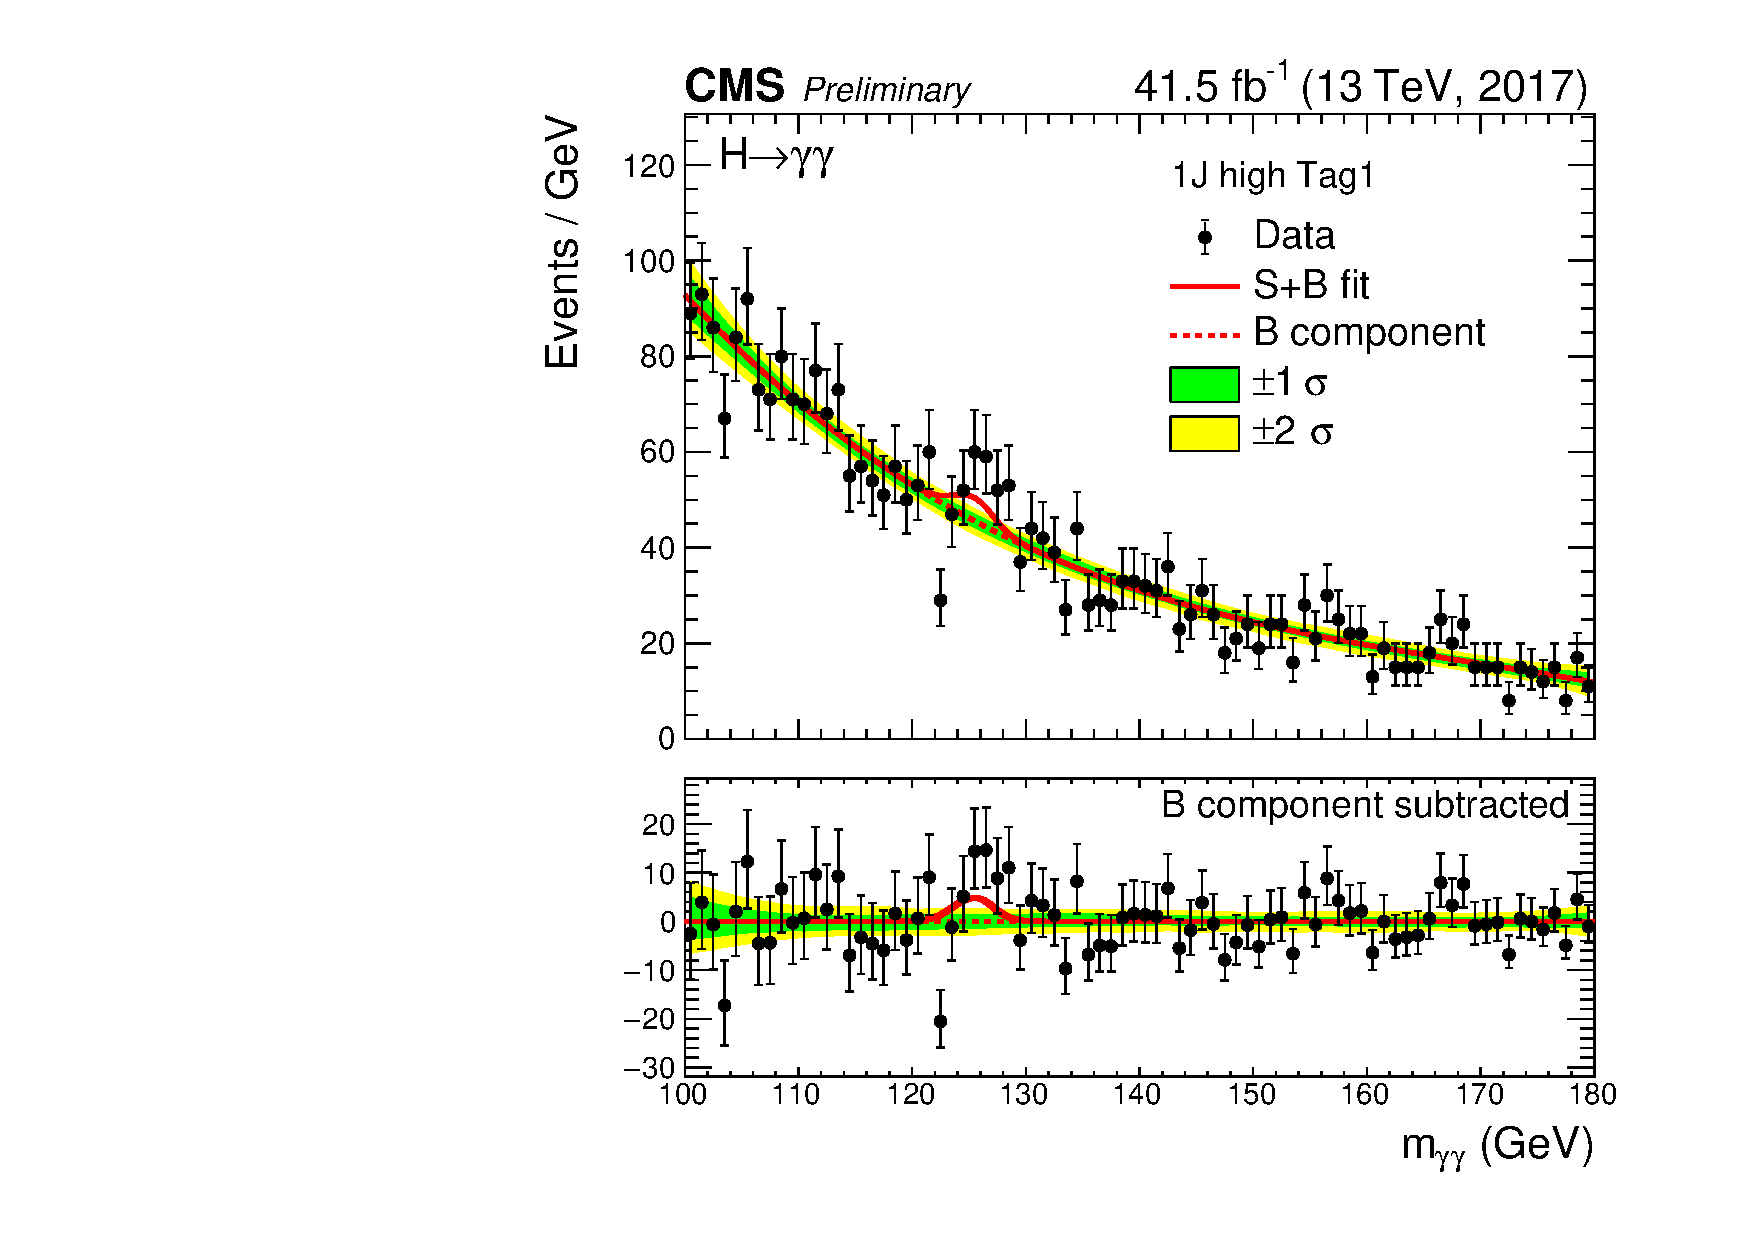
\includegraphics[width=0.49\textwidth]{Figures/Appendices/_forAppendix2017ch2_RECO_1J_PTH_120_200_Tag1_13TeV.pdf}
  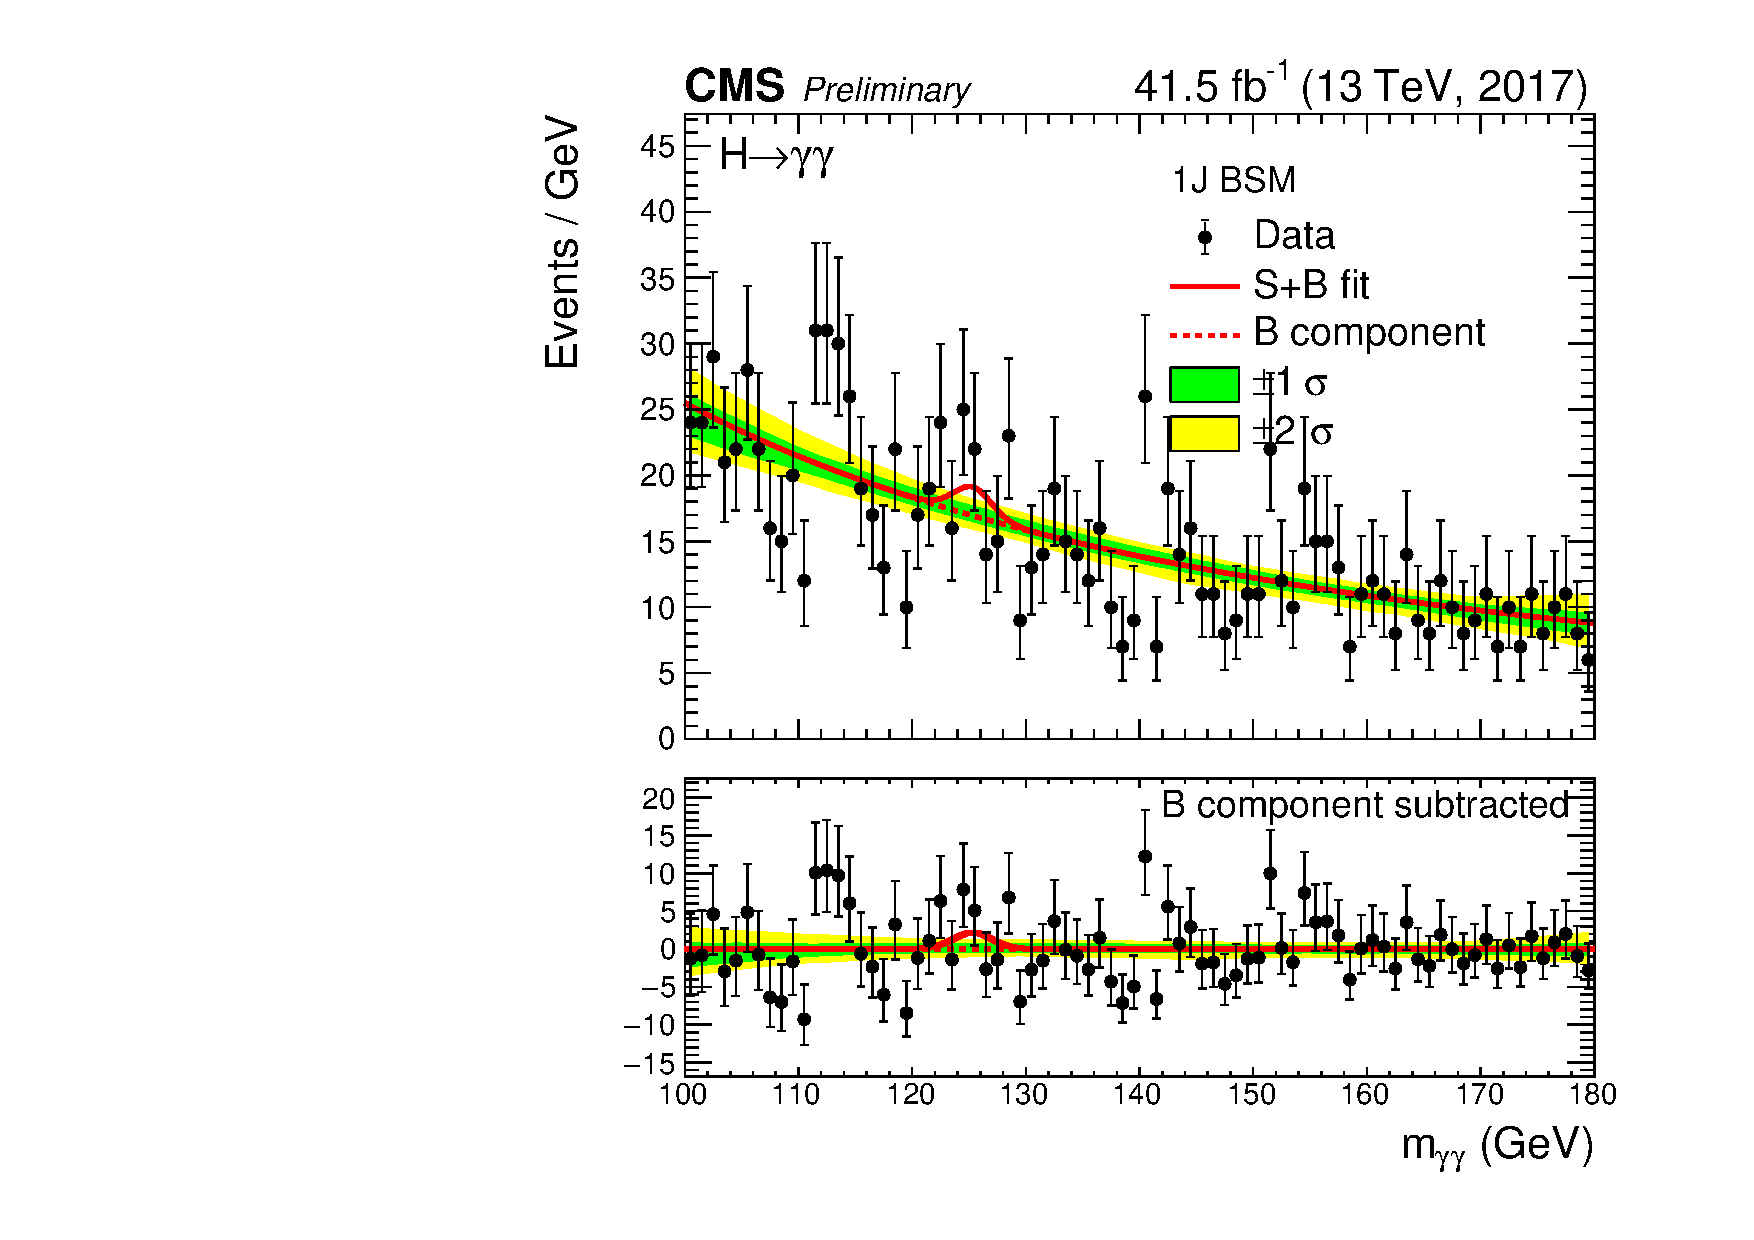
\includegraphics[width=0.49\textwidth]{Figures/Appendices/_forAppendix2017ch2_RECO_1J_PTH_GT200_13TeV.pdf}
  \caption[Signal plus background fits to data.]
  {
    Data points (black) and signal plus background model fit are shown. 
    The one standard deviation (green) and two standard deviation (yellow) bands 
    include the uncertainties in the background component of the fit. 
    The solid red line shows the contribution from the total signal, plus the background contribution. 
    The dashed red line shows the contribution from the background component of the fit. 
    The bottom plot shows the residuals after subtraction of this background component.
  }
\end{figure}

\begin{figure}[hptb]
  \centering
  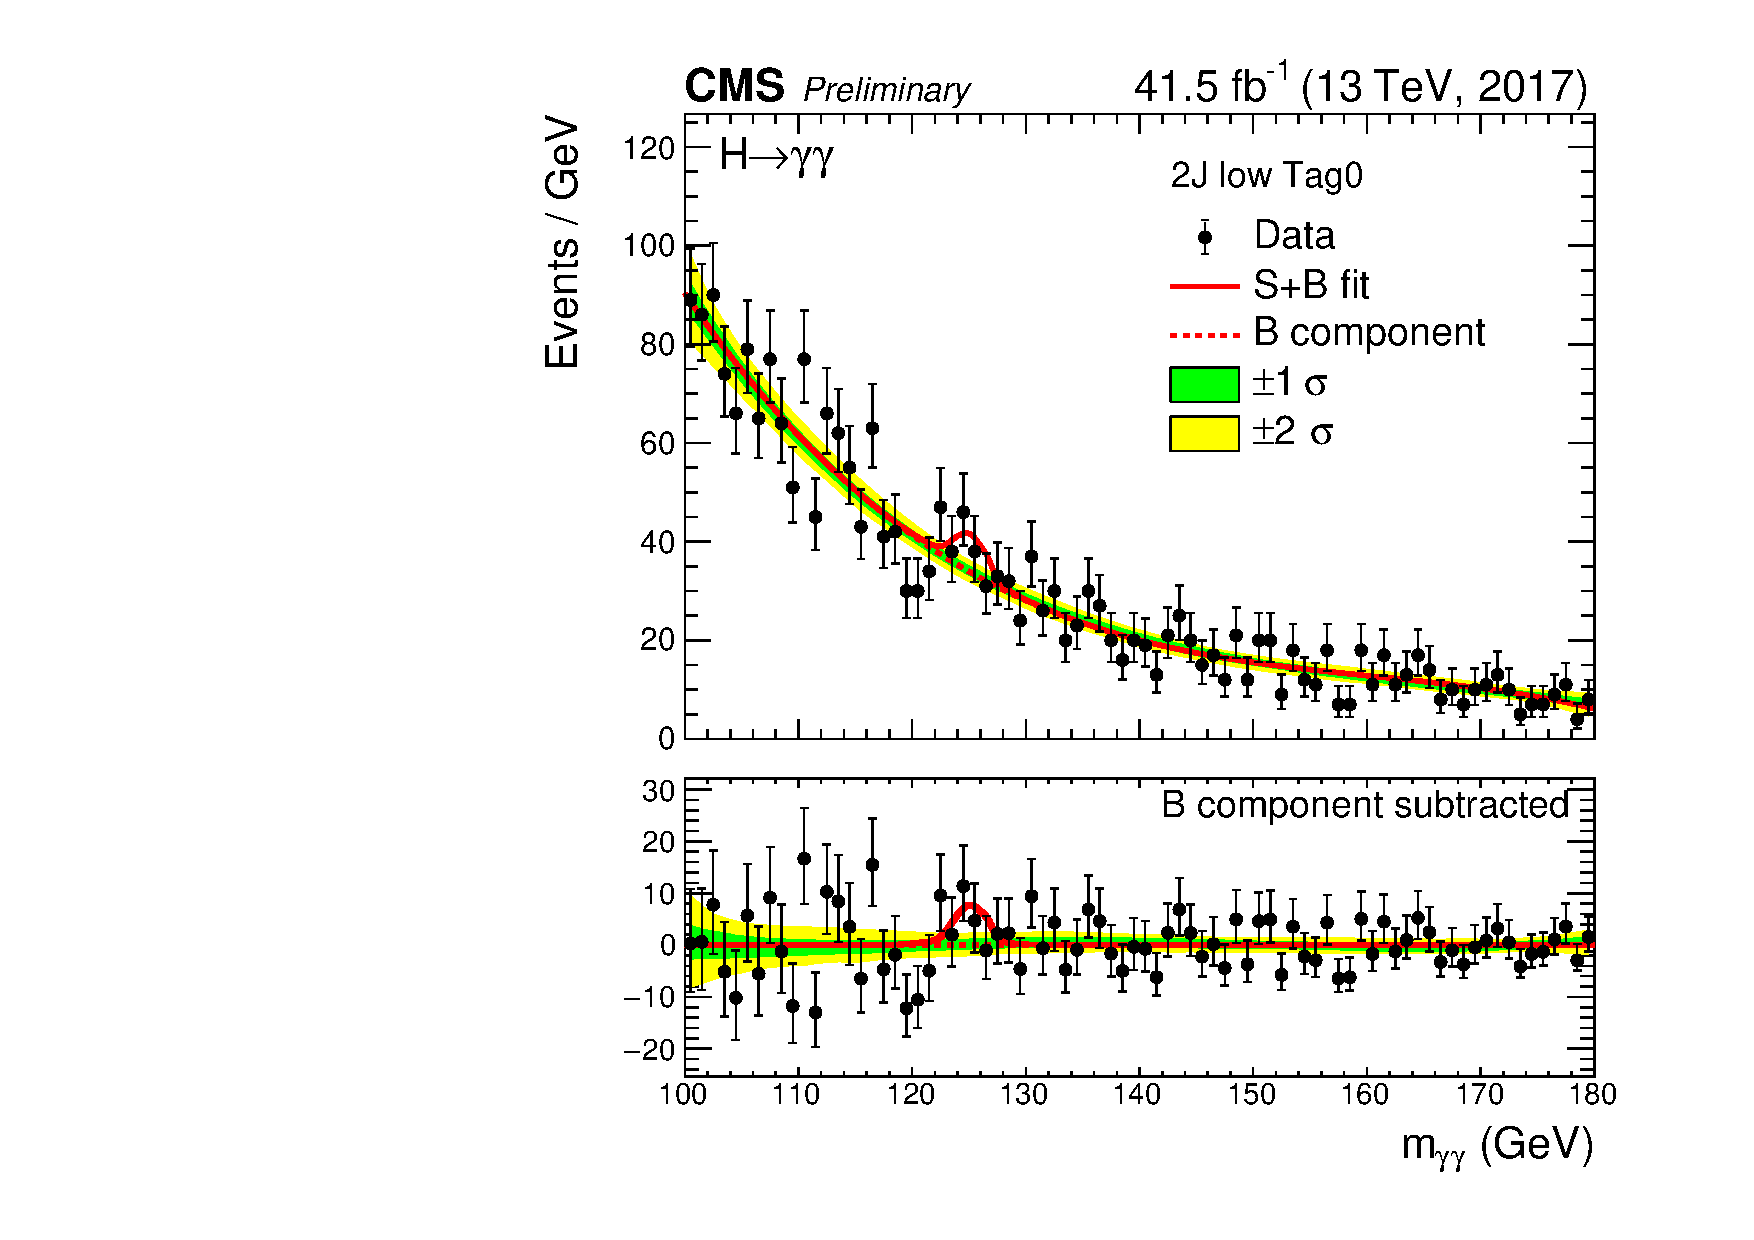
\includegraphics[width=0.49\textwidth]{Figures/Appendices/_forAppendix2017ch2_RECO_GE2J_PTH_0_60_Tag0_13TeV.pdf}
  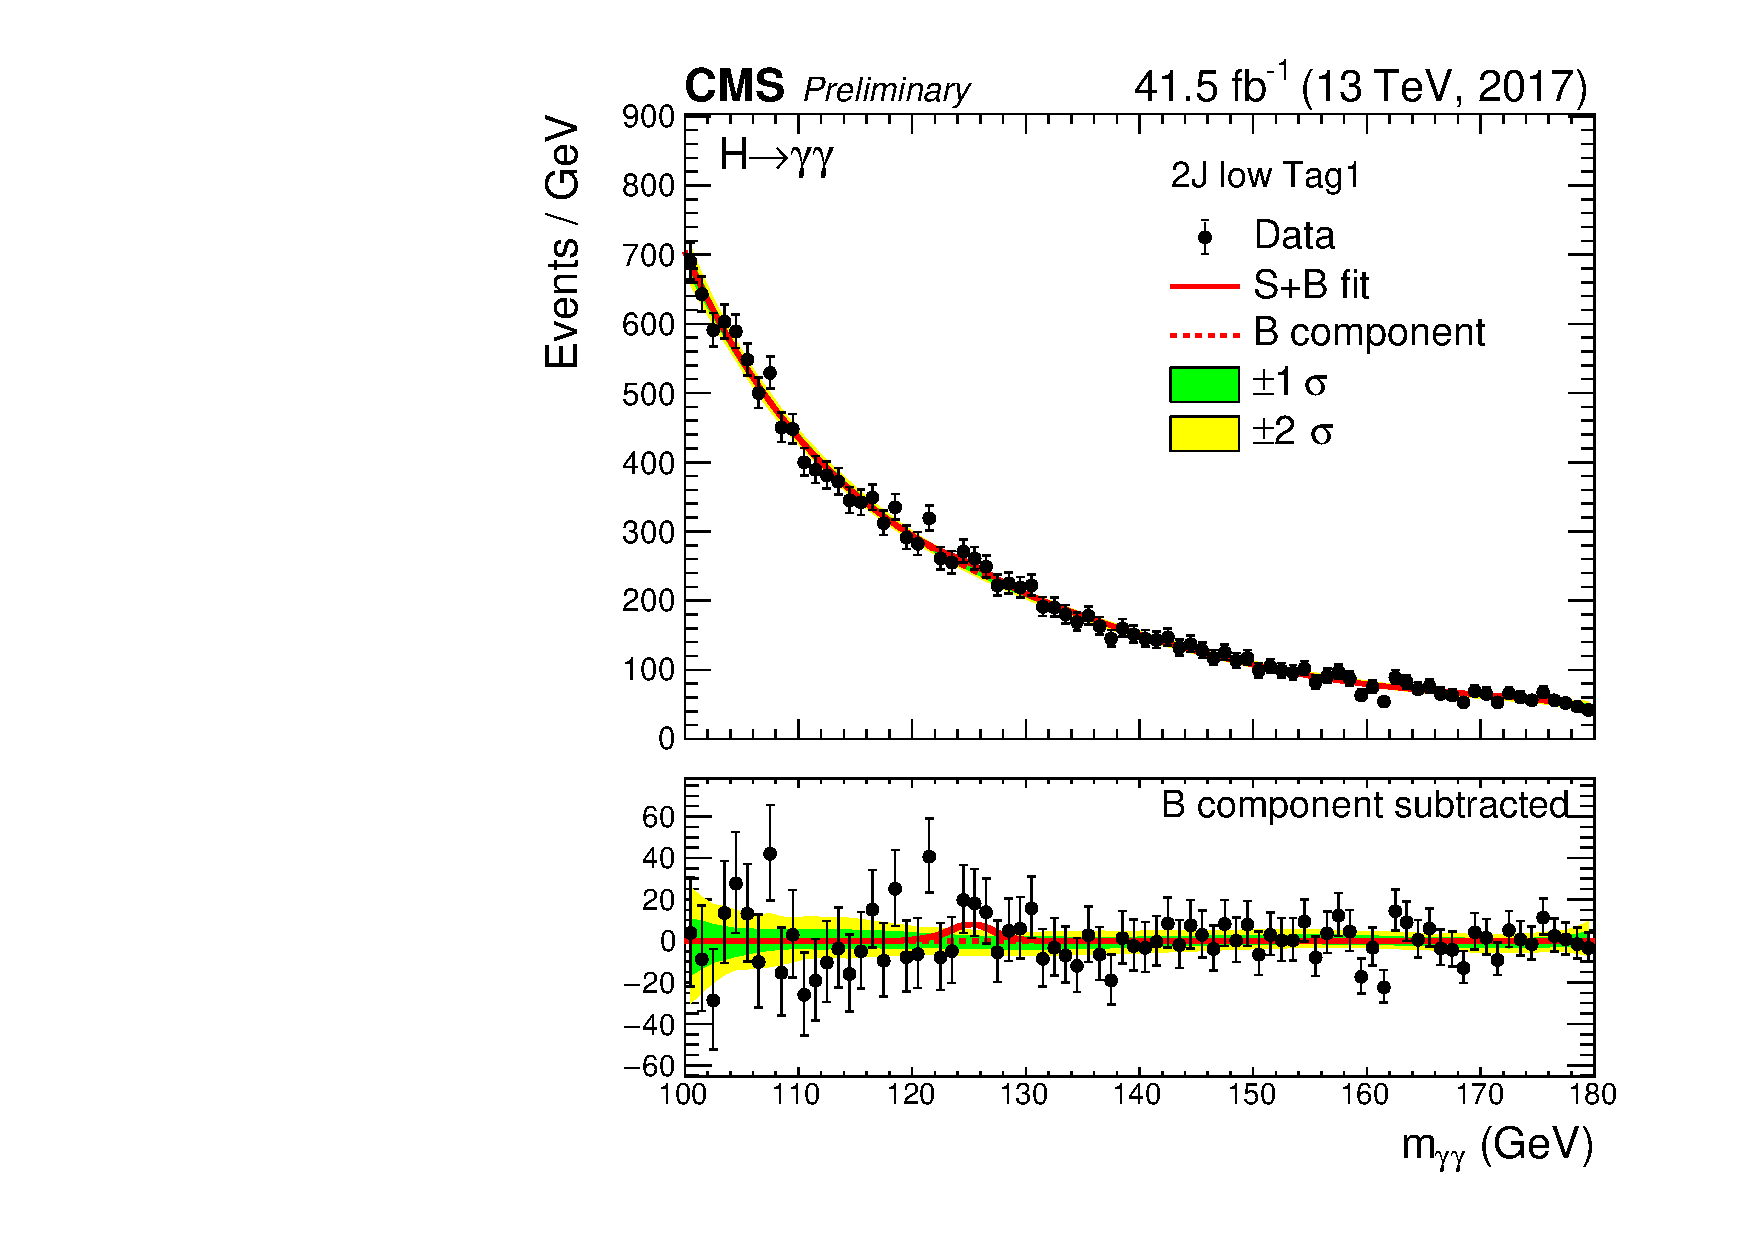
\includegraphics[width=0.49\textwidth]{Figures/Appendices/_forAppendix2017ch2_RECO_GE2J_PTH_0_60_Tag1_13TeV.pdf}
  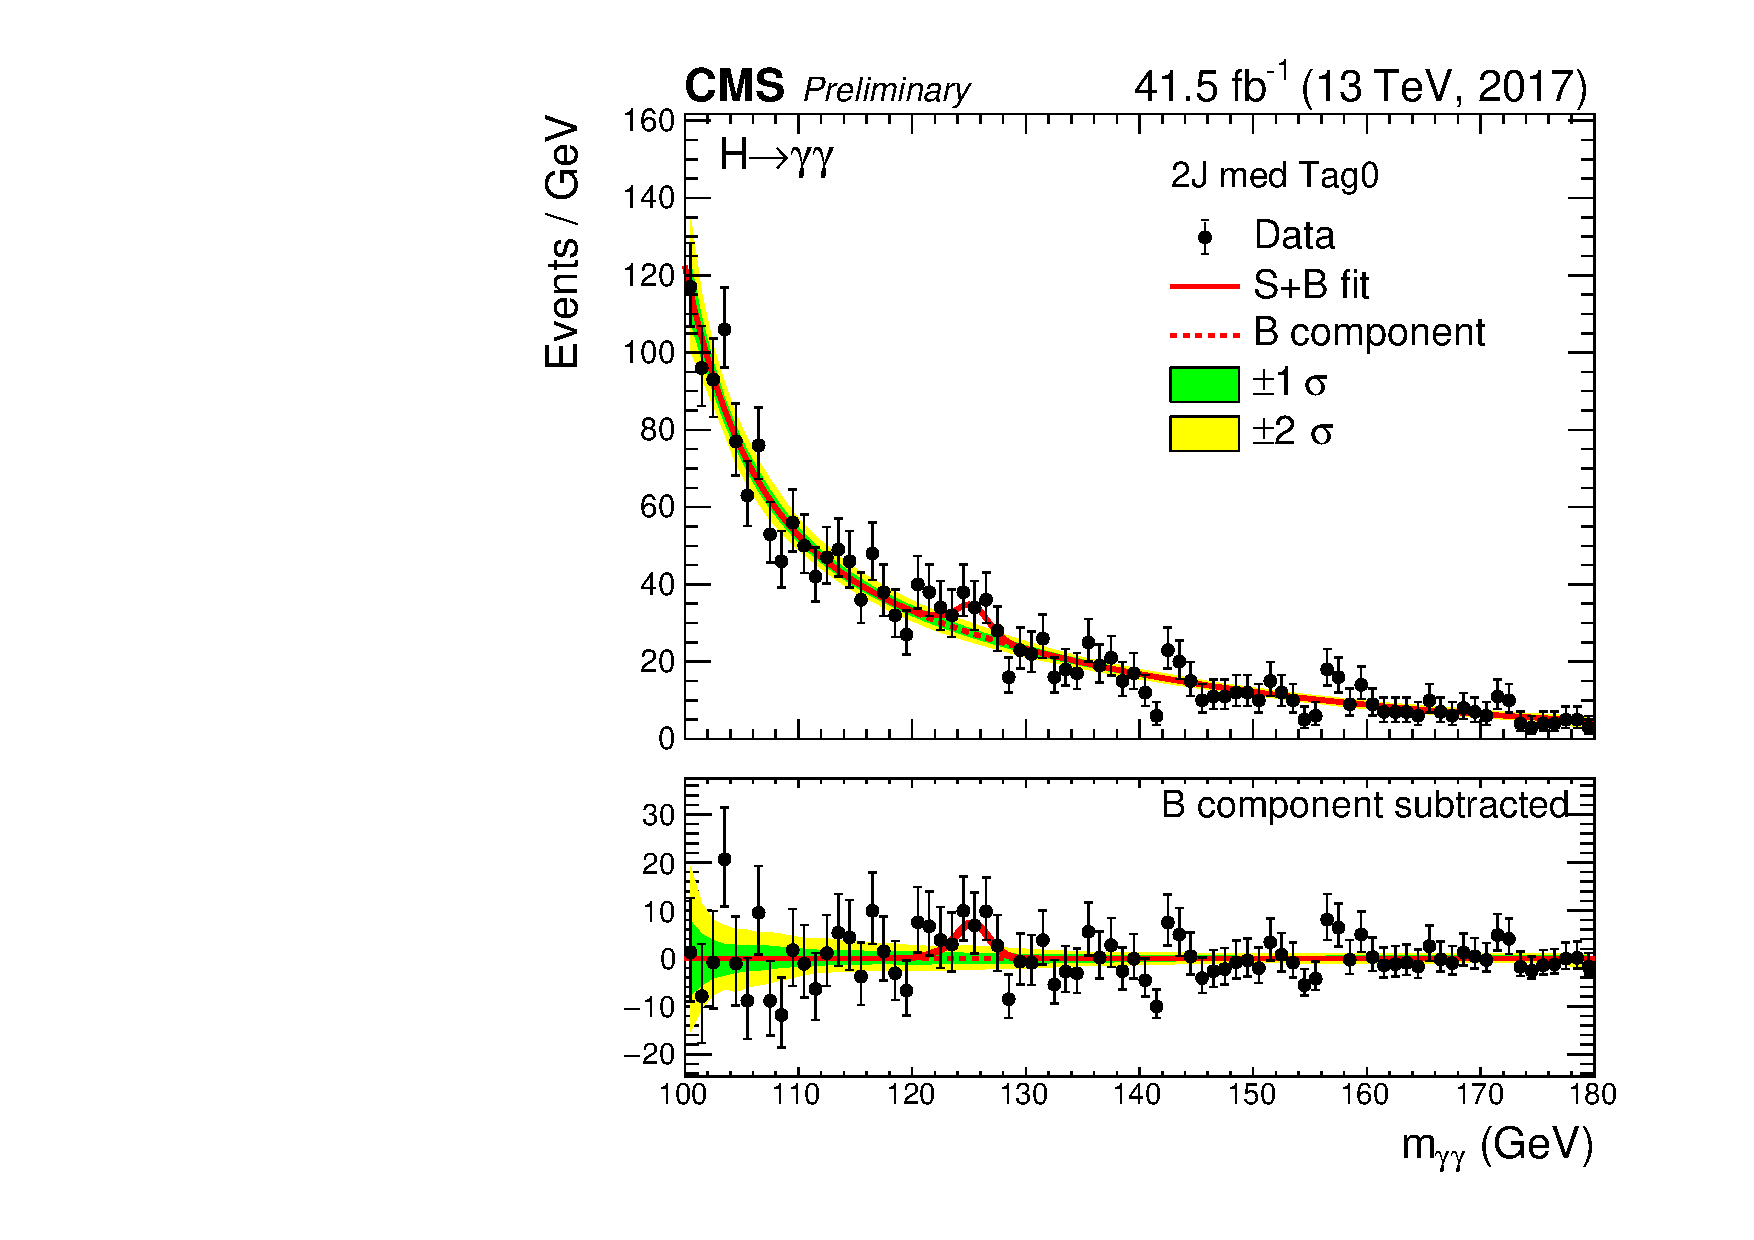
\includegraphics[width=0.49\textwidth]{Figures/Appendices/_forAppendix2017ch2_RECO_GE2J_PTH_60_120_Tag0_13TeV.pdf}
  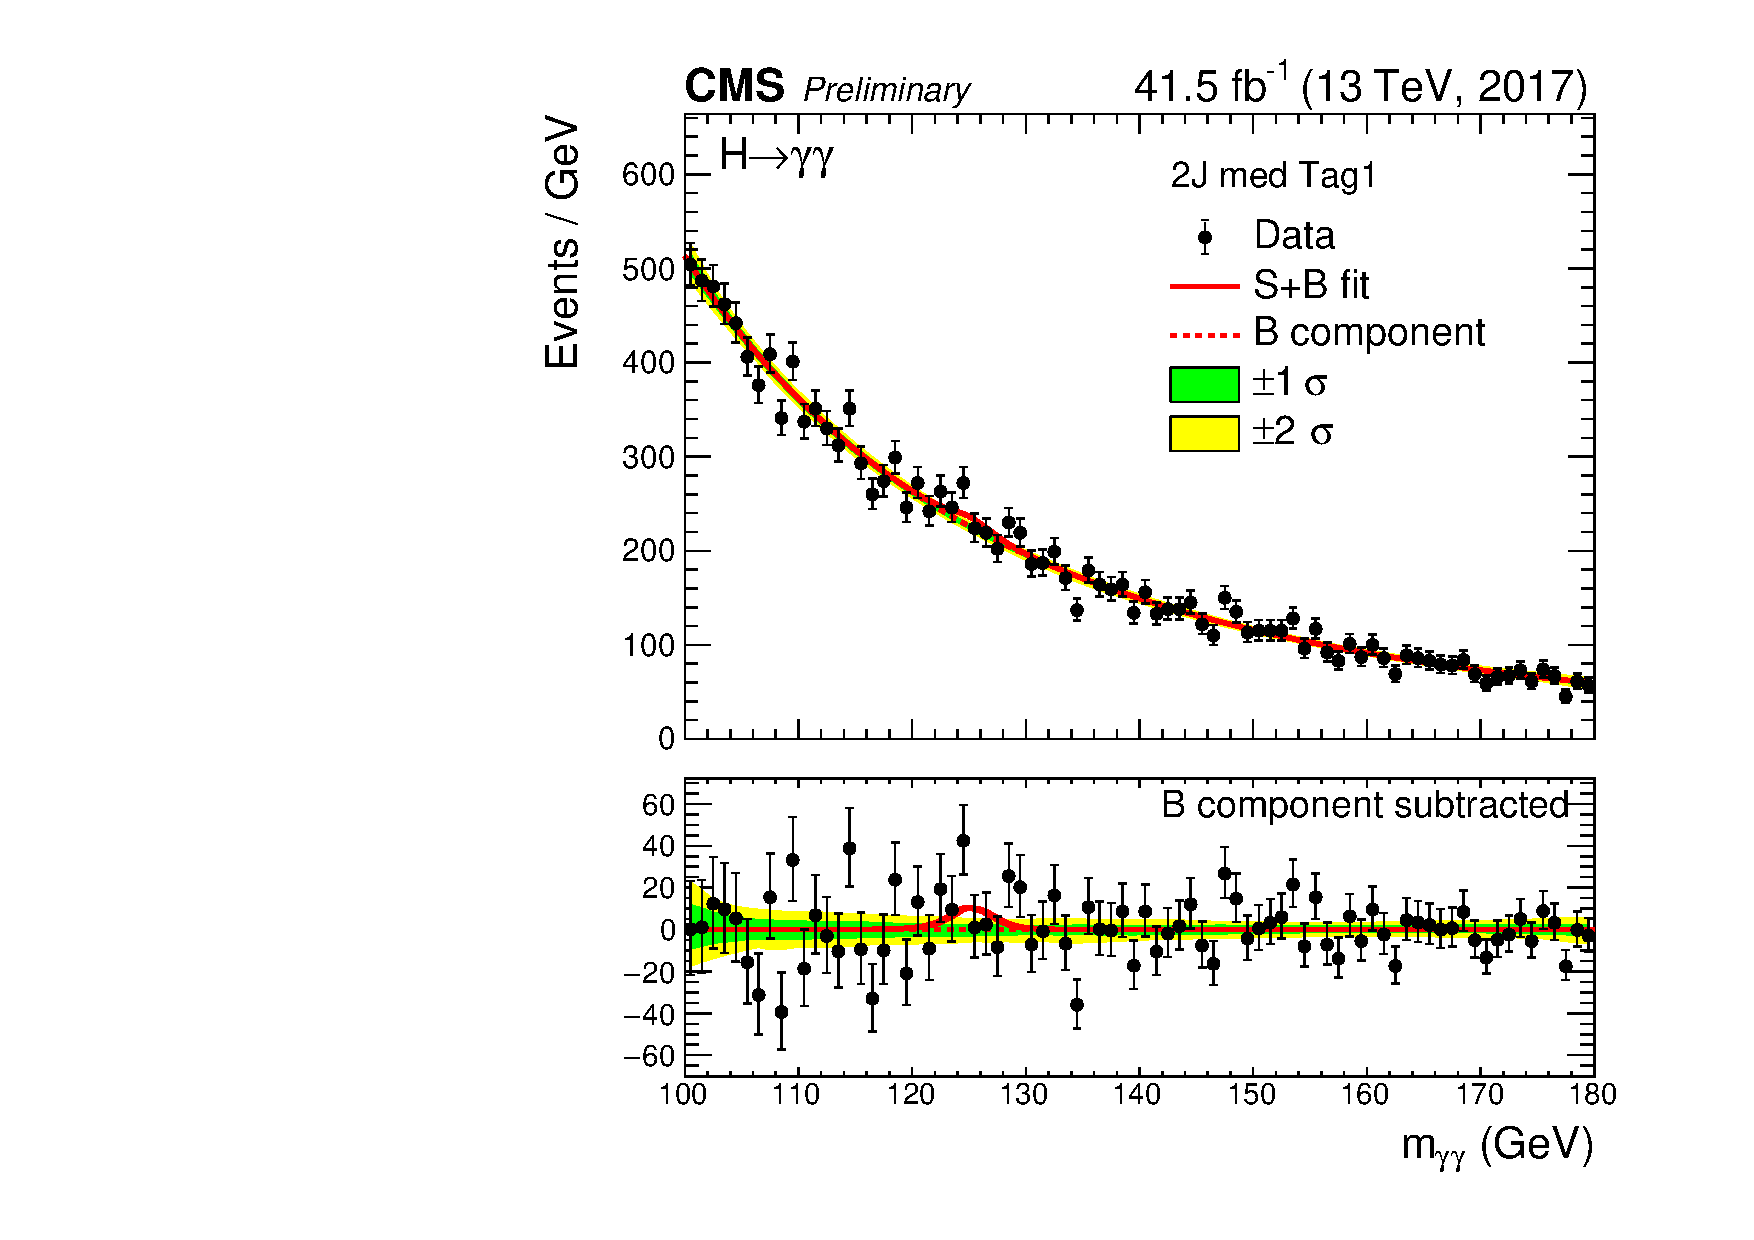
\includegraphics[width=0.49\textwidth]{Figures/Appendices/_forAppendix2017ch2_RECO_GE2J_PTH_60_120_Tag1_13TeV.pdf}
  \caption[Signal plus background fits to data.]
  {
    Data points (black) and signal plus background model fit are shown. 
    The one standard deviation (green) and two standard deviation (yellow) bands 
    include the uncertainties in the background component of the fit. 
    The solid red line shows the contribution from the total signal, plus the background contribution. 
    The dashed red line shows the contribution from the background component of the fit. 
    The bottom plot shows the residuals after subtraction of this background component.
  }
\end{figure}

\begin{figure}[hptb]
  \centering
  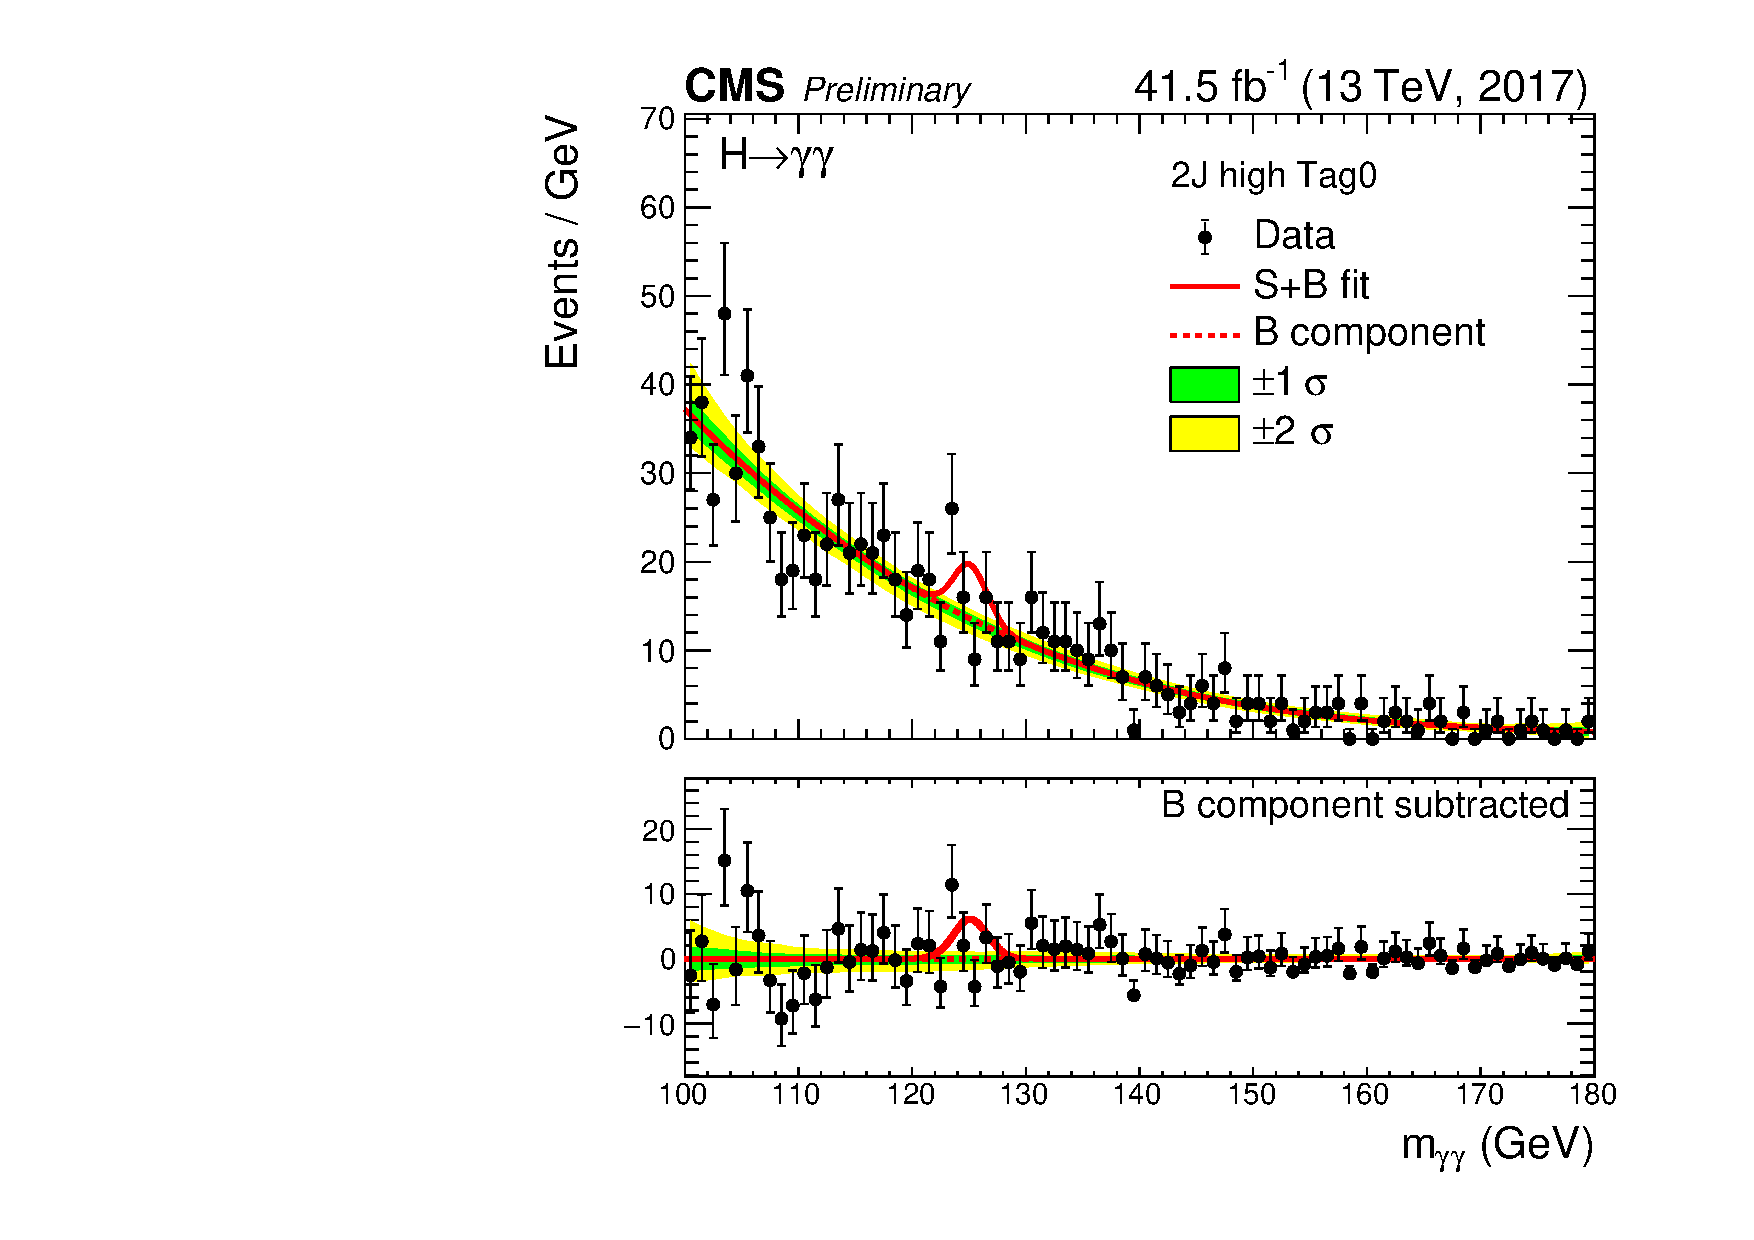
\includegraphics[width=0.49\textwidth]{Figures/Appendices/_forAppendix2017ch2_RECO_GE2J_PTH_120_200_Tag0_13TeV.pdf}
  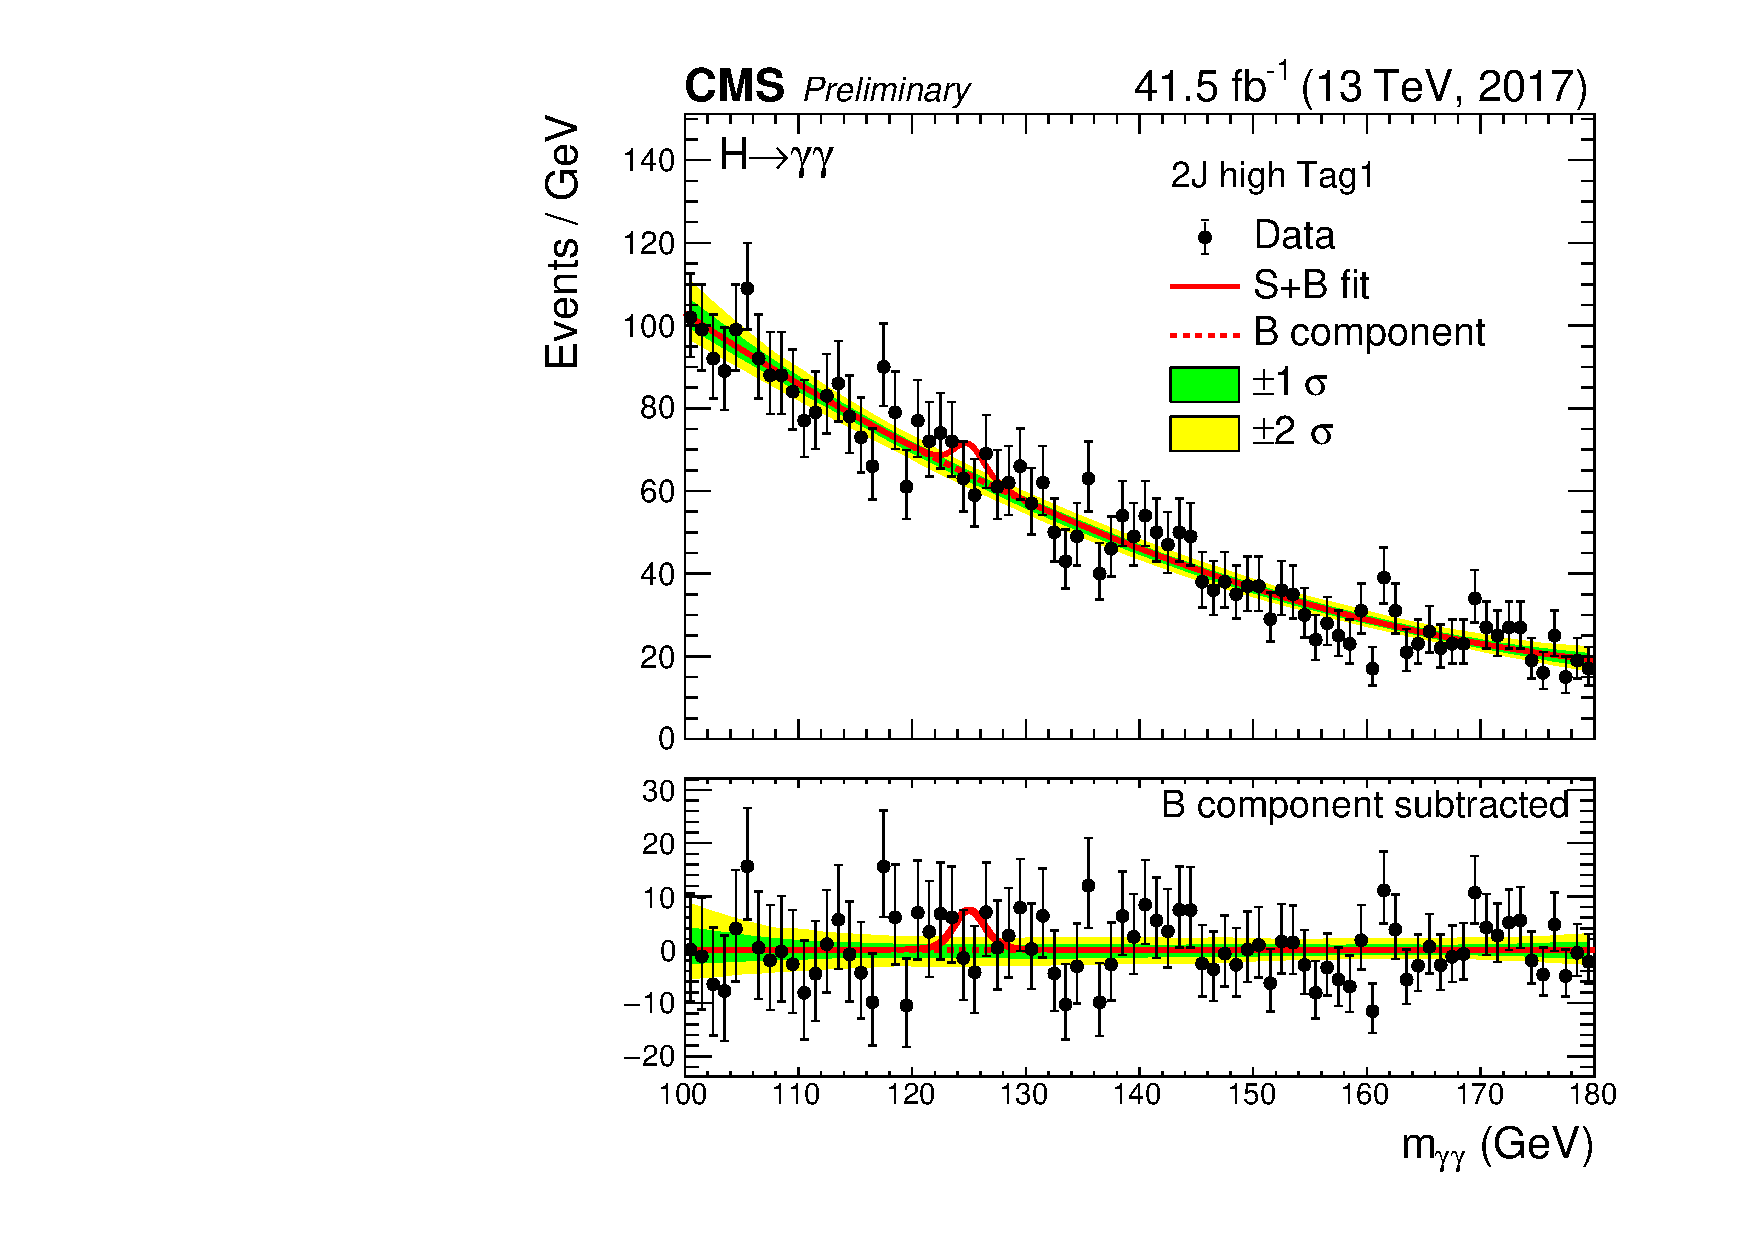
\includegraphics[width=0.49\textwidth]{Figures/Appendices/_forAppendix2017ch2_RECO_GE2J_PTH_120_200_Tag1_13TeV.pdf}
  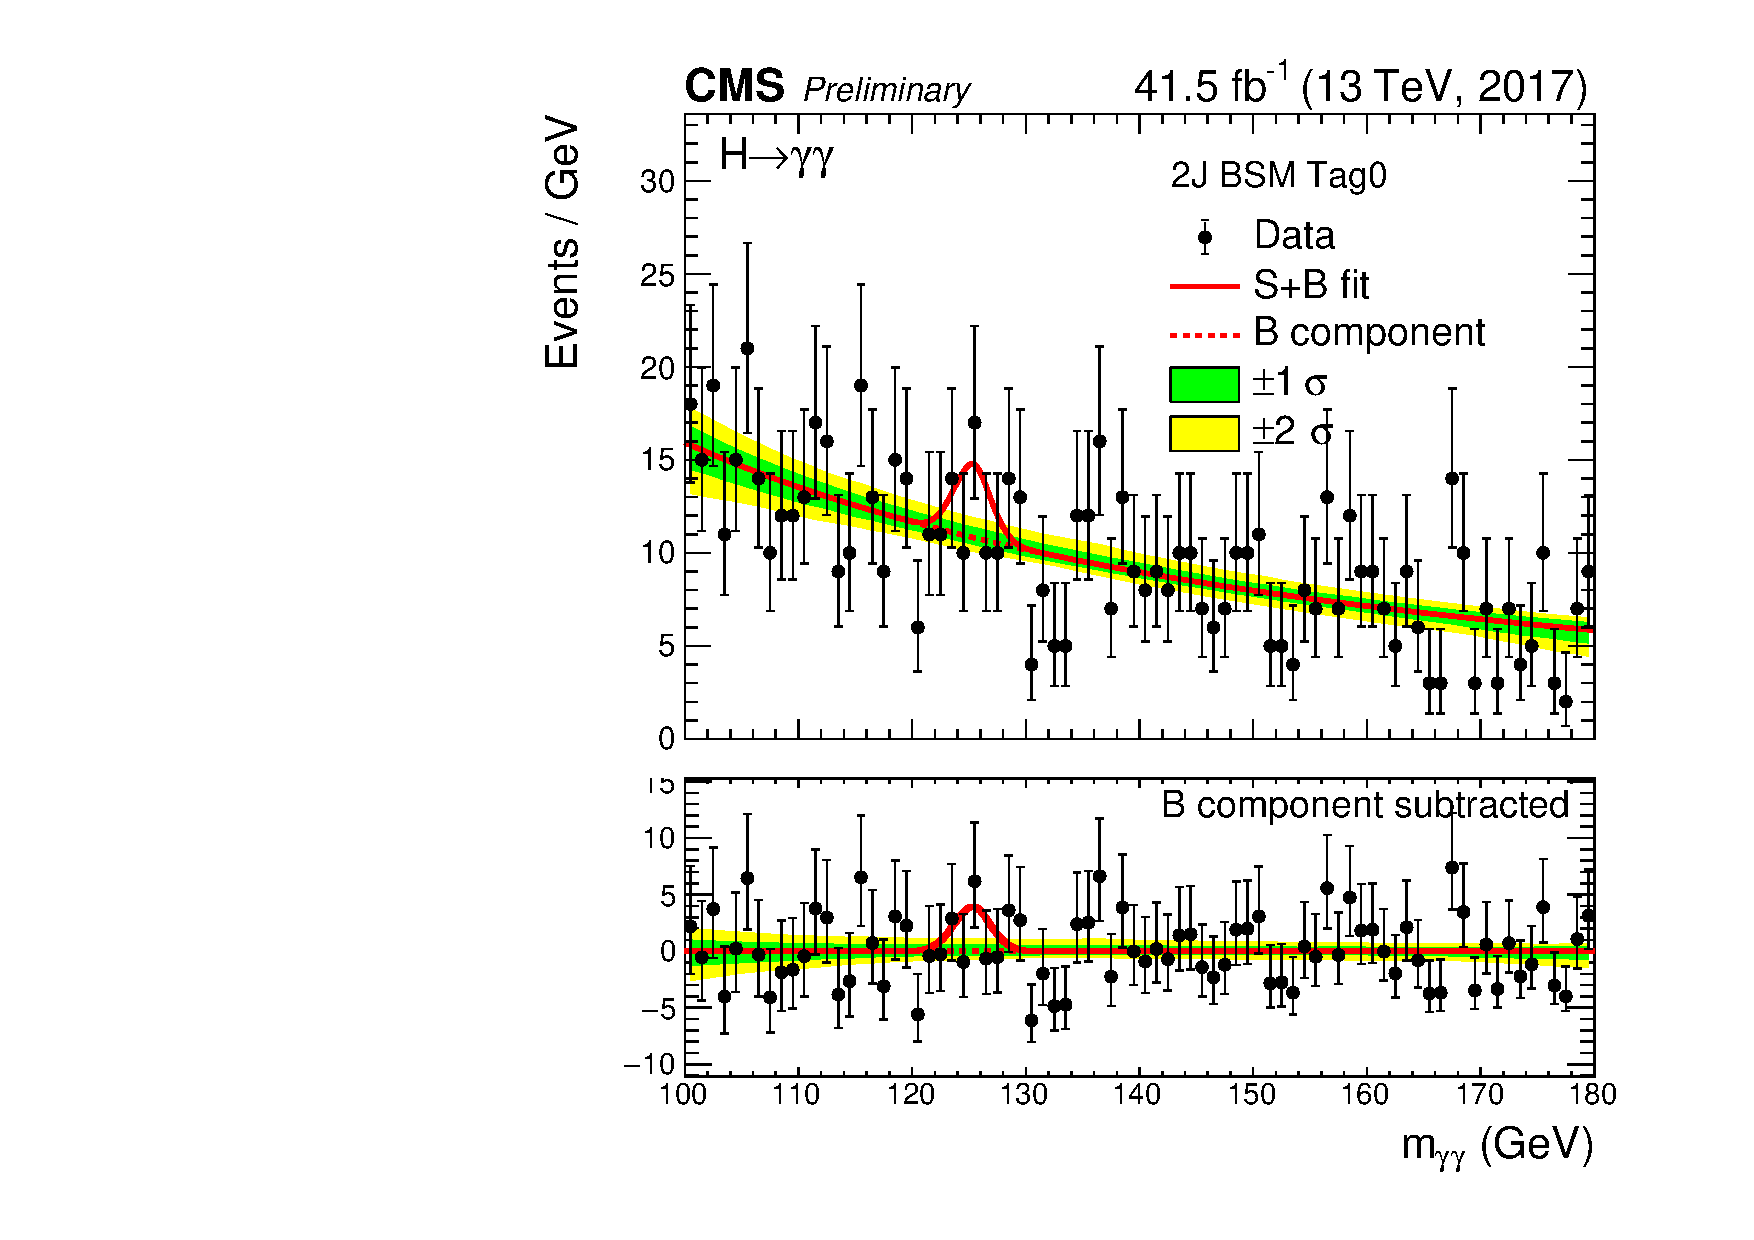
\includegraphics[width=0.49\textwidth]{Figures/Appendices/_forAppendix2017ch2_RECO_GE2J_PTH_GT200_Tag0_13TeV.pdf}
  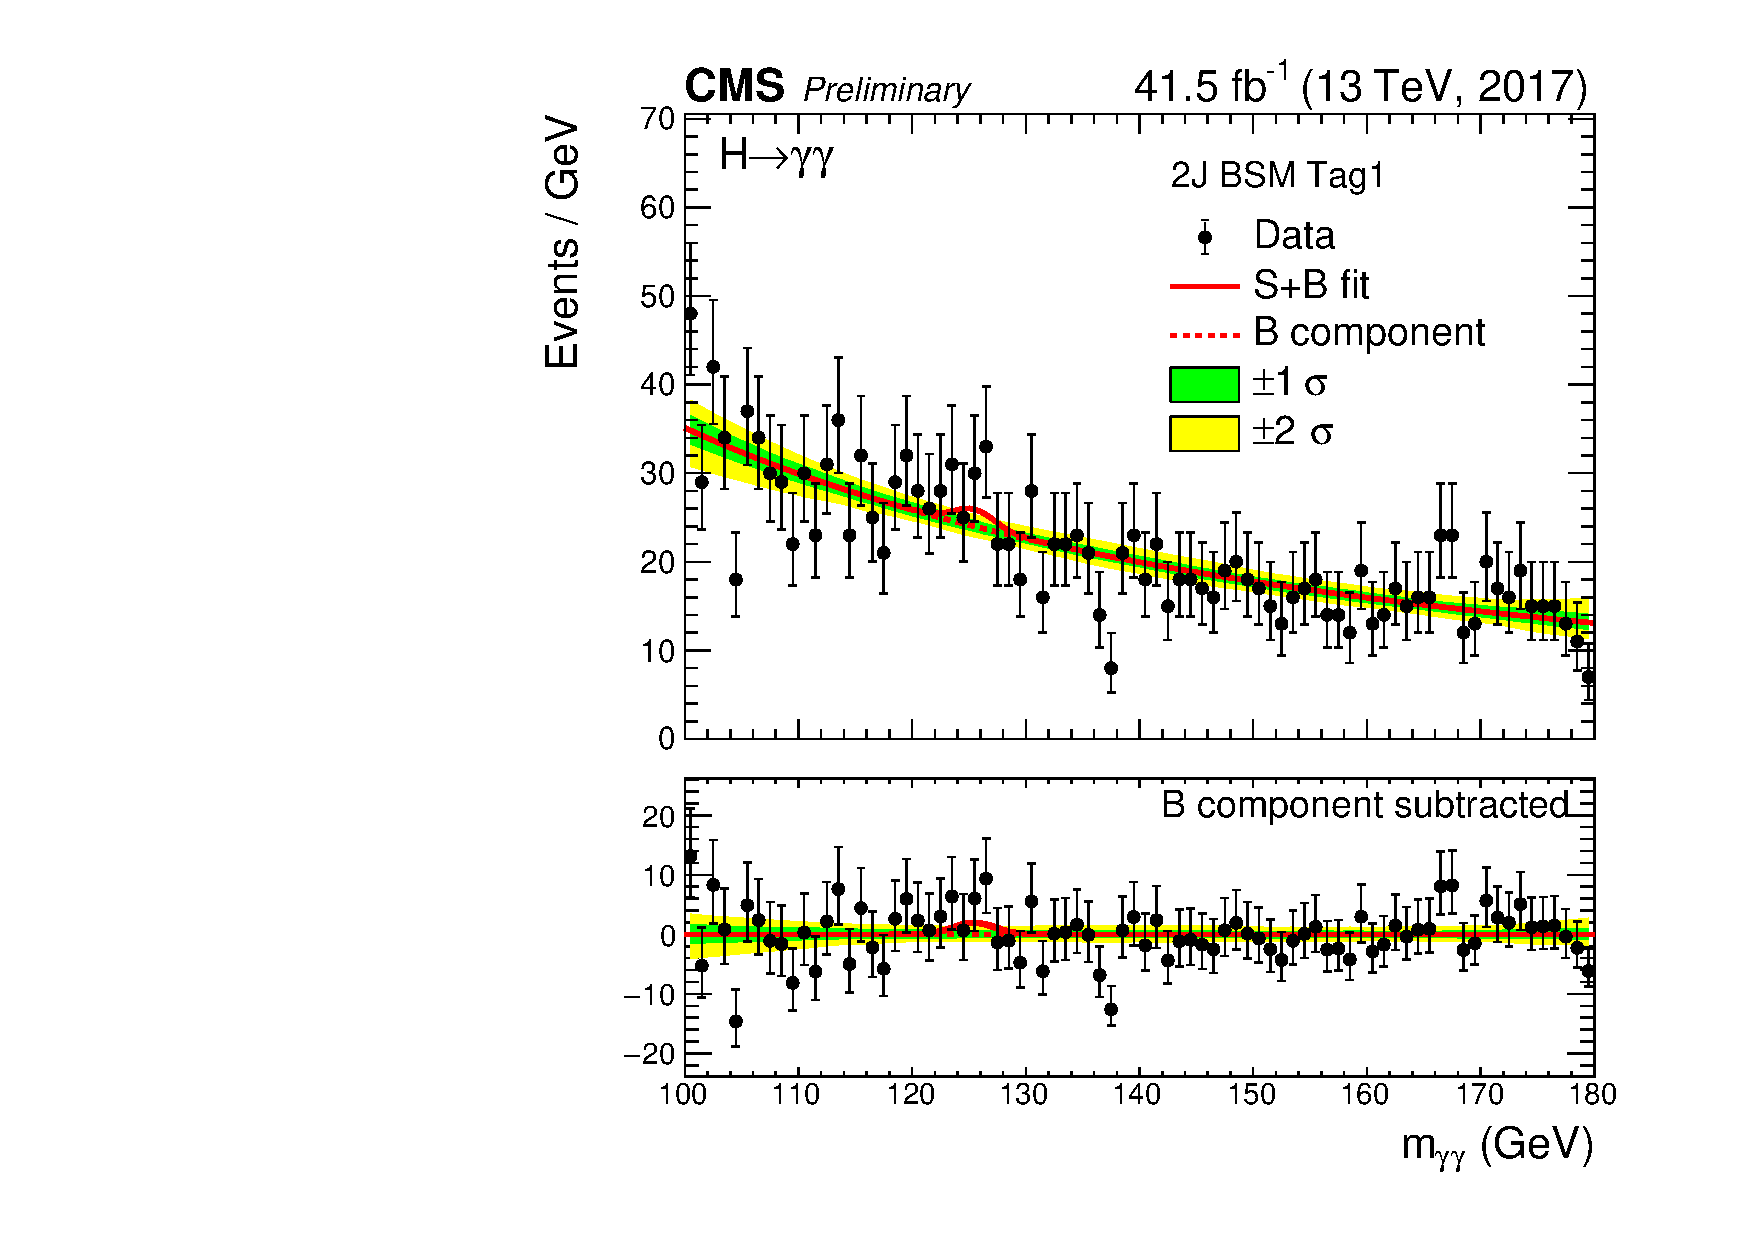
\includegraphics[width=0.49\textwidth]{Figures/Appendices/_forAppendix2017ch2_RECO_GE2J_PTH_GT200_Tag1_13TeV.pdf}
  \caption[Signal plus background fits to data.]
  {
    Data points (black) and signal plus background model fit are shown. 
    The one standard deviation (green) and two standard deviation (yellow) bands 
    include the uncertainties in the background component of the fit. 
    The solid red line shows the contribution from the total signal, plus the background contribution. 
    The dashed red line shows the contribution from the background component of the fit. 
    The bottom plot shows the residuals after subtraction of this background component.
  }
\end{figure}

\begin{figure}[hptb]
  \centering
  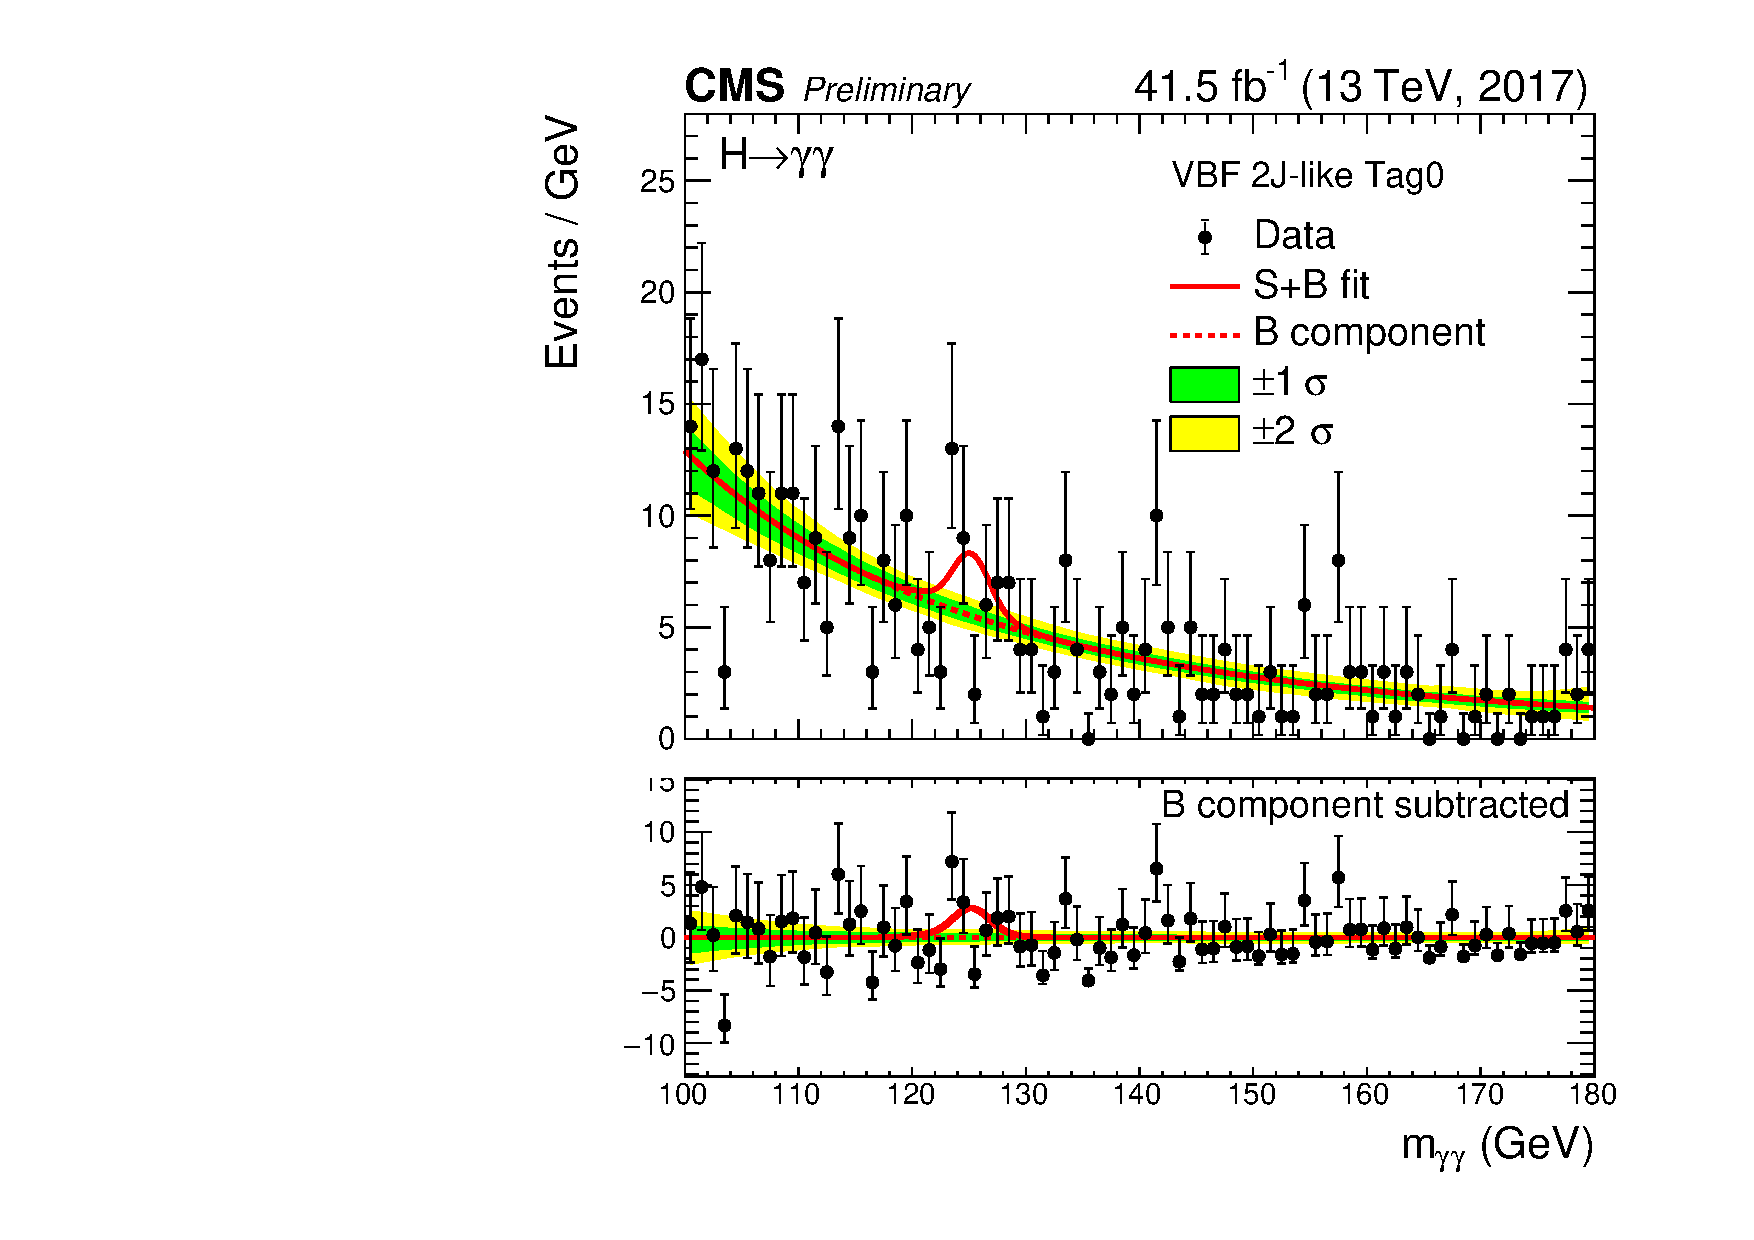
\includegraphics[width=0.49\textwidth]{Figures/Appendices/_forAppendix2017ch2_RECO_VBFTOPO_JET3VETO_Tag0_13TeV.pdf}
  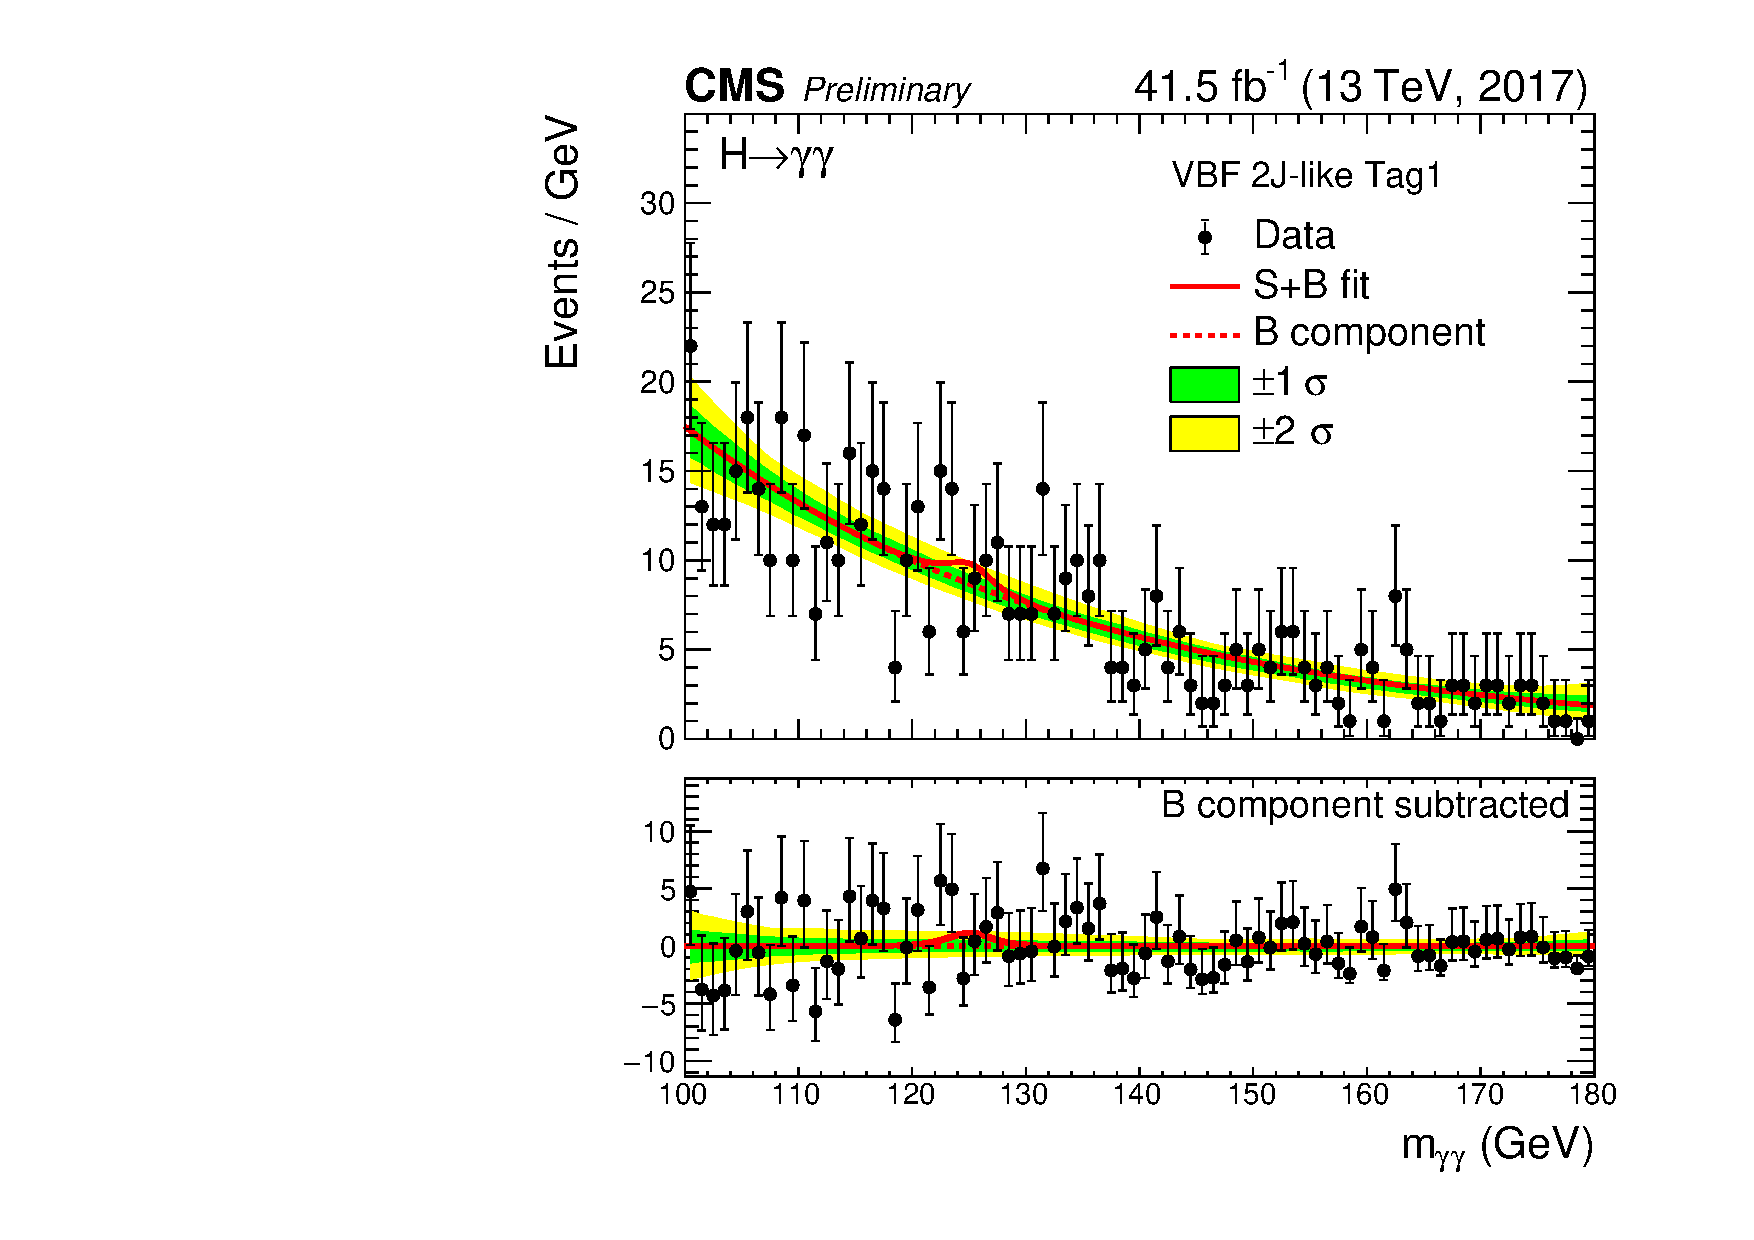
\includegraphics[width=0.49\textwidth]{Figures/Appendices/_forAppendix2017ch2_RECO_VBFTOPO_JET3VETO_Tag1_13TeV.pdf}
  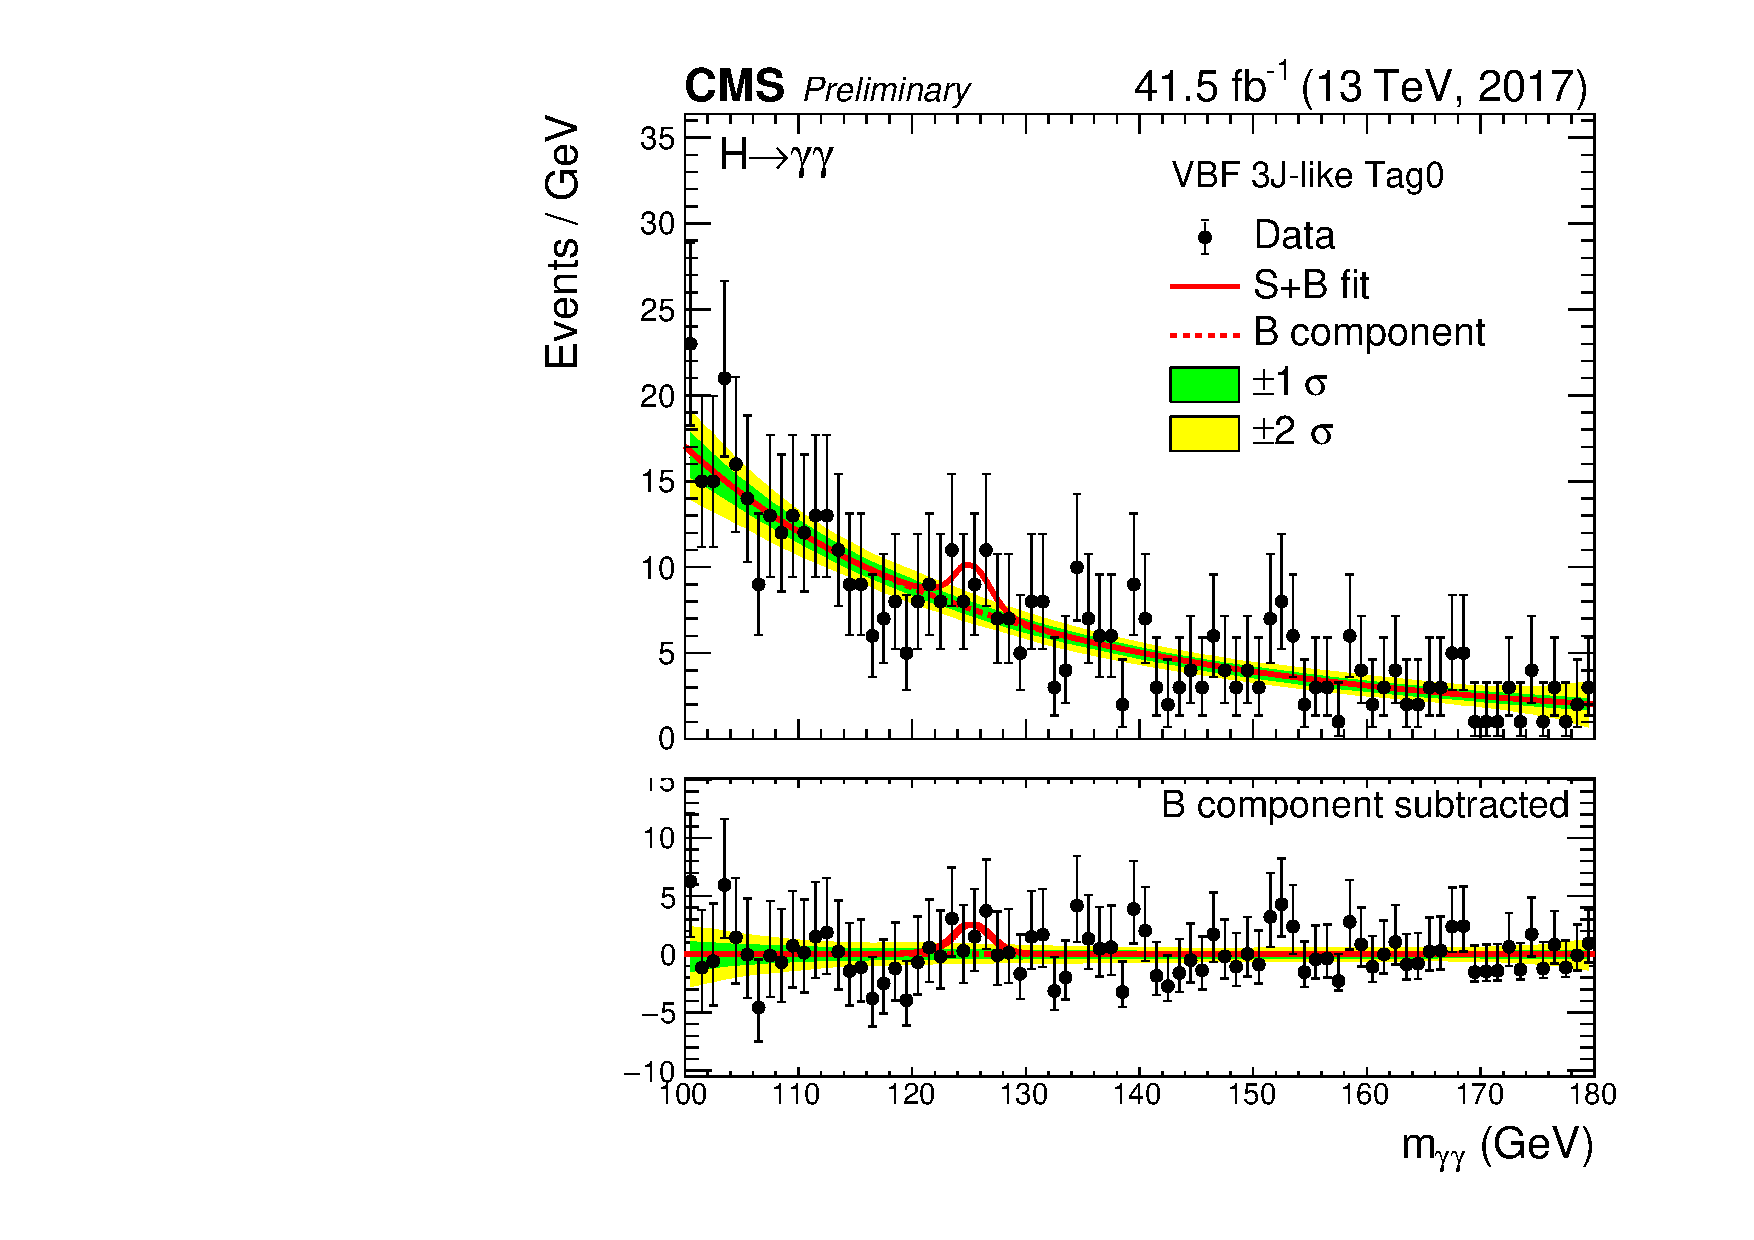
\includegraphics[width=0.49\textwidth]{Figures/Appendices/_forAppendix2017ch2_RECO_VBFTOPO_JET3_Tag0_13TeV.pdf}
  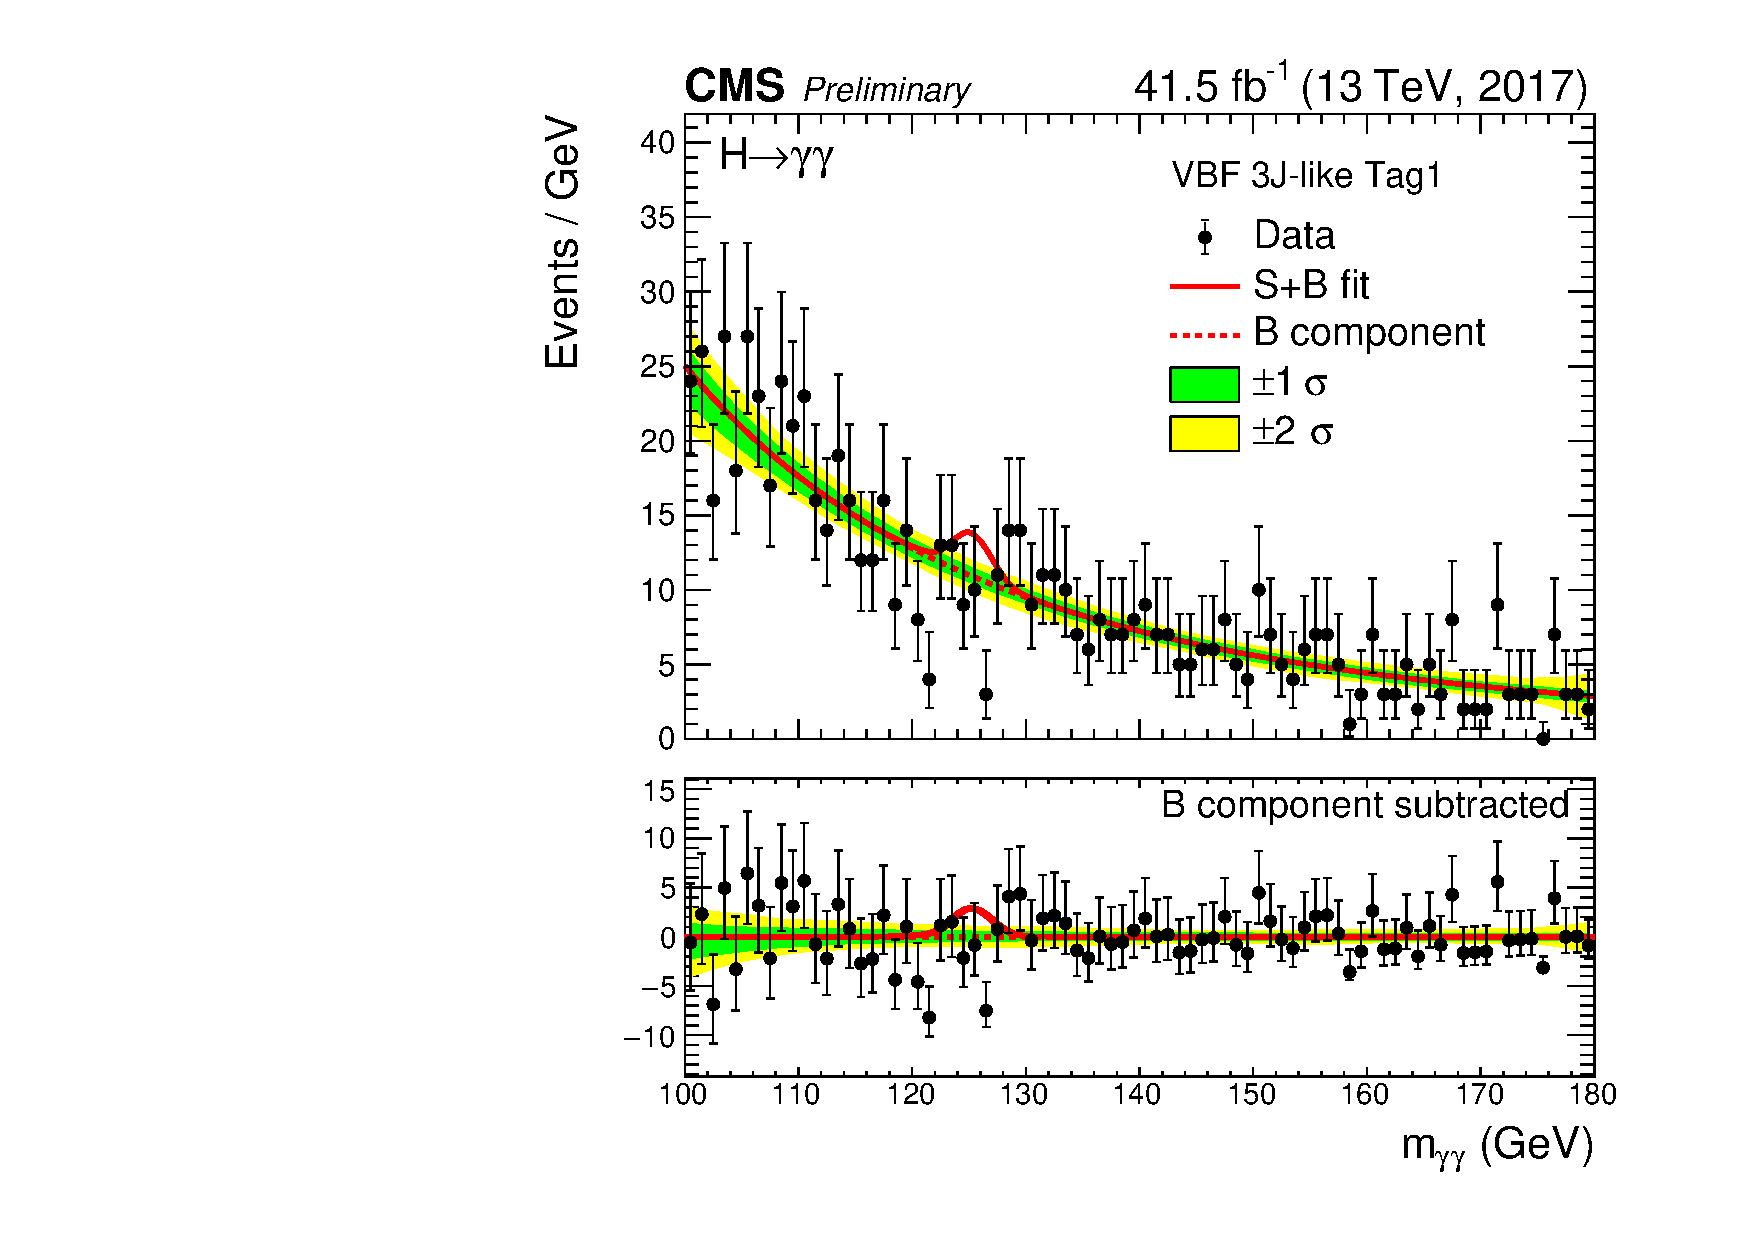
\includegraphics[width=0.49\textwidth]{Figures/Appendices/_forAppendix2017ch2_RECO_VBFTOPO_JET3_Tag1_13TeV.pdf}
  \caption[Signal plus background fits to data.]
  {
    Data points (black) and signal plus background model fit are shown. 
    The one standard deviation (green) and two standard deviation (yellow) bands 
    include the uncertainties in the background component of the fit. 
    The solid red line shows the contribution from the total signal, plus the background contribution. 
    The dashed red line shows the contribution from the background component of the fit. 
    The bottom plot shows the residuals after subtraction of this background component.
  }
\end{figure}

\begin{figure}[hptb]
  \centering
  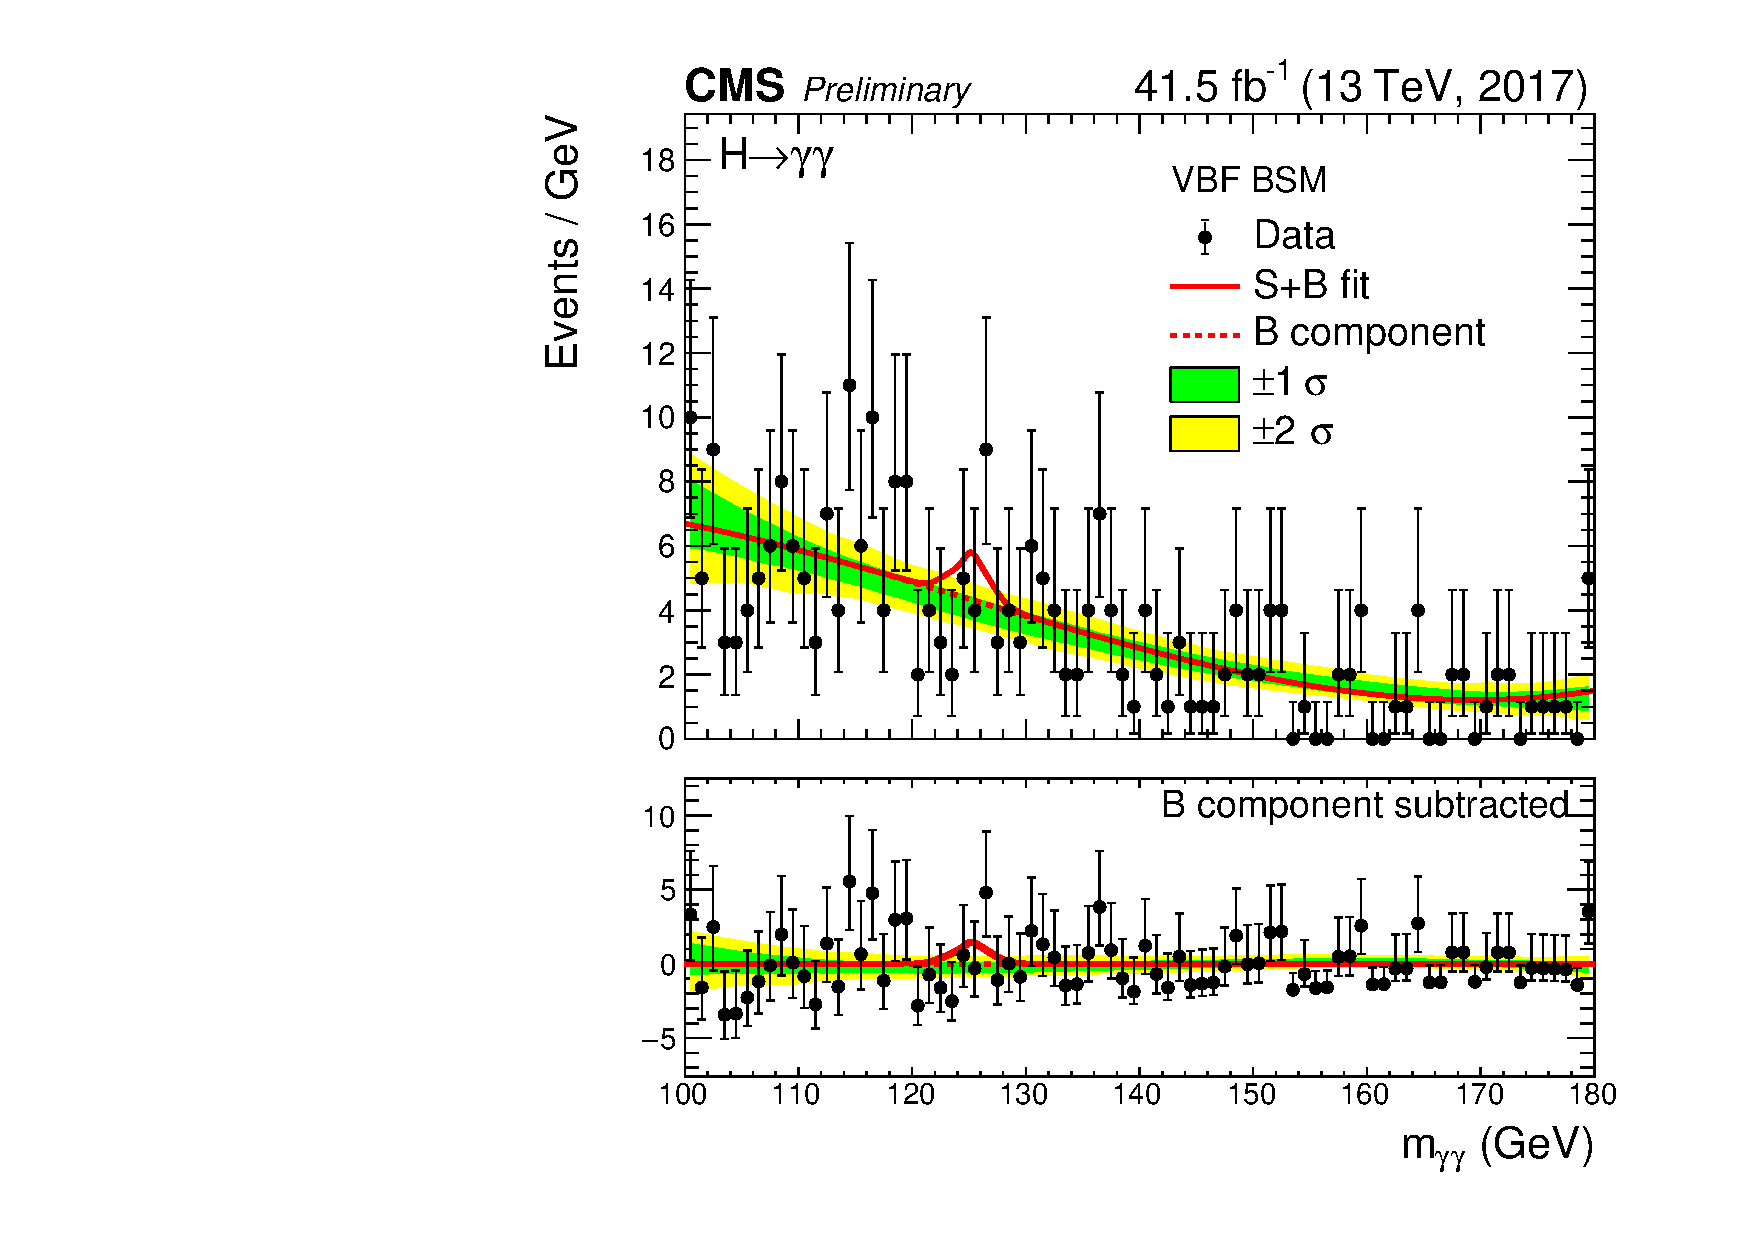
\includegraphics[width=0.49\textwidth]{Figures/Appendices/_forAppendix2017ch2_RECO_VBFTOPO_BSM_13TeV.pdf}
  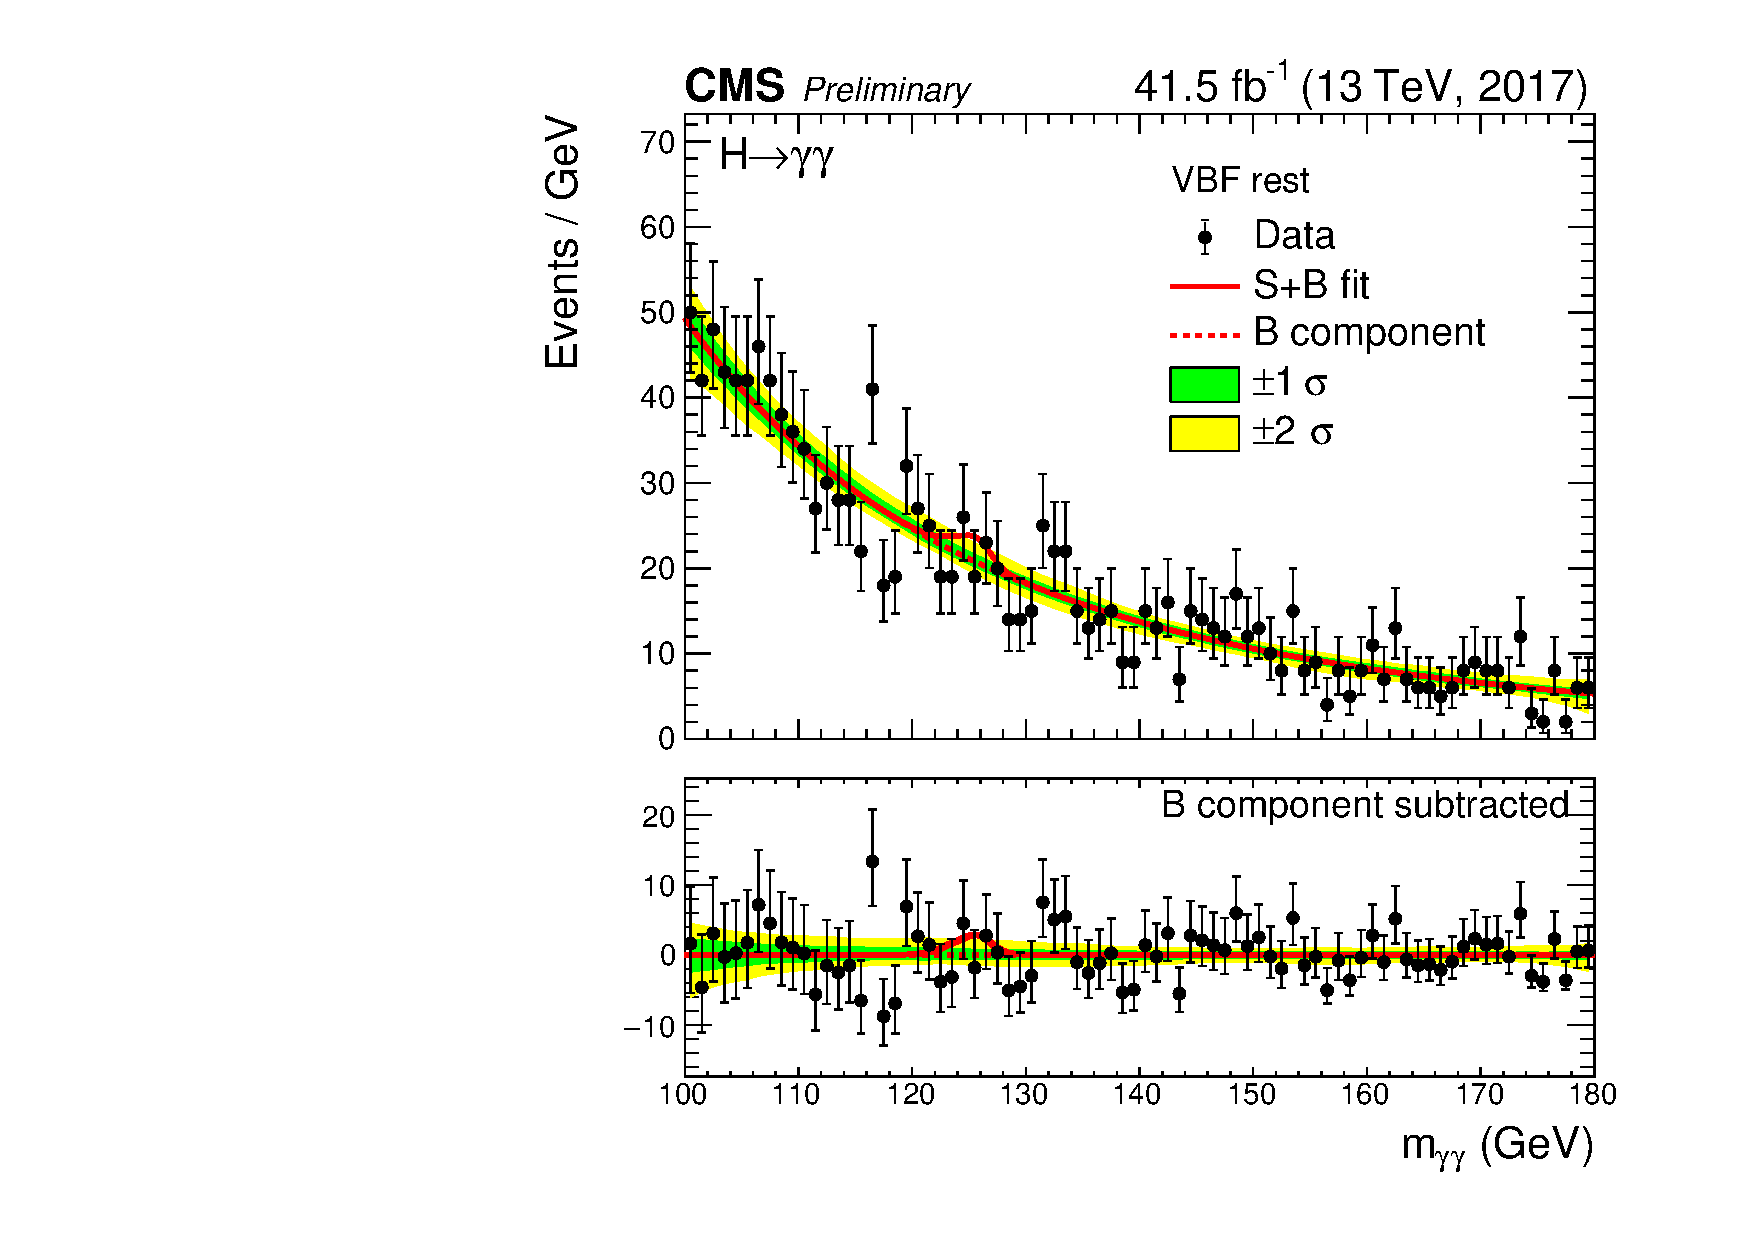
\includegraphics[width=0.49\textwidth]{Figures/Appendices/_forAppendix2017ch2_RECO_VBFTOPO_REST_13TeV.pdf}
  \caption[Signal plus background fits to data.]
  {
    Data points (black) and signal plus background model fit are shown. 
    The one standard deviation (green) and two standard deviation (yellow) bands 
    include the uncertainties in the background component of the fit. 
    The solid red line shows the contribution from the total signal, plus the background contribution. 
    The dashed red line shows the contribution from the background component of the fit. 
    The bottom plot shows the residuals after subtraction of this background component.
  }
\end{figure}
